\documentclass[11pt]{report}
%\usepackage{fullpage}
\usepackage{parskip}
\usepackage{titlesec}
\usepackage{xcolor}
\usepackage{subcaption}
\usepackage{algorithm}
\usepackage[noend]{algpseudocode}
\algnewcommand{\LineComment}[1]{\State \(\triangleright\) #1}
\makeatletter
\def\BState{\State\hskip-\ALG@thistlm}
\makeatother
\usepackage{comment}
\usepackage{inputenc}
\usepackage{csquotes}
\usepackage{float}
%\newfloat{algorithm}{t}{lop}
%\excludecomment{figure}
\usepackage[backend=biber,maxcitenames=1]{biblatex}
\bibliography{library}
\renewbibmacro{in:}{}
\usepackage[]{graphicx}
\graphicspath{{img/}}
\usepackage{lmodern}
\renewcommand{\baselinestretch}{1.02}
\usepackage{xargs}                      % Use more than one optional parameter in a new commands
\usepackage[]{xcolor}  % Coloured text etc.
\usepackage[colorinlistoftodos,prependcaption,textsize=tiny]{todonotes}
%\newcommand\todo[1]{\textcolor{red}{#1}}
\newcommandx{\unsure}[2][1=]{\todo[linecolor=red,backgroundcolor=red!25,bordercolor=red,#1]{#2}}
\usepackage{graphicx}
\usepackage[space]{grffile}
\usepackage{latexsym}
\usepackage{textcomp}
\usepackage{longtable}
\usepackage{multirow,booktabs}
\usepackage{amsfonts,amsmath,amssymb}
% You can conditionalize code for latexml or normal latex using this.
\newif\iflatexml\latexmlfalse
\usepackage[english]{babel}
\DeclareMathOperator*{\argmin}{arg\,min}
\DeclareMathOperator*{\argmax}{arg\,max}
\usepackage{sectsty}
\allsectionsfont{\normalfont\scshape}
\usepackage{fancyhdr}
\pagestyle{fancyplain}
\fancyhead{}											% No page header
\fancyfoot[L]{}											% Empty 
\fancyfoot[C]{}											% Empty
\fancyfoot[R]{\thepage}									% Pagenumbering
\renewcommand{\headrulewidth}{0pt}			% Remove header underlines
\renewcommand{\footrulewidth}{0pt}				% Remove footer underlines
\setlength{\headheight}{13.6pt}
\PassOptionsToPackage{hyphens}{url}
%\usepackage{hyperref}
\usepackage{url}
%\usepackage{hyperref}
%\def\UrlBreaks{\do\/\do-}

\title{Machine Learning-based Indoor Localization for Micro
  Aerial Vehicles}
\author{Volker Strobel}
\date{\today}

\begin{document}
\maketitle
\begin{abstract}
  Widespread applications, ranging from surveillance to search and
  rescue operations, make Micro Air Vehicles (MAVs) versatile
  platforms. However, MAVs have limited processing power due to their
  small size and cannot fall back on standard localization techniques
  in the indoor environment.
  %Therefore, the ubiquitous use of MAVs is
  %still impeded.
  To address this issue, an efficient on-board
  localization technique using machine learning was developed in the
  scope of this thesis.
  % The development, software and hardware implementation, and
  % results of the localization system are presented.

  The vision-based approach estimates $x,y$-coordinates within a known
  and modifiable indoor environment. Its computational power is
  scalable to different platforms, trading off speed and
  accuracy. Histograms of textons---small characteristic image
  patches---are used as features in a $k$-Nearest Neighbors ($k$-NN)
  algorithm. Several possible $x,y$-coordinates that are outputted by
  this regression technique are forwarded to a particle filter to
  neatly aggregate the estimates and solve positional ambiguities.
  % Promising results were obtained for all tasks: waypoint
  % navigation, accurate landing, and stable hovering in the indoor
  % environment.
  To predict the performance of the algorithm in different
  environments an evaluation technique is developed. It compares
  actual texton histogram similarities to ideal histogram similarities
  based on the distance between the underlying $x,y$-positions. The
  technique assigns a loss value to a given set of images, enabling
  comparisons between environments and the identification of critical
  positions within an environment. To compare maps before modifying an
  environment, a software tool was created that creates synthetic
  images that could be taken during an actual flight.

%The
%best one, the worst one and the one with median loss were printed out
%to compare their performance in the real-world. In fact, the results
%could be replicated on these maps.

%  We conducted several flight tests to evaluate the performance of the
%  approach. A comparison of the localization technique with the ground
%  truth showed an average error of 50\,cm. In a triggered landing
%  setting, the MAV correctly landed in specified areas, in ten out of
%  ten trials. The method was tested on 46 high-resolution images to
%  identify well-performing maps.

  We conducted several flight tests to evaluate the performance of the
  approach. A comparison of the localization technique with the ground
  truth showed promising results. In a triggered landing setting, the
  MAV correctly landed in specified areas. The map evaluation
  technique was applied to various high-resolution images to identify
  suitable maps.


%The development, software and hardware
%implementation, and results of the localization system are presented.
%The estimates of the proposed system are compared to the ground truth in five on-ground and two
%in-flight experiments with promising results.

  The presented approach is based on three pillars: (i) a shift of
  processing power to a pre-flight phase to pre-compute
  computationally complex steps, (ii) lightweight and adaptable
  algorithms to ensure real-time performance and portability to
  different platforms, (iii) modifiable environments that can be
  tailored to the presented algorithm. These pillars can build a
  foundation for efficient localization in various GPS-denied
  environments.
\end{abstract}
\tableofcontents
%\listoffigures
%\listoftables
\chapter{Introduction}
\label{chap:introduction}

In the world of automation, micro aerial vehicles (MAVs) provide
unprecedented perspectives for domestic and industrial
applications. They can serve as mobile surveillance cameras, flexible
transport platforms, or even as waiters in restaurants. However,
indoor employment of these vehicles is still hindered by the lack of
real-time position estimates. The focus of this thesis is, thus, the
development of efficient indoor localization for MAVs combining
computer vision and machine learning techniques.

%Many crimes over the last decades have been solved thanks to footage
%captured by surveillance cameras. However, stationary cameras can be
%easily manipulated or avoided once it is known where they are
%located. One possible solution may be the use of micro aerial vehicles
%(MAVs) for surveillance. To date, indoor employment of these vehicles
%is still hindered by several limitations. The focus of this thesis is,
%thus, the development of accurate and fast indoor localization for
%MAVs combining computer vision and machine learning techniques.

%Since precision and reliability are crucial for safe flight,
% autonomous indoor navigation of an MAV is a challenging task.
While unmanned aerial vehicles (UAVs) for outdoor usage can rely on
the global positioning system (GPS), this system is usually not
available in confined spaces and would not provide sufficiently
accurate estimates in cluttered environments. If sufficient
computational and physical power is available, a typical approach to
estimate a UAV's position is by using active laser
rangefinders~\cite{grzonka2009towards,bachrach2009autonomous}.
Although this approach is used in some simultaneous localization and
mapping (SLAM) frameworks, it is usually not feasible for MAVs because
they can carry only small payloads. A viable alternative are passive
computer vision techniques. Relying on visual information scales down
the physical payload since cameras are often significantly lighter
than laser
rangefinders~\cite{blosch2010vision,angeli20062d,ahrens2009vision}.
Additionally, many commercially available drones are already equipped
with cameras.  In contrast to other existing approaches, it does not
rely on additional information, such as data from the inertial
measurement unit (IMU). The only required tool is a camera, which
minimizes possible points of failure. Cameras are not only lightweight
but also robust to external influences like magnetic fields. This
minimizes points of failure.
\begin{figure}[h!]
\begin{center}
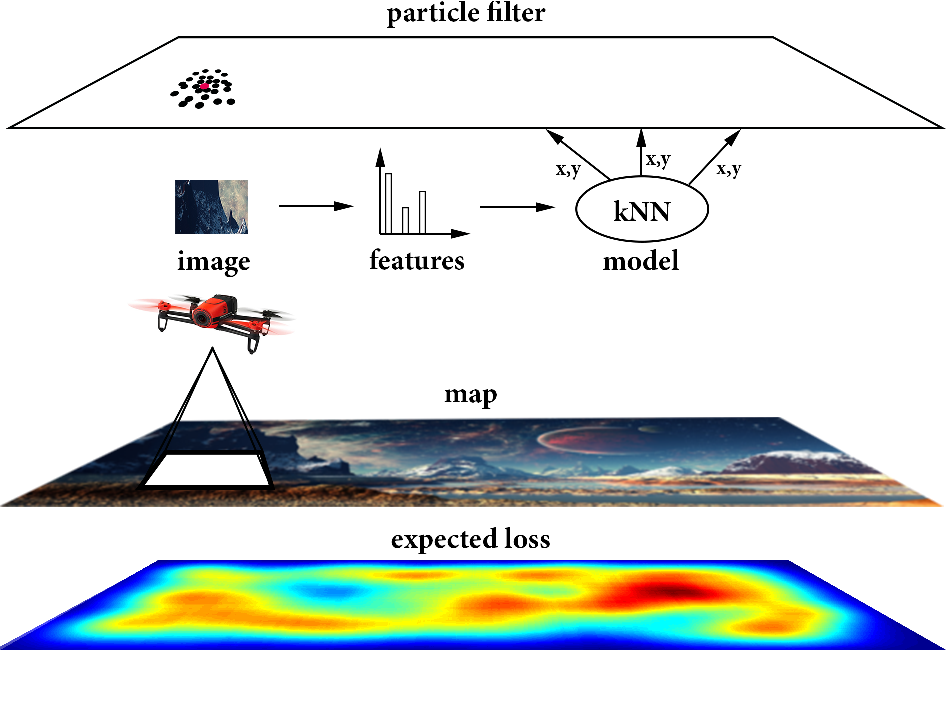
\includegraphics[width=0.75\columnwidth]{nutshell}
\caption{{\label{fig:highleveloverview} The figure illustrates the
    developed system from a high-level perspective. A feature
    vector---the texton histogram---is extracted from the current
    camera image of the UAV. The feature vector is forwarded to a
    machine learning model that uses a $k$-Nearest Neighbors algorithm
    to output $x,y$-position estimates. These estimates are passed to
    a particle filter, which filters position estimates over time and
    outputs a final position estimate (red point). The expected loss
    shows regions in the map where a lower localization accuracy is
    expected. The average expected loss can be used as ``fitness
    value'' of a given map.%
  }}
\end{center}
\end{figure}
However, this reduced physical payload is not without cost: it must be
traded off against the higher computational payload for the on-board
CPU. Vision-based position estimation is usually a time-consuming and
memory-intense procedure. One way to overcome this problem is to
process the data on a powerful external processor by establishing a
wireless connection between the MAV and a ground station. Such
off-board localization techniques often lack the versatility to
function in changing environments, though, due to factors---such as
the bandwidth, delay, or noise of the wireless
connection---interfering with the system's reliability.

The developed framework uses a computationally efficient machine
learning approach to estimate the position, which circumvents the
requirement to store a map in the UAV's `mind'. To assign
$x,y$-coordinates to images in a training set, keypoints in the
current image and a map image are detected in a pre-flight phase. This
is then followed by finding a homography---a perspective
transformation---between them to locate the current image in the
map. As an alternative images can be aligned with high-precision
position estimates from a motion tracking system.

%For example, a standard technique for 3D pose estimation extracts
%keypoints of the current camera image and a map image and then
%determines a homography between both keypoint sets. While this
%approach has been used for visual SLAM for
%MAVs~\cite{blosch2010vision}, the pipeline for accurate feature
%detection, description, matching, and pose estimation is
%CPU-intensive~\cite{kendall2015posenet}.

In the next step, the complexity of these images is reduced by
determining their histogram of textons---small characteristic image
patches~\cite{varma2005statistical}. New images can then also be
encoded by texton histograms and matched to images with known
$x,y$-positions using the $k$-Nearest Neighbors ($k$-NN)
algorithm. The $k$-NN estimates are passed to a particle filter to
neatly aggregate the estimates and solve positional ambiguities. The
computational effort of the approach can be adjusted by modifying the
amount of extracted patches and used particles, resulting in a
trade-off between accuracy and execution
frequency. Figure~\ref{fig:highleveloverview} summarizes the
algorithm.

In the presented approach, computational power will be shifted to an
offline training phase to achieve high-speed during live operation. In
contrast to visual SLAM frameworks, this project considers scenarios
in which the environment is known beforehand or can be even actively
modified. The environment is non-dynamic and planar, therefore, the
UAV will make use of texture on the bottom or ceiling of the
environment. This opens the door for improving the accuracy of the
algorithm by changing the map. On the basis of desired characteristics
of a given map, an evaluation technique was developed that determines
the suitability of an environment for the presented approach. This technique
allows for spotting distant regions with similar image features, which
could lead to deteriorated performance. The evaluation can be
performed using a given map image or recorded images during flight. In
the former case, synthetic images will be generated from the map image
that simulate images taken during flight.


\section{Problem Statement and Research Questions}
\label{sec:researchquestions}

The goal of this thesis is to develop a fast localization technique
for MAVs. Therefore, we formulated the following problem statement:

\par
\begingroup
\leftskip=0.7cm % Parameter anpassen
\noindent \textbf{Problem statement:} \emph{How can
    $x,y$-coordinates be estimated in real-time and on-board of an
    MAV?} %ab hier der Text, der eingerückt werden soll
\par
\endgroup

It is assumed that the UAV flies at an approximately constant height,
such that the estimation of height is not necessary. Since it is
intended to further reduce the size of MAVs, lightweight and scalable
position estimation algorithms are needed. The problem was addressed
by combining computer vision and machine learning techniques for
achieving real-time position estimates. We focus on the following
research questions (RQs):
\begin{itemize}
\item \textbf{RQ\,1:} ``\emph{Can 2D positions be estimated in real-time using a
    machine learning approach on a limited processor in a modifiable
    indoor environment?}''\vspace*{0.05cm}\\
  Real-time position estimates can pave the way for autonomous flight
  of MAVs in various indoor environments; pursuing an ``on-board
  design'' to make the MAV independent of an external ground station
  is an important step for security and versatility.
%\item Is accurate real-world localization regression possible when the
%  training data comprises synthetic data only?
\item \textbf{RQ\,2:} \emph{``How can we predict and evaluate the suitability of a
    given map for the developed localization approach?''}  \vspace*{0.15cm}\\
  Computer vision techniques are commonly limited to environments with
  sufficient and informative texture. If an environment can be
  evaluated before actually flying in it, the performance of the
  approach can be predicted and possible dangers prevented.
\end{itemize}

\section{Contributions}
\label{sec:contributions}

The first contribution of this thesis is a machine learning-based
indoor localization system that runs in real-time on board of an MAV,
paving the way to an autonomous system. In contrast to existing
\emph{active} approaches, the developed \emph{passive} approach only
uses a monocular downward-looking camera. Since computer vision-based
localization approaches yield noisy estimates, a variant of a particle
filter was developed that aggregates estimates over time to produce
more accurate predictions. It handles the estimates of the $k$-NN
algorithm in an integrative way and resolves position ambiguities. The
method is a global localization system and does not suffer from error
accumulation over time.

The second contribution is a map evaluation technique that predicts
the suitability of a given environment for the presented algorithm. To
this end, a synthetic data generation tool was developed that creates
random variations of an image. The tool simulates different viewing
angles, motion blur, and lighting settings; the generated synthetic
images are labeled with $x,y$-coordinates based on the 3D position of
the simulated camera model.

The developed software is made publicly available. It encompasses (i)
the localization algorithm as part of the Paparazzi autopilot
system~\cite{brisset2006paparazzi}, which consists of the texton-based
approach in combination with a particle filter (ii) software for
augmenting an image with synthetic views, (iii) a script for
evaluating a map based on histograms and corresponding
$x,y$-positions.


\section{Thesis Outline}
\label{sec:outline}

The remainder of this thesis is structured as follows.
Chapter~\ref{chap:relatedwork} surveys existing indoor localization
approaches related to this thesis. In Chapter~\ref{chap:methods}, the
developed texton-based approach is presented and its components, the
$k$-NN algorithm and the particle filter, are introduced. Details about
the synthetic data generation tool and map evaluation technique are
also given. Chapter~4 describes the setup and
results of the on-ground and in-flight experiments. The results are
then discussed in Chapter~5. Finally, we draw our
conclusions and indicate future research directions in
Chapter~6.%\ref{chap:conclusion}.

\chapter{Related Work}
\label{chap:relatedwork}

This chapter discusses advantages and disadvantages of different
approaches for indoor localization.
%and contrast them to the proposed
%method.
While a wide range of methods for indoor localization exists, from
laser range scanners over depth cameras to radio-frequency
identification tag (RFID) based localization, we only discuss methods
that use the same technical and conceptual setup---localization with a
monocular camera.

One distinguishes two types of robot localization: local techniques
and global techniques~\cite{fox1999monte}. Local techniques need an
initial reference point and estimate coordinates based on the change
in position over time. Once they lost track, the position can
typically not be recovered. The approaches also suffer from ``drift''
since errors are accumulating over time. Global techniques are more
powerful and do not need an initial reference point. They can recover
when temporarily losing track and address the \emph{kidnapped robot
  problem}, in which a robot is carried to an arbitrary
location~\cite{engelson1992error}.

Target systems and test environments are often too different to draw
comparisons: factors, such as the size of the environment, the speed
of the robot or camera, or the processor play crucial roles for the
evaluation. Therefore, comparing the accuracy and run-time of
different localization methods is difficult.

% The annual Microsoft Indoor Localization Competition aims at setting
% a standardized testbed for comparing near real-time indoor
% localization technologies~\cite{microsoft}. However, since the
% competition does not require lightweight platforms and allows the
% use of external infrastructure such as WiFi routers, no vision-only
% approach has yet been presented at the competition.

\section{Vision-based Localization Methods}

\subsection{Fiducial Markers}
\label{sec:fiducialmarkers}

Fiducial markers (Figure~\ref{fig:aruco}), which are often employed in
augmented reality
applications~\cite{kato1999marker,garrido2014automatic}, have been
used for UAV localization and
landing~\cite{eberli2011vision,bebop2015}. The markers encode
information in the spatial arrangement of black-and.white or colored
image patches. Their corners can be used for estimating the camera
pose at a high frequency. The positions of the markers in an image are
usually determined with \emph{local thresholding}. Local thresholding
is a simple method for separating objects---salient image
regions---from a background. Its output is a binary image with two
states: foreground (markers) and background. Marker positions are then
often further refined by removing improbable shapes, yielding an
adjusted version of possible marker positions~\cite{aruco2014}.

An advantage of fiducial markers is their widespread use, leading to
technically mature open-source libraries, including
ArUco~\cite{aruco2014} and ARToolKit~\cite{kato1999marker}. Given
adequate lighting conditions, markers can be used in a wide variety of
environments~\cite{hornecker2005using}. This makes them suitable for
indoor localization. A drawback of the approach is that motion blur,
which frequently occurs during flight, can hinder the detection of
markers~\cite{albasiouny2015mean}. Furthermore, partial occlusion of
the markers through objects or shadows break the detection; each
marker needs to be fully in the camera
view~\cite{hornecker2005using}. Another downside is that markers might
be considered as visually unpleasant and may not fit into a product or
environmental design~\cite{chu2013halftone}. They offer little
flexibility, since one has to rely on predefined marker
dictionaries. Additionally, marker-based approaches always require the
modification of the environment. Like most vision-based approaches,
the detection of markers is prone to changes in lighting conditions
and may not work in low-contrast settings~\cite{hornecker2005using}.

%There is no direct way to modify the time complexity of the algorithm.

% TODO: which errors have been achieved

\begin{figure}[h!]
\begin{center}
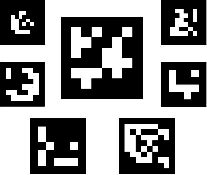
\includegraphics[width=0.3\columnwidth]{markers}
\caption{{\label{fig:aruco}
Examples of fiducial markers of the ArUco library.%
}}
\end{center}
\end{figure}

\subsection{Homography Determination \& Keypoint Matching}
\label{sec:keypointmatching}

A standard approach for estimating camera pose is detecting and
describing keypoints of the current view and a reference
image~\cite{se2002global}, using algorithms such as Scale-invariant
feature transform (\textsc{Sift})~\cite{lowe1999object}, followed by
finding a homography---a perspective transformation---between both
keypoint sets (Figure~\ref{fig:sift}). A keypoint is a salient image
location described by a feature vector. Depending on the algorithm, it
is invariant to different viewing angles and scaling.

The \textsc{Sift} algorithm transforms an image into a set of image
features. It works in four subsequent stages using gray-scale images
as input:
\begin{enumerate}
\item \emph{Maxima detection:} The image is convolved with the
  \emph{Difference of Gaussian} blob detector. By varying the variance
  of the Gaussian distribution, the maxima---potential
  keypoints---across different scales and spaces can be detected.
\item \emph{Refinement of keypoints:} The potential keypoints are
  refined by removing maxima with small contrast and non-discriminative
  edges.
\item \emph{Orientation assignment:} A histogram of the gradient
  orientations around the keypoint is created. The most frequent value
  indicates a the keypoint orientation.
\item \emph{Keypoint description:} The local image gradients are
  transformed into a feature vector by describing pixels around a
  radius of a keypoint.
\end{enumerate}

To locate the current view in the reference image, keypoints from one
set are matched with their nearest neighbor in the other set using the
Euclidean distance between their feature vectors. Based on the matched
keypoint descriptions, a homography is calculated between the
coordinates of both keypoint sets. This allow for locating the current
view in the reference image. The calculation of the homography matrix
($H$) needs four matches between both keypoint sets. Usually many more
points are available, leading to an overdetermined equation. The
solution to $H$ is then computed by minimizing the errors of between
all the projected keypoints in a least-square sense.

While this \emph{homography-based} approach is employed in frameworks
for visual Simultaneous Localization and Mapping (SLAM), the pipeline
of feature detection, description, matching, and pose estimation is
computationally complex~\cite{kendall2015posenet}. Therefore, ground
stations for off-board processing or larger processors are usually
needed for flight control. In this thesis, the homography-based
approach is used in a pre-flight phase to assign $x,y$-coordinates to
images.
\begin{figure}[h]
\begin{center}
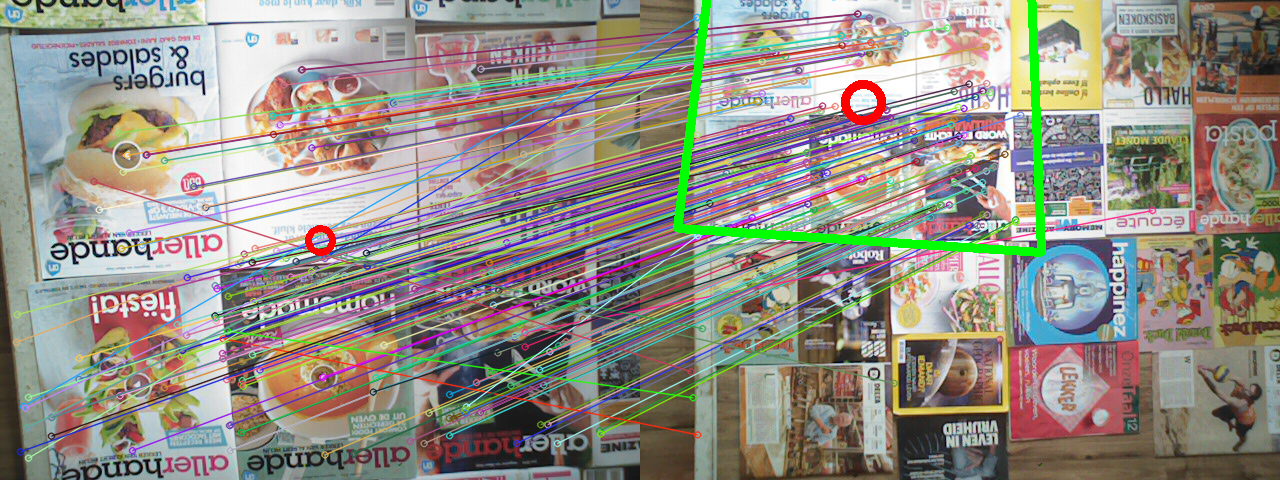
\includegraphics[width=0.85\columnwidth]{sift}
\caption{{\label{fig:sift}Perspective transformation between keypoints of the current
    image (left) and the reference or map image (right).%
  }}
\end{center}
\end{figure}
The approach has been employed for global localization for UAVs:
\citeauthor{blosch2010vision}~\cite{blosch2010vision} evaluate it on a
$3.5\,m \times 2\,m$ area and achieve a root mean square (RMS)
positional error below $10\,cm$ in $x,y,z$-direction. Calculations are
executed on a powerful ground station, which is connected to the UAV
with a USB cable. Subsequent research has brought the algorithm on
board of UAVs~\cite{achtelik2011onboard}, achieving a frequency of
10\,Hz with a 1.6 GHz on-board processor with 1 GB RAM. However, the
required processing power is still too complex for small
MAVs. %~\cite{de2009design}.

\subsection{Convolutional Neural Networks}

Convolutional neural networks (CNNs) are a specialized machine
learning method for image processing~\cite{lecun1998gradient}. The
supervised method has outperformed other approaches in many computer
vision challenges~\cite{dosovitskiy2014discriminative}. CNNs consist
of multiple neuron layers, which represent increasing levels of
abstraction~\cite{lecun1998gradient}. While their training is usually
time-consuming, predictions with CNNs often takes only few
milliseconds, shifting computational effort from the test phase to the
training phase. CNNs have been used as a robust alternative for
keypoint detection and description if images were
perturbed~\cite{dosovitskiy2014discriminative} but needed more
computation time than \textsc{Sift}.

In recent work, \citeauthor{kendall2015posenet} present a framework
for regressing camera positions based on
CNNs~\cite{kendall2015posenet}. The method achieves an accuracy of
approximately 50\,cm in indoor environments with a spatial extent
between $2 \times 0.5 \times 1\,m^3$ and $4 \times 3 \times
1.5\,m^3$. The approach is rather robust to different lighting
settings, motion blur, and varying camera intrinsics. The approach
predicts positions on a modern desktop computer in short
time. However, in our implementation---employing the scientific
computing framework Torch~\cite{collobert2011torch7}---the approach
was still computationally too involved for achieving real-time
prediction on an Odroid XU-4 single board computer.

\subsection{Optical Flow}
\label{sec:opticalflow}

Optical flow algorithms are biologically inspired methods for
navigation---taking inspiration from insects and
birds~\cite{ruffier2003bio}. They estimate the apparent motion between
successive images, for example, by comparing the positions of their
keypoints~\cite{chao2013survey}.
% and more specific methods have been put forth\todo{for example}.
Optical flow methods belong to the class of \emph{local} localization
techniques and can only estimate the position relative to an initial
reference point. The approaches suffer from accumulating errors over
time and typically do not provide a means for correcting these errors.

\citeauthor{chao2013survey}~\cite{chao2013survey} compare advantages
and disadvantages of different optical flow algorithms for the use
with UAV navigation. Most approaches are computationally rather
complex~\cite{mcguire2016local}. To render on-board odometry feasible
for small MAVs, \citeauthor{mcguire2016local}~\cite{mcguire2016local}
introduce a lightweight optical flow variant. The algorithm uses
compressed representations of images in the form of edge histogram to
calculate the flow.

\section{Texton-based Methods}
\label{sec:textonbasedapproaches}

Textons are small characteristic image patches; their frequency in an
image can be used as image feature
vector. \citeauthor{varma2005statistical}~\cite{varma2005statistical}
originally introduced textons for classifying different textures,
showing that they outperform computationally more complex algorithms,
like Gabor filters~\cite{varma2005statistical}. For the
classification, the approach compares texton histograms between a
training set and the test sample and the class of the closest training
sample is assigned to the test
sample. %leading to similar texton histograms
                           %compared to the histograms when full
                           %sampling is used.
A texton histogram is obtained by extracting patches from an image and
comparing them to all textons in a ``texton dictionary''. The
frequency of the most similar texton is then incremented in the
histogram.

Texton histograms are flexible image features and their extraction
requires little processing time, which makes them suitable for MAV
on-board algorithms. The approach allows for adjusting the
computational effort by modifying the amount of extracted image
patches, resulting in a trade-off between accuracy and execution
frequency.  A disadvantage is that it discards all information about the spatial
arrangement of texton, %---it does not make use of the
%\emph{Where} of the information, just of the \emph{What},
so that different images can have the same histogram.
%Additionally, it performs better than or, at least, equal to
%optical flow estimations.

\citeauthor{de2009design}~\cite{de2009design} use textons
as image features to distinguish between three height classes of the
MAV during flight. Using a nearest neighbor classifier, their approach
achieves a height classification accuracy of approximately 78\,\% on a
hold-out test set. This enables a flapping-wing MAV to roughly hold
its height during an experiment. In another work,
\citeauthor{de2012appearance}~\cite{de2012appearance} introduce the
\emph{appearance variation cue}, which is based on textons, for
estimating the proximity to objects~\cite{de2012appearance}.
% Since closer objects should have less variation, these objects
% should appear less varied.
Using this method, the MAV achieves a high accuracy for collision
detection and can avoid obstacles in a $5m \times 5m$ office space.

In the scope of this thesis, an efficient \emph{global} localization
was developed that draws upon the lightweight character of
texton-based approaches and combines their flexibility with the
advantages of homography-based approaches.

\chapter{Methods}
\label{chap:methods}

This section describes the ideas behind the developed approach, the
hardware, and software implementations.
% An overview of the entire process is sketched out in
% Figure~\ref{fig:overview}.
The approach is based on three ``pillars'': (i) a shift of processing
power to a pre-flight phase to pre-compute computationally complex
steps, (ii) lightweight and adaptable algorithms to ensure real-time
performance and portability to different platforms, (iii) modifiable
environments to get the most out of the approach. The pseudo code in
Algorithm~\ref{alg:trexton_run} shows a high-level overview of the
parts of the framework. Details about the parts of the framework and
the pillars will be given in separate sections.
% All developed software is made publicly available, the corresponding
% links are given in the respective sections.
\begin{algorithm}
    \caption{High-level texton framework}
    \label{alg:trexton_run}
    \begin{algorithmic}[1]
      \State $t \gets 0$
      % \State textons $\gets$ \Call{csv\_read\_textons}{}
      % \State ann $\gets$ \Call{load\_neural\_network}{}
      \State $\mathcal{X}_0 \gets$ \Call{init\_particles}{}
      \While {true}
      %\Procedure{Run\_Texton\_Framework}{}
      \State $t \gets t+1$ \State
      $I_t \gets$ \Call{Receive\_Img\_from\_Camera}{} \State
%      $\widetilde{I_t} \gets$ \Call{Standardize\_Image}{$I_t$} \State
      $\mathcal{H}_t \gets$ \Call{Get\_Texton\_Histogram}{$I_t$}
      \State $\mathbf{z}_t \gets$
      \Call{$k$-NN}{$\mathcal{H}_t$}
      %\State $f_t^x, f_t^y \gets$ \Call{Calc\_Flow}{$I_t$}
      \State $\mathcal{X}_t \gets$
      \Call{Particle\_Filter}{$\mathcal{X}_{t-1}, \mathbf{z}_t$}
      \State $x_t, y_t \gets$ \Call{Maximum\_a\_Posteriori\_Estimate}{$\mathcal{X}_t$}
%      \EndProcedure
      \EndWhile
\State \textbf{end}
    \end{algorithmic}
  \end{algorithm}  
  % \Call{Send\_Pos}{$x_t, y_t$}
\section{Hardware and Software}
\label{sec:hardware}

In our first approach, the commercially available Parrot AR.Drone2.0
was equipped with an Odroid XU-4 single board computer, a Logitech 525
HD webcam, and WiFi module. Figure~\ref{fig:comparison} shows the
setup. Instead of employing the AR.Drone2.0 processor, the camera
images were processed on the more powerful Odroid processor and the
resulting $x,y$-estimates were sent over a USB data link to the MAV
flight controller. The Odroid processor has a full operating system
(Ubuntu 15.04) and can run arbitrary Linux software.  However, the
additional weight through the modifications of the system resulted in
unstable flight performance. Therefore, we modified the system to
execute the localization algorithm directly on-board of the MAV and not
on the additional Odroid processor. To this end, the software had to
be ported from the high-level language Python to the low-level
language C without relying on many existing software libraries.
However, this step removed the need for the additional payload and
made the flight performance very stable. Also, it circumvented the
effort of buying and attaching an external processor, which can be
another point of failure. Another advantage is that the framework can
be easily ported to any UAV supported by the Paparazzi software. The
major disadvantage is that the on-board processors of many MAVs have a
lower performance than the Odroid processor.

\begin{figure}[h!]
\begin{center}
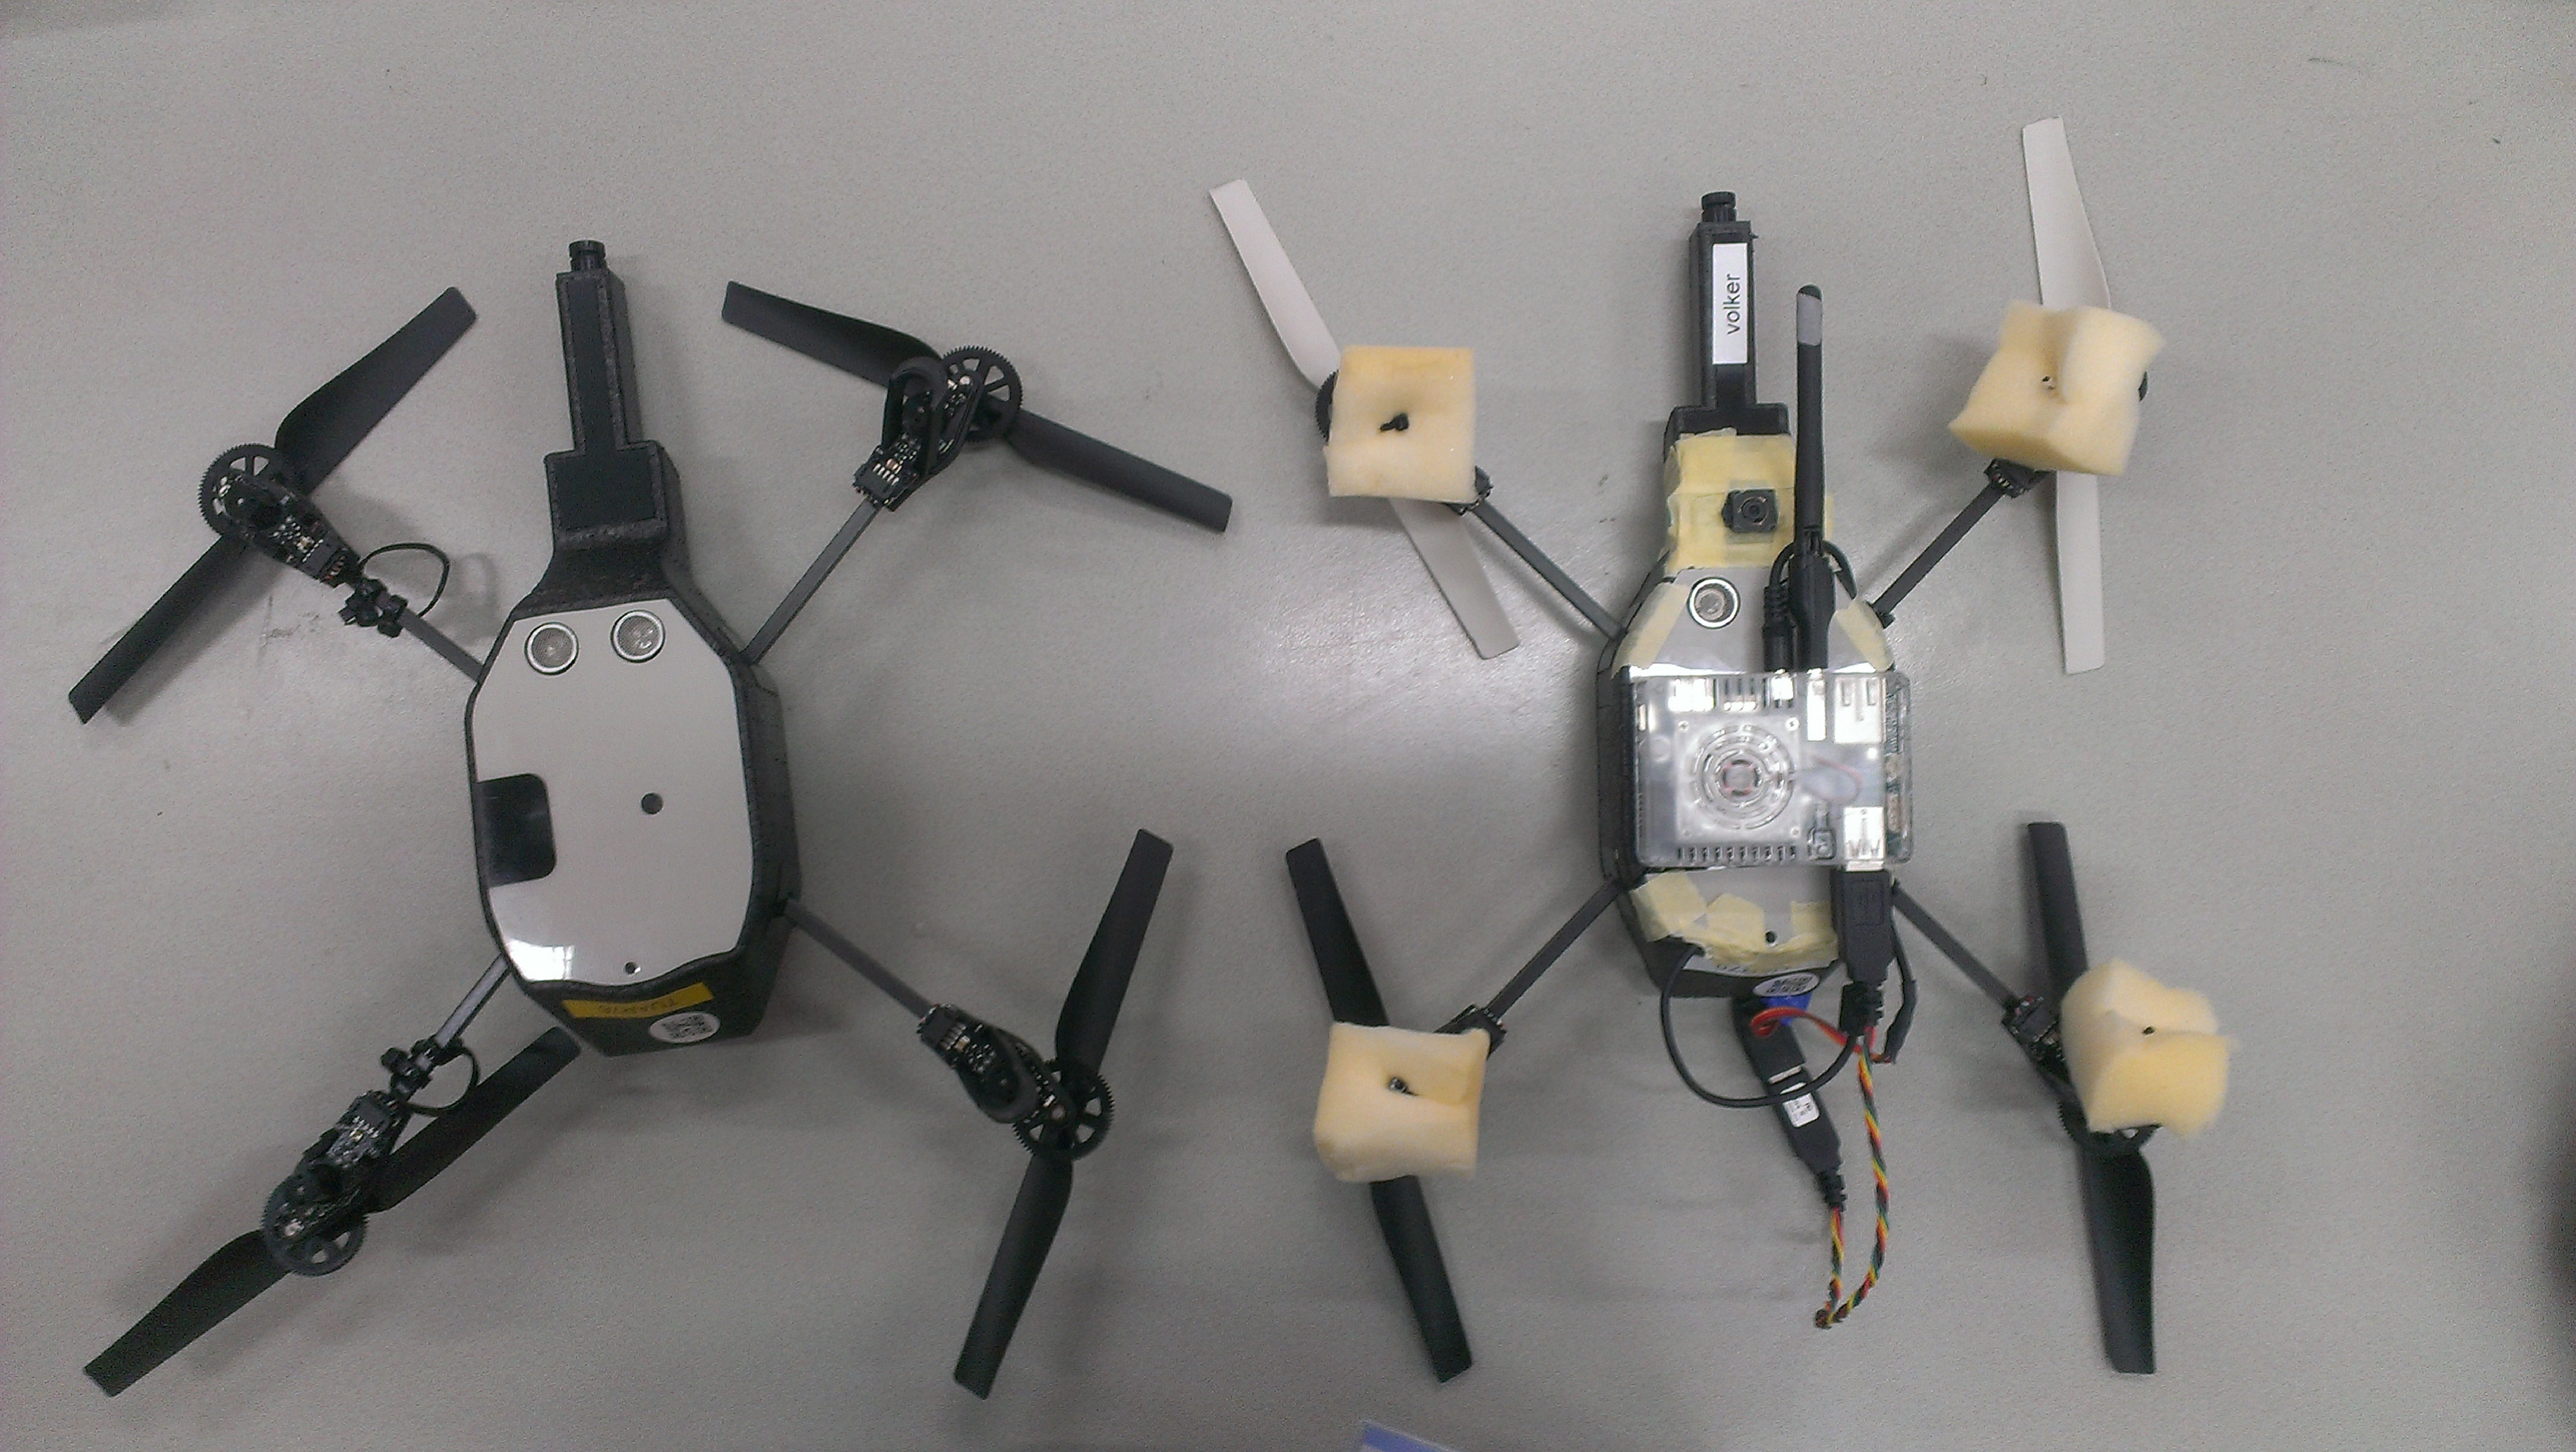
\includegraphics[width=0.7\columnwidth]{comparison}
\caption{{\label{fig:comparison}
Comparison of an unmodified Parrot AR.Drone.2.0 (left) and a
    modified version (right). The modified one was equipped with an
    Odroid XU-4 single board computer, a Logitech C525 HD camera, a
    WiFi module, and a USB connection between the Odroid board and the
    AR.Drone.2.0 flight controller.%
}}
\end{center}
\end{figure}

We decided to conduct all our tests with a quadcopter. Quadcopters
allow for navigating in arbitrary directions without changing their
yaw angle, show stable flight behavior, and often have high-resolution
cameras. We used the \emph{Parrot Bebop Drone} as a prototype. It is
equipped with a lithium-ion polymer battery that lasts for
approximately 11 minutes flying time. The UAV's dimensions are
$28 \times 32 \times 3.6$\,cm and it weighs 400\,g. It has two
cameras: a front camera and a downward-looking bottom camera. The
developed approach makes use of the bottom camera only. This camera
has a resolution of $640 \times 480$ pixels with a frequency of 30
frames per second. The UAV's processor is a Parrot P7 dual-core CPU
Cortex A9 with a tact rate of 800\,Mhz. It is equipped with 8~GB of
flash memory and runs a Linux operating system. The full
specifications of the UAV can be found on its official
website~\cite{bebop}.

The original Bebop software development kit was replaced with the
open-source autopilot software
Paparazzi~\cite{brisset2006paparazzi}. Paparazzi is used and advanced
at the Micro Aerial Vehicle Laboratory at the TU Delft. The software
provides a link between a ground station computer and the UAV to send
commands and receive telemetry data. Furthermore, it provides functions
for creating flight plans, plotting and logging telemetry data, and
uploading firmware to the UAV. Its modular approach allows for
combining functions regarding stabilization, localization, and control
of UAVs, which are executed on board of the MAV. Paparazzi supports a
wide range of commercially available aircrafts and associated
hardware.
%While the goal of the presented system is to
%rely solely on onboard processing, monitoring the system during
%evaluation on a ground station is important.
Figure~\ref{fig:gcs} shows the ground control station of Paparazzi.
%For collecting
%data, real-time visualization of the position estimates and enabling
%future users to keep track of the system states, a graphical user
%interface (GUI) with the Qt GUI Application development framework was
%developed in the scope of this thesis. The GUI is displayed in
%Figure~\ref{fig:gui}.
\begin{figure}[t]
\begin{center}
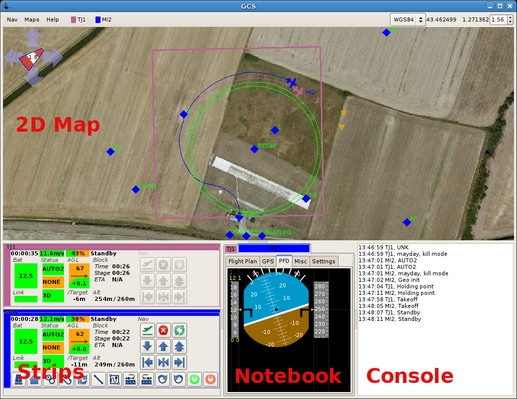
\includegraphics[width=0.7\columnwidth]{Gcs}
\caption{{\label{fig:gcs} The ground control station of the Paparazzi
    software. It displays information about the status of the UAV and
    provides functions for controlling the vehicle (from PaparazziUAV
    wiki \cite{paparazzi}).%
  }}
\end{center}
\end{figure}
%The GUI shows the position estimate of the developed framework, the
%ground truth position based on OptiTrack, the texton histogram, the
%Euclidean distances between OptiTrack and the system, the uncertainty
%of the system, and the correlation between the uncertainty and the
%Euclidean distance between the Optitrack and treXton estimates. The
%GUI can be accessed using the \emph{Tool} menu in Paparazzi.
%\begin{figure}[t]
%\begin{center}
%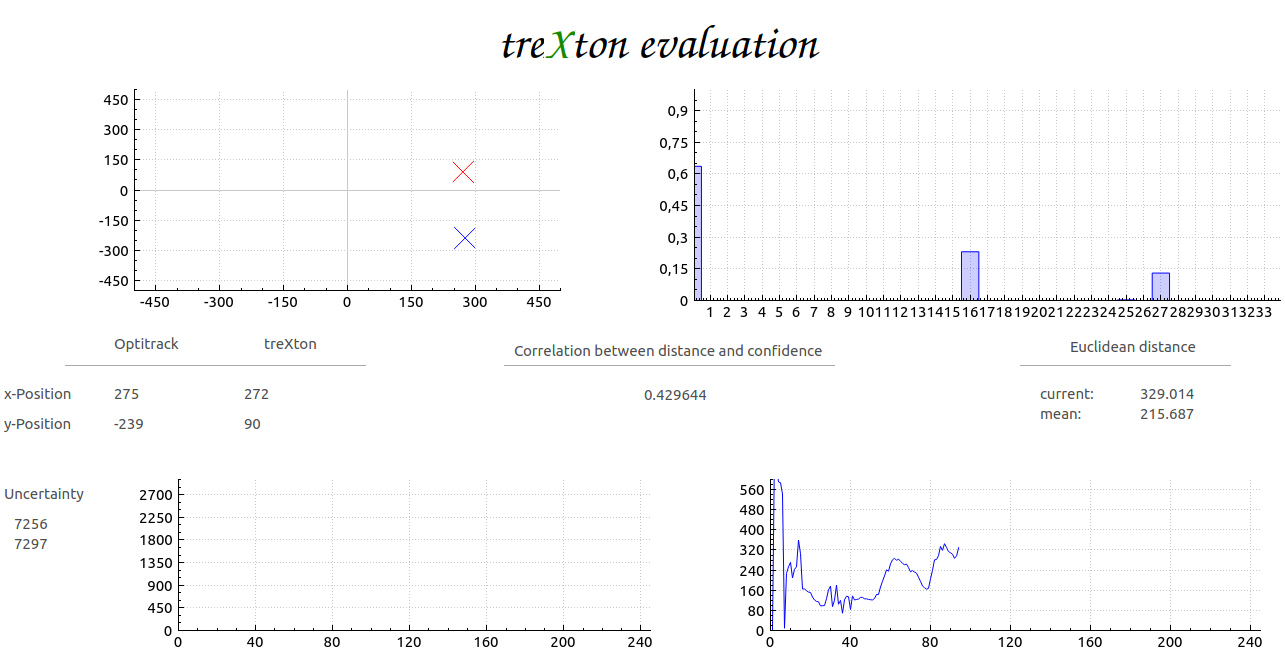
\includegraphics[width=\textwidth]{gui-cut}
%\caption{{\label{fig:gui} Screenshot of the GUI. From left to right
%    and top to bottom, it displays the position estimate of the
%    developed framework, the ground truth position based on OptiTrack,
%    the texton histogram, the Euclidean distances between OptiTrack
%    and the system, and the uncertainty of the system (based on the
%    spread of particles).%%
%  }}
%\end{center}
%\end{figure}
%

The presented approach is implemented as a module in Paparazzi's
computer vision framework. Since low-level routines like accessing
camera information or attitude control for different platforms are
already implemented in Paparazzi, the module can be readily used
across different platforms. Modules are written in the C programming
language and are cross-compiled on the host PC to make them suitable
for the UAV's processor. Afterwards, they are uploaded to the
microprocessor of the UAV to run them \emph{on board}. A downlink
connection---from the UAV to the ground station---permits monitoring
the state of the aircraft, for example information about speed,
altitude, position, or battery status.

\section{Preliminary Dataset Generation}
\label{sec:mapping}

% To exploit the advantages, and straighten out the disadvantages, we
% used the approach in a preprocessing step to obtain labeled training
% data of a known environment.  This allows to shift computational
% effort from the flight phase to a pre-flight phase---paving the way
% for autonomous flights of MAVs with limited processing power.

A main idea of the presented method is to shift computational effort
to a pre-flight phase. Since the MAV will be used in a fixed
environment, the results of these pre-calculations can be employed
during the actual flight phase. Supervised machine learning methods
need a training set to find a mapping from features to target
values. In this first step, the goal is to label images with the
physical $x,y$-position of the UAV at the time of taking the
image. Therefore, a method for obtaining the physical position of the
UAV is needed and GPS information is not available in the indoor
environment. In the presented approach, the image is later converted
to a texton histogram as described in the next section
(Section~\ref{sec:textons}).

One possible way to create the data set is to align the images with
high-precision position estimates from a motion tracking system.  The
camera forwards $640 \times 480$ pixel images in Y'UV422 color
space---a three-channel color space that encodes gray-scale
information in the channel Y and color information in the channels U
and V.
% Even low quality images can be mapped to the corresponding
% $x,y$-position.
The $x,y$-position is broadcast to the UAV via the ground station,
which is connected to the motion tracking system.  The data set is
created by saving the image with the corresponding position from the
motion tracking system on the MAV's hard disk. The approach yields
high-quality training sets since motion tracking systems can track
rigid bodies at a high frequency within an error of few
millimeters. Major disadvantages of the approach are that motion
tracking systems are usually expensive and time-consuming to move to
different environments. The workflow is illustrated in
Figure~\ref{fig:overviewn}.
\begin{figure}[h]
\begin{center}
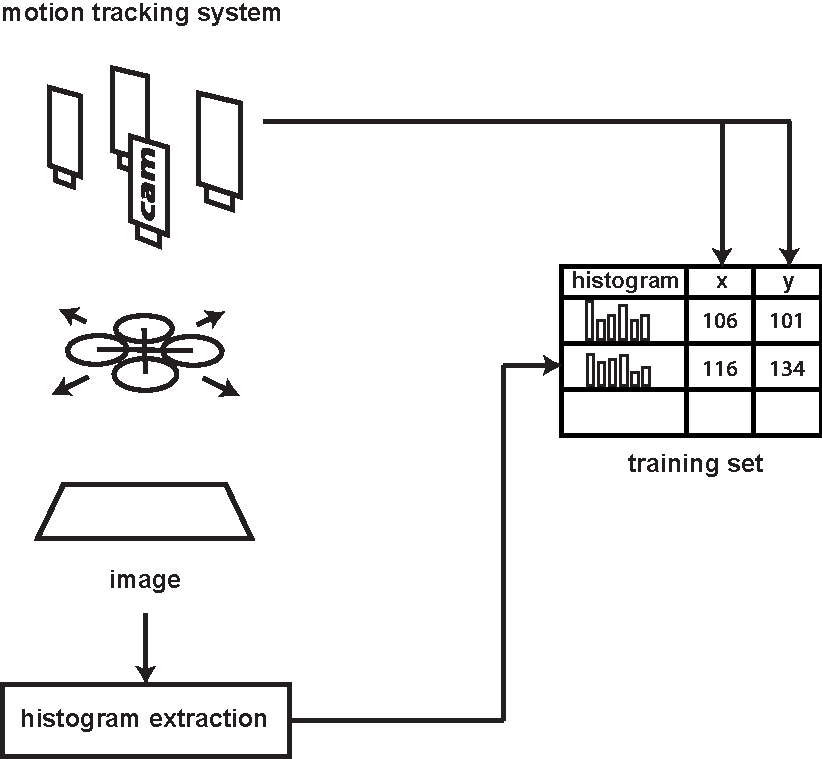
\includegraphics[width=0.56\columnwidth]{overview_new}
\caption{{\label{fig:overviewn}Training dataset generation if the motion tracking system is
    used. The texton histograms of the camera images during flight are
    extracted and aligned with the highly accurate position estimates
    of the motion tracking system. The result is a high-quality
    training set of texton histograms and corresponding
    $x,y$-positions.%
  }}
\end{center}
\end{figure}

As an alternative, we sought a low-budget and more flexible
solution. Of the presented approaches in Chapter~\ref{chap:relatedwork},
the homography-based approach (Section~\ref{sec:keypointmatching})
promises the highest flexibility with a good accuracy but also
requires the most processing time. Since fast processing time is not
relevant during the pre-flight phase, the approach is well-suited for
the problem.
% high matching quality for non-blurry images, it suffers from lacking
% robustness to noise and the high processing time requirements.  It
% is based on two associated cornerstones that are performed in an
% offline phase: the creation of a two-dimensional map and finding
% homographies homography.
The required image dataset can be obtained by using images gathered
during manual flight or by recording images with a hand-held
camera. To get a hyperspatial image of the scene for creating a map,
the images from the dataset have to be stitched together. The stitched
image has a higher resolution than the single images and contains a
greater range of detail (Figure~\ref{fig:orthomap}).  With certain
software packages the images can be ``orthorectified''by estimating
the most probable viewing angle based on the set of all
images. However, since a downward-looking camera is attached to the
UAV, most images will already be roughly aligned with the z-axis,
given slow flight~\cite{blosch2010vision}.  We used the freeware
software Microsoft Image Composite Editor (ICE)~\cite{ice} for the
stitching process. However, this closed-source software does not
publish details about its used techniques. As an open-source
alternative, the panorama photo stitching software
\emph{hugin}~\cite{hugin} is available. In our tests, Microsoft ICE
yielded better quality results.

Keypoints of the current image and the stitched map image are detected
and described using the \textsc{Sift} algorithm. The keypoint sets are
further refined using Lowe's ratio test~\cite{lowe1999object}. This is
followed by a matching process, that identifies corresponding
keypoints between both images. The matching uses a 'brute-force'
matching scheme and every keypoint is compared to every other
keypoint. These matches allow for finding a homography between both
images. For determining the $x, y$-position of the current image, its
center is projected on the reference image using the homography
matrix. The pixel position of the center in the reference image can be
used to determine the real world position by transforming the pixel
coordinates to real-world coordinates, based on the scale factors
$C_x$ and $C_y$, with $C_x = \frac{width(W)}{width(I)}$ and
$C_y = \frac{height(W)}{height(I)}$, where $W$ is the real-world
dimension and $I$ the digital pixel image. Performing this step for
all recorded images yields a preliminary dataset of images---that is
later converted to a dataset of texton histograms---labeled with
$x, y$ coordinates. An illustration of the approach can be seen in
Figure~\ref{fig:overview_sift}.

\begin{figure}[h!]
\begin{center}
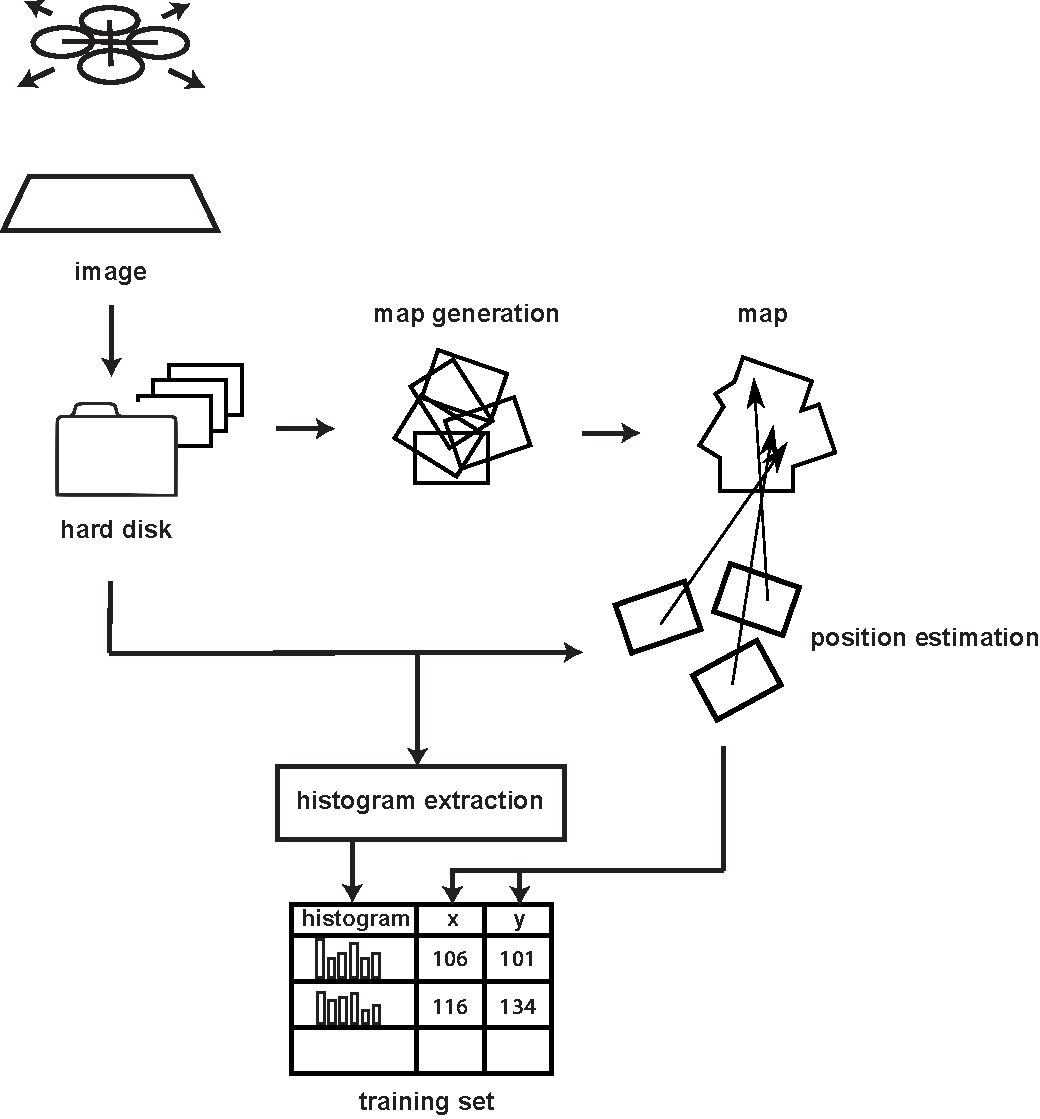
\includegraphics[width=0.7\columnwidth]{overview_sift}
\caption{{\label{fig:overview_sift} The figure illustrates the
    training set generation when applying the homography-based
    approach. Images from an initial flight are stitched together to
    create an orthomap. The same images are used to detect and
    describe their keypoints using \textsc{Sift}, followed by finding
    a homography between the keypoints of the flight images and the
    orthomap to obtain $x, y$-coordinates per image. The training set
    is created by extracting texton histograms from the images.
%inally, the $k$-NN algorithm uses the texton histogram as
%    feature vector and the corresponding $x, y$ coordinate as target
%    value. This process allows shifting computational burden of the
%    keypoint detection and homography finding to a faster machine
%    learning approach.%
  }}
\end{center}
\end{figure}

The stitching process can be time-consuming and error-prone. It can be
impeded by distortions and perspective transformations of the recorded
images. To circumvent the need for stitching together multiple images,
an image with a high-resolution camera from a top view point can be
taken that captures the entire area in some environments. Yet another
method starts with an existing image and modifies the environment
accordingly---for example by painting the floor or printing
posters--to correspond to the image.
%In all cases, we will describe
%the environment as \emph{map image}.
The homography-based process introduces noise into the dataset, since
it only has a limited accuracy (Section~\ref{sec:keypointmatching})
that depends on the quality of the keypoint matches.
% The $x,y$-positions are of different quality depending on the used
% technique: homography-based, poster-based, or motion tracking-based.
\begin{figure}[h!]
\begin{center}
\includegraphics[width=0.6\columnwidth]{bestmap}
\caption{{\label{fig:orthomap} This figure shows the created orthomap
    of a texture-rich floor. It is stitched together using 100 single
    images and represents a real world area of approximately
    $8\times8$ meters. Image distortions, non-mapped areas, and
    slightly skewed seams at several points are visible.%%
  }}
\end{center}
\end{figure}

%Instead of saving the images on the hard disk, the texton histograms
%can be directly aligned with the $x,y$-positions.

\section{Machine Learning-based Approach and Filtering}
\label{sec:textons}

In this section, the core of the developed algorithm is described: the
implementation of the texton framework, consisting of the texton
dictionary generation, the extraction of the histograms, the
$k$-Nearest Neighbors ($k$-NN) algorithm, and the particle filter. The
dictionary of textons constitutes the base for determining the texton
histograms. These histograms are used as features in the $k$-NN
algorithm. The algorithm outputs $k$ possible $x,y$-coordinates for a
given image, which are forwarded to the particle filter to yield a
final position estimation.

\subsection{Texton Dictionary Generation}
\label{sec:text-dict-gener}

For learning a suitable dictionary for an environment, image patches
were clustered. The resulting cluster centers---the prototypes of the
clustering result---are the textons~\cite{varma2003texture}. The
clustering was performed using a competitive learning scheme with a
``winner-take-all strategy,'' a simple variant of a Kohonen
network~\cite{kohonen1990self}. In the beginning, the dictionary is
initialized with $n = 20$ random image patches from the first image,
which form the first guess for cluster centers. Then, a new image
patch $x$ is extracted and compared to each texton $d_j$ in the
tentative dictionary using the Euclidean distance. The most similar
texton $d_r$ is the ``winner.'' This texton is then adapted to be more
similar to the current patch by calculating the difference in pixel
values between the current image patch and the texton and updating the
texton with a learning rate of $\alpha = 0.02$:
\begin{align*}
  d_r := d_r + \alpha (x - d_r)
\end{align*}
The first 100 images of each dataset were used to generate the
dictionary. From each image, 1\,000 randomly selected image patches of
size $w \times h = 6 \times 6$ pixels were extracted, yielding
$N = 100\,000$ image patches in total that were clustered. An example
of a learned dictionary of grayscale textons can be found in
Figure~\ref{fig:dictionary}. For our approach, we also used the color
channels U and V to obtain color textons.

Different maps and environmental settings require different texton
dictionaries. If one would use the same dictionary for each map, it
might happen that the histogram has only a few non-zero elements, and
thus, cannot represent the variance in the map. While we set the
number of textons to $n = 20$ for all maps, this parameter is also
map-dependent and should ideally be adapted to the given map.

\begin{figure}[h!]
\begin{center}
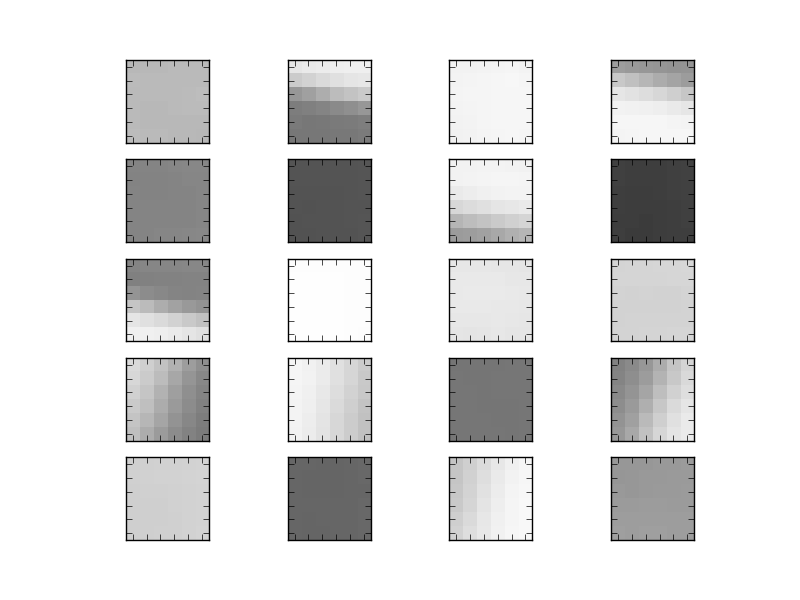
\includegraphics[width=0.7\columnwidth]{dict}
\caption{{\label{fig:dictionary} The figures shows a dictionary
    consisting of 20 grayscale textons ($w \times h = 6 \times 6$
    pixels).}}
\end{center}
\end{figure}

\subsection{Histogram Extraction}
\label{sec:histogramextract}

% TODO: Think if it is better here or in the related work section
%To extract histograms in the \emph{full sampling} setting, a small
%window---a kernel---is convolved over an image and the frequency of
%textons is calculated. 
%Instead of convolving a kernel over the entire
%image, the kernel can be applied at randomly sampled image
%position~\cite{de2012sub}.
The images from the preliminary dataset (Section~\ref{sec:mapping})
are converted to the final training set that consists of texton
histograms and $x,y$-values. It is the purpose of the conversion to
obtain a more representative and dense description of an image, which
should facilitate and speed-up recognition during the prediction
step~\cite{guyon2006introduction}. To extract histograms in the
\emph{full sampling} setting, a small window---or kernel---is
convolved across the width and height of an image and patches are
extracted from all positions. Each patch is compared with all textons
in the dictionary and is labeled with the nearest match based on
Euclidean distance comparing the pixels values in the channels Y, U,
and V. The frequency of each label is reported in the corresponding
``bin'' of the texton histogram. The histogram is normalized by
dividing the number of cases in each bin by the total number of
extracted patches, to yield the relative frequency of each texton.

The convolution is a time-consuming step, since all possible
combinations of width and height are considered:
$(640 - w + 1) \cdot (480 - h + 1) = 301\,625$ samples are
extracted. To speed up the time requirements of the histogram
extraction step, the kernel can be applied only to randomly sampled
image position instead~\cite{de2012sub}. This sampling step speeds up
the creation of the histograms and permits a trade-off between speed
and accuracy.
%The similarity between histograms in the full sampling
%step and the random sampling is analyzed in
%Section~\ref{sec:numtextons}.
One can see that the random sampling step introduces random effects
into the approach. Therefore, for generating the training dataset, no
random sampling was used to obtain high-quality feature vectors.

% The shift is accomplished by using a light-weight machine learning
% approach instead of a computationally more complex algorithm, like a
% homography-based approach (Section~\ref{sec:keypointmatching}).

\subsection{$k$-Nearest Neighbors ($k$-NN) algorithm}
\label{sec:knn}
% TODO: Write that one could also use a more efficient data structure than simply a list

The $k$-Nearest Neighbors ($k$-NN) algorithm is the ``machine
learning-core'' of the developed algorithm. Taking a texton histogram
as input, the algorithm measures the Euclidean distance of this
histogram to all histograms in the training dataset and outputs the
$k$ most similar training histograms and the corresponding
$x,y$-positions.

While the $k$-NN algorithm is one of the simplest machine learning
algorithms, it offers several advantages~\cite{kordos2010we}: it is
non-parametric, allowing for the modeling of arbitrary
distributions. Its capability to output multiple predictions enables
neat integration with the developed particle filter. Its simplicity
combines with transparency: it allows for spotting the possible
sources of error such as wrongly labeled training examples. $k$-NN
regression often outperforms more sophisticated
algorithms~\cite{knn}. A frequent point of criticism is its increasing
computational complexity with an increasing size of the training
dataset. While the used training datasets consisted of fewer than 1000
images, resulting in short prediction times, time complexity can be
reduced by storing and searching the training examples in an efficient
manner, for example, with tree structures~\cite{bhatia2010survey}.

% The similarity measure is a function that takes two samples as input
% and outputs a real value. We used the cosine similarity as
% similarity function, since it is bounded between 0 and 1. While
% other similarity measurements exists, the basic similarity
% measures---such as Euclidean distance---do not have a large impact
% on the results (Figure xxx). The choice of $k$ was based on the
% heuristic that XXX (TODO: write something like the sqrt of N or
% whatever) and on cross-validation.


\subsection{Filtering}
\label{sec:filtering}

Computer vision-based estimations are often noisy or ambiguous. Texton
histograms obtained during flight will not perfectly match the ones in
the training dataset: blur, lighting settings, viewing angles, and,
other variables change the shape of the histograms.

To filter out outliers and smooth estimates, a popular filter choice
is the Kalman filter. However, the Kalman filter is not able to
represent multimodal probability
distributions~\cite{dellaert1999monte}. This makes it rather
unsuitable for the presented \emph{global} localization approach. The
``naive'' $k$-NN regression calculates the mean of the $k$ outputs and
forwards this value to the Kalman Filter. However, if the output
values are distant, averaging them yields a value in the center
between them, which is not likely to be the correct position
(Figure~\ref{fig:kali}). This approach can lead to biased predictions,
especially, if the model outputs belong to distant locations due to
similar texton distributions at these positions.

\begin{figure}[h]
\begin{center}
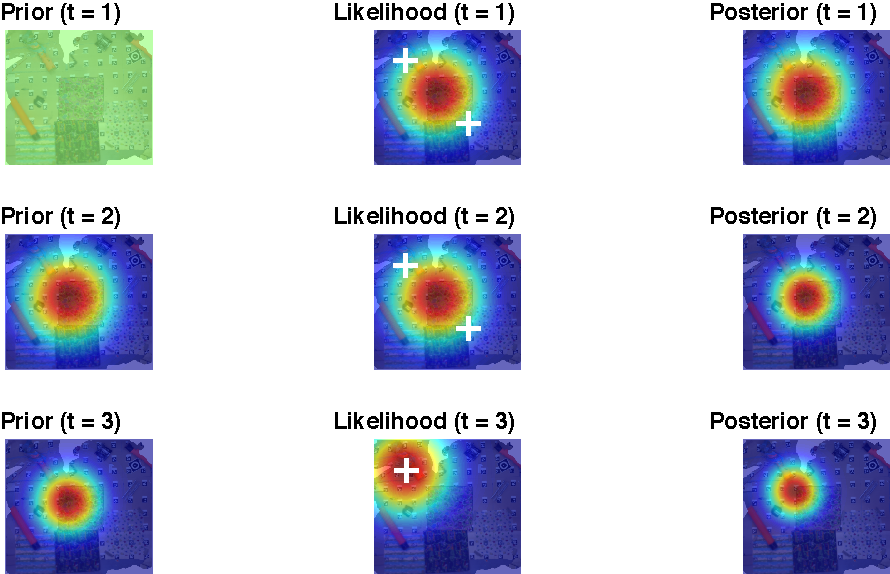
\includegraphics[width=0.8\columnwidth]{kalman-crop}
\caption[Kalman Filter.]{{\label{fig:kali} The figure illustrates the
    measurement model of a Kalman filter.  The colors represent the
    probability of an $x,y$-position (red: high probability; blue: low
    probability). In timestep $t = 1$, the filter is initialized with
    an uniformed prior and each position has equal probability.  To
    incorporate measurement error, the likelihood (measurement model)
    is calculated using a Gaussian distribution that is centered
    around the mean of the $k = 2$ predictions (white crosses) from
    the $k$-NN algorithm. The posterior results from the
    multiplication of the prior with the likelihood and indicates the
    position estimates after one timestep. In the next timestep, the
    previous posterior
  %  gets updated by introducing process noise and
    becomes the new prior.
    The filter receives distant measurements in time steps $t = 1$ and
    $t = 2$ that are averaged to receive a position in the middle. In
    time step $t = 3$, the ambiguity is resolved but the filter only
    slowly adapts to the new position.}}
\end{center}
\end{figure}

%Over time, however, the positional ambiguity, can be resolved, when
%both estimates of the $k$-NN model fall together. Compared to the
%Kalman filter, a full Bayesian filter could immediately find the
%correct position (Figure~\ref{fig:bayesianfilter}). Since a full
%Bayesian filter is computationally complex, a variant that is based on
%Monte Carlo sampling was used: the particle filter. A detailed
%description of the filtering technique can be found in the next
%section.

We decided to use a more sophisticated method to capture
\emph{multimodal distributions}. Given an adequate measurement model,
a general Bayesian filter can simultaneously maintain multiple
possible locations and resolve the ambiguity as soon as one location
can be favored (Figure~\ref{fig:bayes}). In this case, the predictions
of the $k$ neighbors can be directly fed into the filter without
averaging them first. The filter is able to smooth the estimations,
handle uncertainty, and simultaneously keep track of several position
estimates. However, a general Bayesian filter is computationally
complex. Therefore, a variant based on random sampling was used: the
particle filter. While its computational complexity is still high
compared to a Kalman filter, one can modify the amount of particles
to trade off speed and accuracy and adapt the computational payload to
the used processor.


\begin{figure}[h]
\begin{center}
  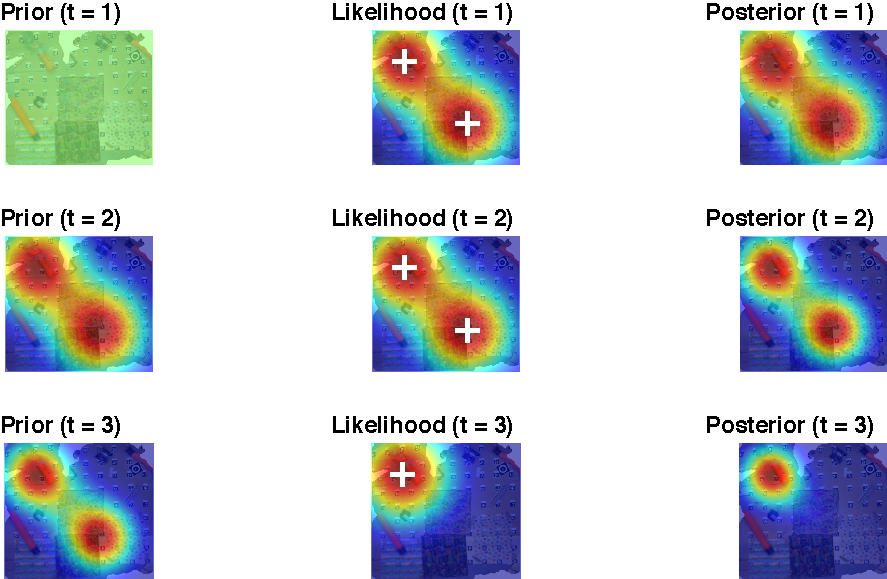
\includegraphics[width=0.8\columnwidth]{particle-crop}
  \caption[Bayesian Filter.]{{\label{fig:bayes} Three time steps of a
      Bayesian filter. The colors represent the probability of an
      $x,y$-position (red: high probability; blue: low
      probability). In contrast to the Kalman filter, the likelihood
      (measurement model) is calculated using a \emph{mixture} of
      Gaussian distributions centered around the outputs the $k$-NN
      algorithm (white crosses). The filter can immediately resolve
      the ambiguity in time step 3 and the posterior gets updated
      accordingly.}}
\end{center}
\end{figure}


The weighted particles are a discrete approximation of the probability
density function ($pdf$) of the state vector ($x,y$-position of the
MAV). Estimating the filtered position of the MAV can be described as
$p(X_t \mid Z_t)$, where $X_t$ is the state vector at time $t$ and
$Z_t = \mathbf{z}_1, ..., \mathbf{z}_t$ are all outputs of the $k$-NN
algorithm up to time $t$, with each $\mathbf{z}_i$ representing the
$k$ $x,y$-outputs of the algorithm at time $i$.
% The state vector is \emph{hidden}, since the variables cannot be
% measured directly, therefore the situation can be described with a
% hidden Markov model.  Instead, noisy or ambiguous data can be
% obtained through the proposed algorithm.


The used particle filter is initialized with $M = 100$ particles at
random $x, y$-positions. To incorporate the measurement noise for each
of the $k$ estimates from the $k$-NN algorithm, we developed a
two-dimensional Gaussian Mixture Model (GMM) as measurement model. The
parameters of the GMM are obtained by comparing the ground truth
positions (random variable $T$) from the motion tracking system to the
estimates from the $k$-NN algorithm (random variable $P_j$) in a
recorded dataset. The GMM is parameterized by the
variances~$\Sigma^{[j]}, j \in \{1, \ldots, k\}$ that are dependent on the
rank $j$ of the prediction of the $k$-NN algorithm (for example,
$j = 2$ is the second nearest neighbor).
%The value $\mu_j$ represents
%the average deviation from the ground truth for the $j$th prediction
%of the $k$-NN algorithm;
The variance matrix $\Sigma^{[j]}$ specifies the variances of the
deviations in $x$-direction and $y$-direction and the correlation
$\rho$ between the deviations.
%$p(z \mid x) = \frac{p(x \mid z)p(z)}{p(x)}$ is used, where
%$\textbf{x} = ((x_1, y_1), (x_2, y_2), \ldots, (x_k, y_k))^T$. A
%a two-dimensional Gaussian sensor model was used for each resulting in
%a Gaussian Mixture Model.
The values for $\Sigma^{[j]}$ were determined by calculating the
variance-covariance matrix for the difference between the ground truth
$T$ and the predictions $P_j$ of the $k$-NN algorithm:
$\Sigma^{[j]} := \text{Var}(T-P_j)$.

In contrast to the measurement model, the used \emph{motion model} is
simple. It is solely based on Gaussian process noise and does not
consider velocity estimates, headings, or control inputs. Its mean and
variance are dependent on the expected velocity of the MAV. We used
the forward difference $T_t - T_{t-1}$ to estimate the average
movement and its variance-covariance matrix $\Sigma_{\text{process}}$
between timesteps $t$ and $t-1$. While the employed motion model is
simple, the developed software provides functionality for including an
odometry-based motion model based on optical flow.

The algorithm of the developed particle filter is presented in the
pseudo code in Algorithm~\ref{alg:particle_filter}. In the pseudo
code, $\mathcal{X}$ is the list of particles, $f$ the two-dimensional
Gaussian probability density function, $z_t^{[i]}$ the $i$th neighbor
from the $k$NN prediction, $x_t^{[m]}$ the $m$th particle at time $t$,
and $w_t^{[m]}$ its corresponding weight.
\begin{algorithm}
\caption{Particle filter update}
\label{alg:particle_filter}
\begin{algorithmic}[1]
  \Procedure{Particle\_Filter}{$\mathcal{X}_{t-1}, z_t$}
    \LineComment Initialize particle list
  \State $\mathcal{X}_{\text{temp}} := \varnothing$
  %\Comment $q$ is process noise, $r$ is measurement noise
  %\State $q_x^2 = 15$, $q_y^2 = 15$, $r_x^2 = 100$, $r_y^2 = 100$
  \For{$m = 1$ to $M$}
  \LineComment{Add random process noise (motion model)}
  \State $x_t^{[m]} \gets x_t^{[m]} + \mathcal{N}(0, \Sigma_{\text{process}})$
  \LineComment{Iterate over predictions from $k$-NN (measurement model)}
  \State $w \gets 0$
  \For{$i = 1$ to $k$}
      % p = binormpdf(xs[i].x, xs[i].y, z[pred].x, z[pred].y,
      %               measurement_noise_x, measurement_noise_y, rho);
      % total_likelihood $\gets$ total_likelihood;
  %     \State sample $x_t^{[m]} \sim \mathcal{N}(x_{t-1}^{[m]},
   %    q_x^2)$
  %\State $x_t^{[m]} \sim \mathcal{N}(x_{t-1}^{[m]}, q_x^2)$ \State
  \LineComment{Gaussian Mixture Model}
  \State $w \gets w + f(z_t^{[i]} ; x_t^{[m]}, \Sigma_{\text{measurement}}^{[i]})$ 
       \EndFor
  \State $\mathcal{X}_{\text{temp}} := \mathcal{X}_{\text{temp}} \cup  (x_t^{[m]}, w)$
%  \State sample $y_t^{[m]} \sim \mathcal{N}(y_{t-1}^{[m]}, q_y^2)$
  % Resampling wheel
  \EndFor
  \LineComment{Importance resampling}
%  \State $\mathcal{X}_t \gets$
  \State $\mathcal{X}_t \gets$ \Call{Resampling\_Wheel}{$\mathcal{X}_{\text{temp}}$}
  \State \Return $\mathcal{X}_t$
  \EndProcedure
\end{algorithmic}
\end{algorithm}

The ``resampling wheel''~\cite{thrun}
(Algorithm~\ref{alg:resampling_wheel}) performs the importance
resampling step. Its underlying idea is that the particles are
arranged in a ``wheel,'' with each particle occupying a slice that
corresponds to its weight. The particles are then resampled with a
probability proportional to the area of the slices. This step ensures
that particles with a low weight are removed and replaced with
well-performing ones. Otherwise, the algorithm might ``collapse'' when
all but one particle have a low weight.

\begin{algorithm}
\caption{Resampling wheel}
\label{alg:resampling_wheel}
  \begin{algorithmic}[1]
    \Procedure{Resampling\_Wheel}{$\mathcal{X}_{\text{temp}}$}
    \LineComment Initialize particle list
    \State $\mathcal{X}_t \gets \emptyset$
    \LineComment Sample random index from the number of particles
    \State sample $i \sim M \cdot \mathcal{U}(0, 1)$
    \State $\beta \gets 0$
    \For{$m = 1$ to $M$}
    \State $\beta \gets \beta + \mathcal{U}(0, 1)\cdot 2\cdot \max(w_t)$
    \While{$\beta > w_t^{[i]}$}
    \State $\beta \gets \beta - w_t^{[i]}$
    \State $i \gets (i + 1) \mod M$
    \EndWhile
    \State $\mathcal{X}_t \gets \mathcal{X}_t \cup \mathcal{X}_{\text{temp}}^{[i]}$
    \EndFor
  \State \Return $\mathcal{X}_t$
\EndProcedure
\end{algorithmic}
\end{algorithm}

%The mean values $\mu$ were set to zero (no systematic
%bias).
%(Figure~\ref{fig:measurementmodel}).


%\begin{figure}
%  \label{fig:cor_sim_confi}
%  \centering
%  \begin{subfigure}[b]{0.5\textwidth}
%  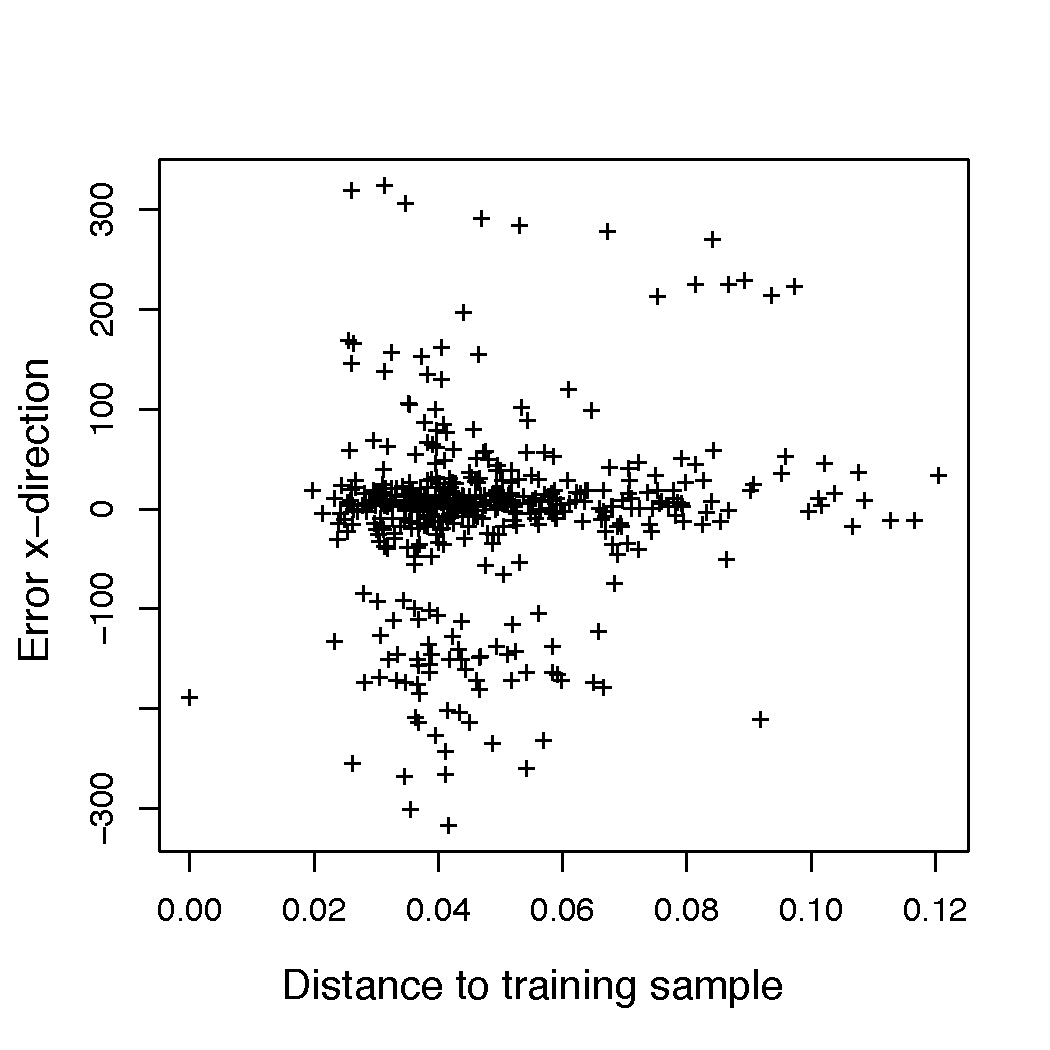
\includegraphics[width=1\textwidth]{dependency_dist_error_x}
%    %\captionof{figure}{$POS_x$}
%  \label{fig:cosinesim}
%  \end{subfigure}%
%~
%  \begin{subfigure}[b]{0.5\textwidth}
%  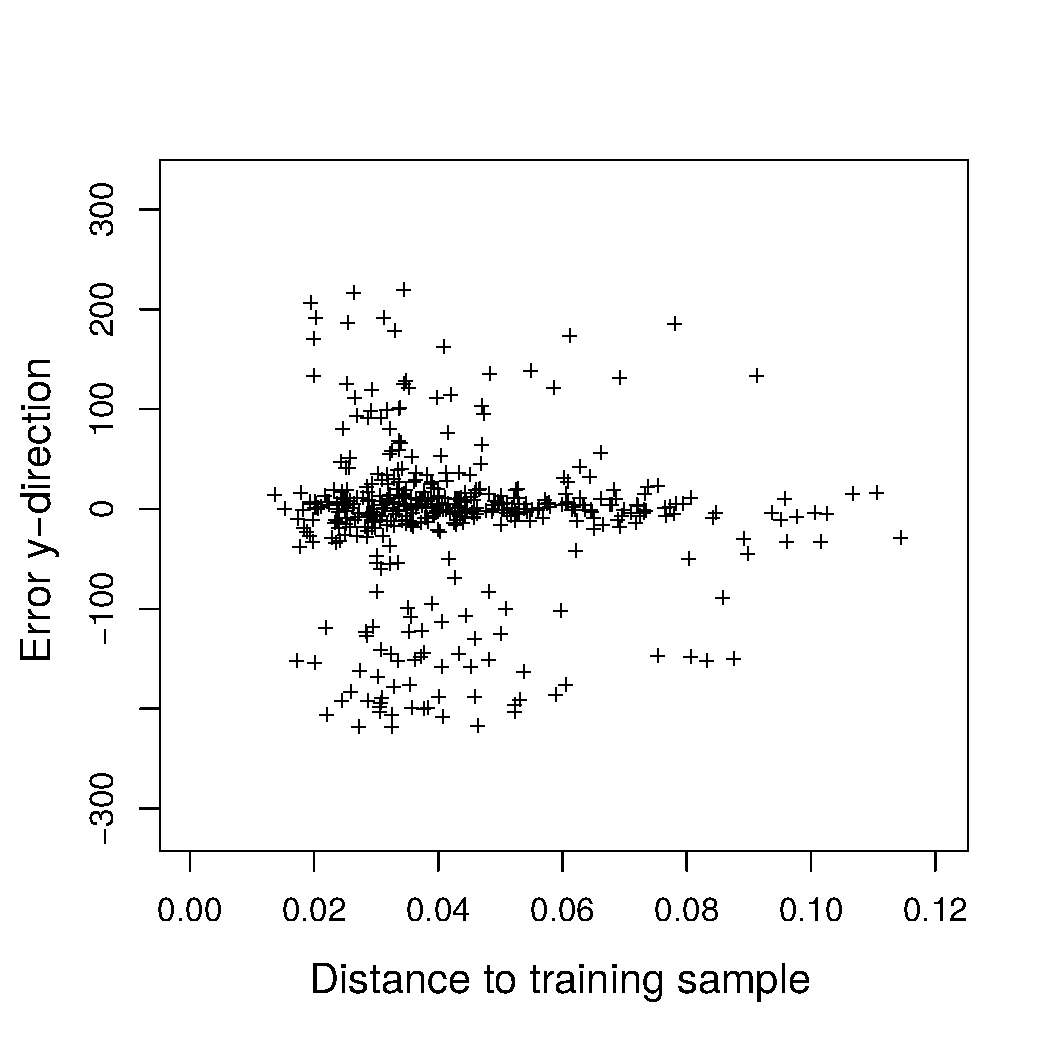
\includegraphics[width=1\textwidth]{dependency_dist_error_y}
%   % \captionof{figure}{$POS_y$}
%  \label{fig:cosinesd}
%  \end{subfigure}
%  \caption{Measurement error in $x$-direction (\emph{Left}) and
%    $y$-direction (\emph{Right}) as a function of the distance to the
%    closest training sample.}
%\label{fig:cosine}
%\end{figure}
%\unsure{uiui, should edit the labels of the y axis and uses crosses in
%both cases}
%\begin{figure}[h!]
%\label{fig:measurementmodel}
%\begin{center}
%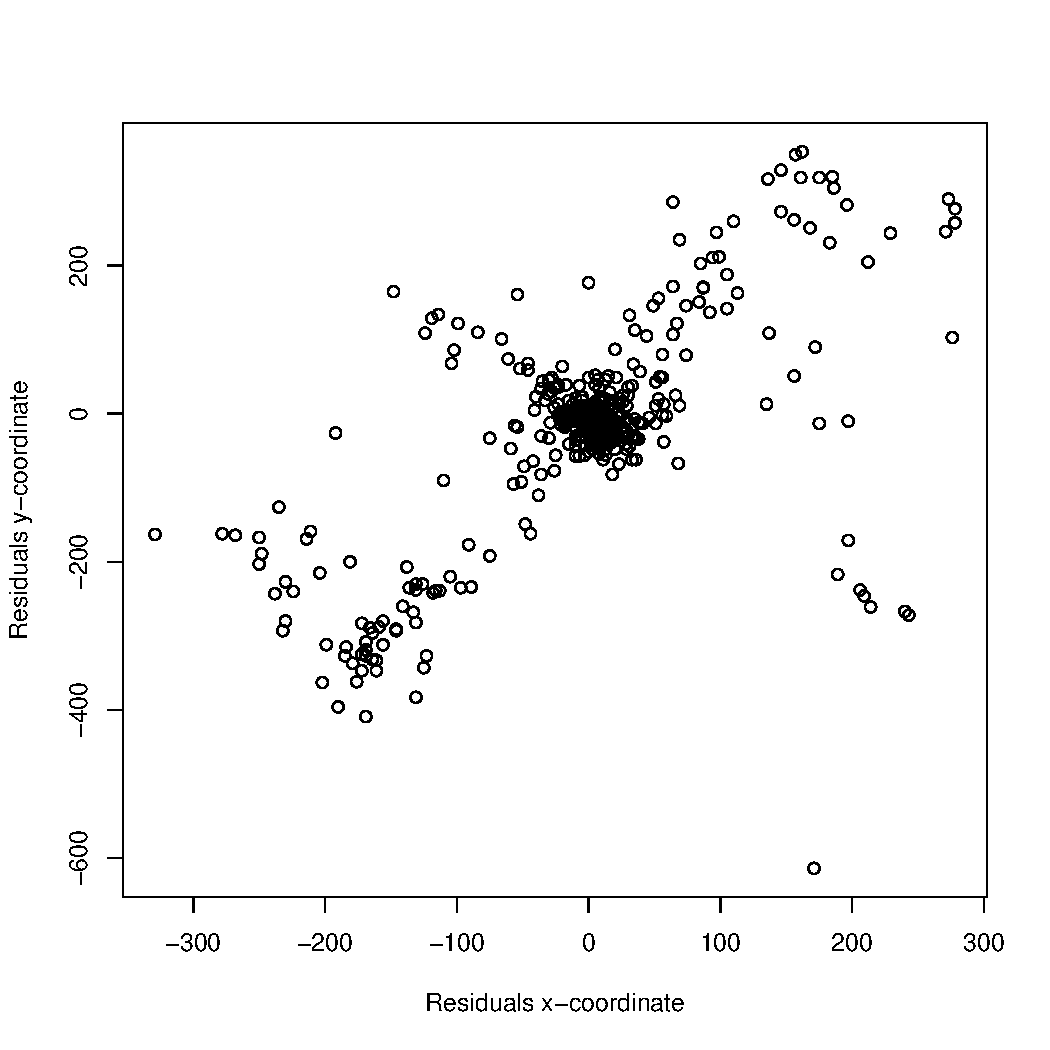
\includegraphics[width=0.448\columnwidth]{measurement_model}
%\caption{{Measurement model showing the delta x and delta y positions.
%  }}
%\end{center}
%\end{figure}
%\unsure{TODO: Add Gaussian approximation!}
With the GMM, the information of all $k$ neighbors can be used,
yielding a possibly multimodal distribution. While a multimodal
distribution allows for keeping track of several possible positions,
certain subsystems---for example a control loop---often need
\emph{one} point estimate. Using a weighted average of the particles
would again introduce the problem that it could fall into a low
density region (an unlikely position). Instead, we used a maximum a
posteriori (MAP) estimate, as described by
\citeauthor{driessen2008map}~\cite{driessen2008map}. This approach is
a discrete approximation of the true MAP~\cite{driessen2008map}. It
uses the following formula to obtain the MAP estimate
$X_t^{\text{MAP}}$---the ``final'' $x,y$-position:
\begin{align*}
X_t^{\text{MAP}} = \argmax_{x_t^{[i]} \in \{i=1,\ldots,M\}} \sum_{j =
  1}^{M}f(x_t^{[i]} ; x_{t-1}^{[j]},\Sigma_{\text{process}})w_{t-1}^{[j]}
\end{align*}
Therefore, the final position estimate is equal to the position of one
of the particles.

The estimation of \emph{uncertainty} is a core part of the developed
approach, due to its importance for safety and accuracy. Therefore,
uncertainty was modeled using the spread of the particles---as
expressed by their variance in $x$-direction and $y$-direction.
%These estimates are noisy, as illustrated
%in Figure~\unsure{TODO: add edgeflow noisea add fig:edgeflow}:
%Optical flow estimates accumulate errors over time. 
%the outputs of the $k$-NN algorithm are independent of previous
%predictions. Therefore, the predictions could `jump' to locations due
%to prediction errors. The particle filter is used to combine the
%advantages of both methods and eliminate the disadvantages.
Initially, we planned to include the distance between the current
histogram obtained from the camera image and each of the $k$ neighbors
from the training set as confidence value. One could thus reduce the
measurement noise if a high similarity between the current histogram
and a training histogram is achieved. While we found no correlation
between these variables, we still provide the
functionality for incorporating the distance in the developed
software.
% (Figure~\ref{fig:cor_sim_confi})
We also tried to use the amount of detected keypoints ($K$) as a
confidence value for the quality of the sample in the training set if
the homography-based approach is used for labeling. Again, no linear
relationship between $K$ and the error in $x$-direction ($X$) and the
error in $y$-direction ($Y$) could be found.
%(Figure~\ref{fig:cor_keypoints})
%: $\rho_{K, X} = 0.10$,
%$\rho_{K, Y} = 0.01$.

%\begin{figure}
%  \label{fig:cor_keypoints}
%  \centering
%  \begin{subfigure}[b]{0.5\textwidth}
%  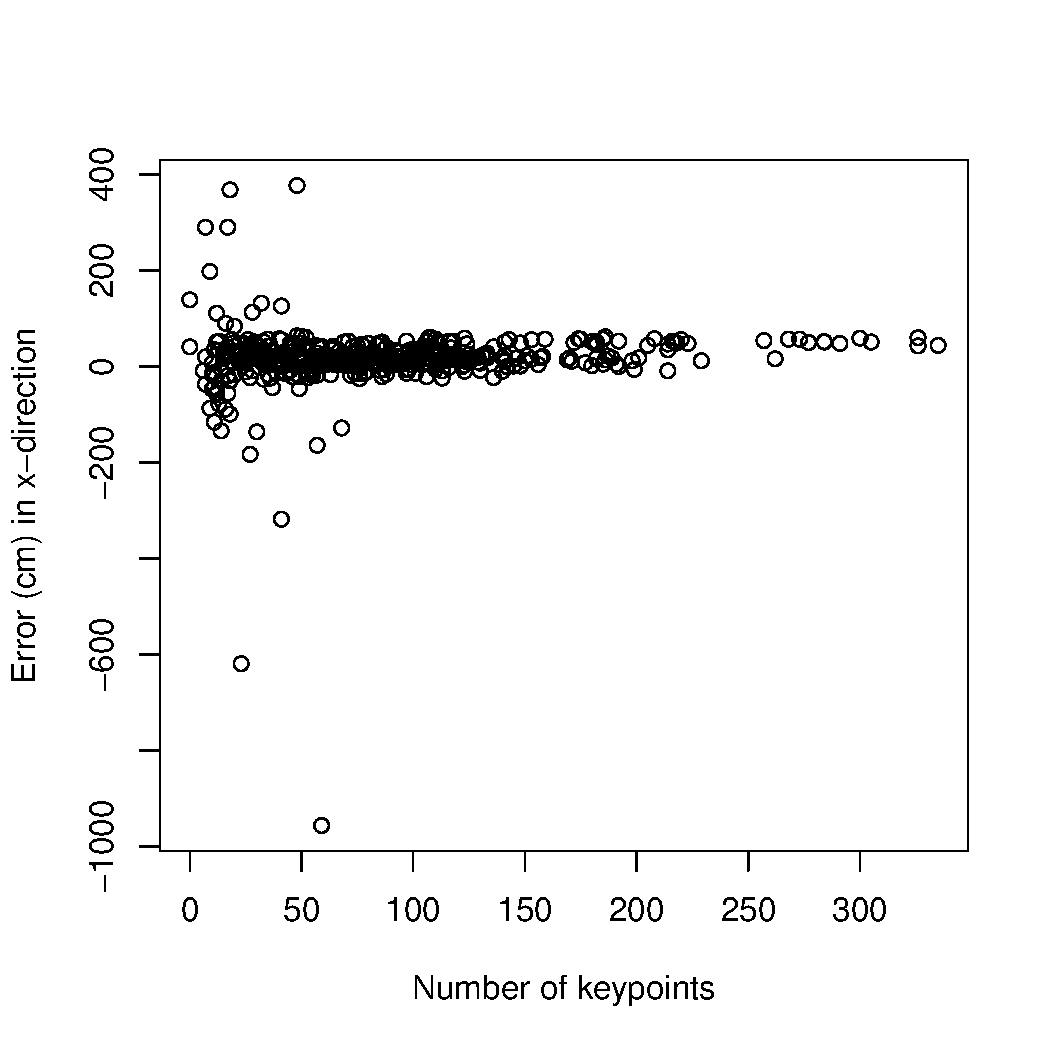
\includegraphics[width=1\textwidth]{keypoints_error_x1}
%    %\captionof{figure}{$POS_x$}
%  \label{fig:cosinesim}
%  \end{subfigure}%
%~
%  \begin{subfigure}[b]{0.5\textwidth}
%  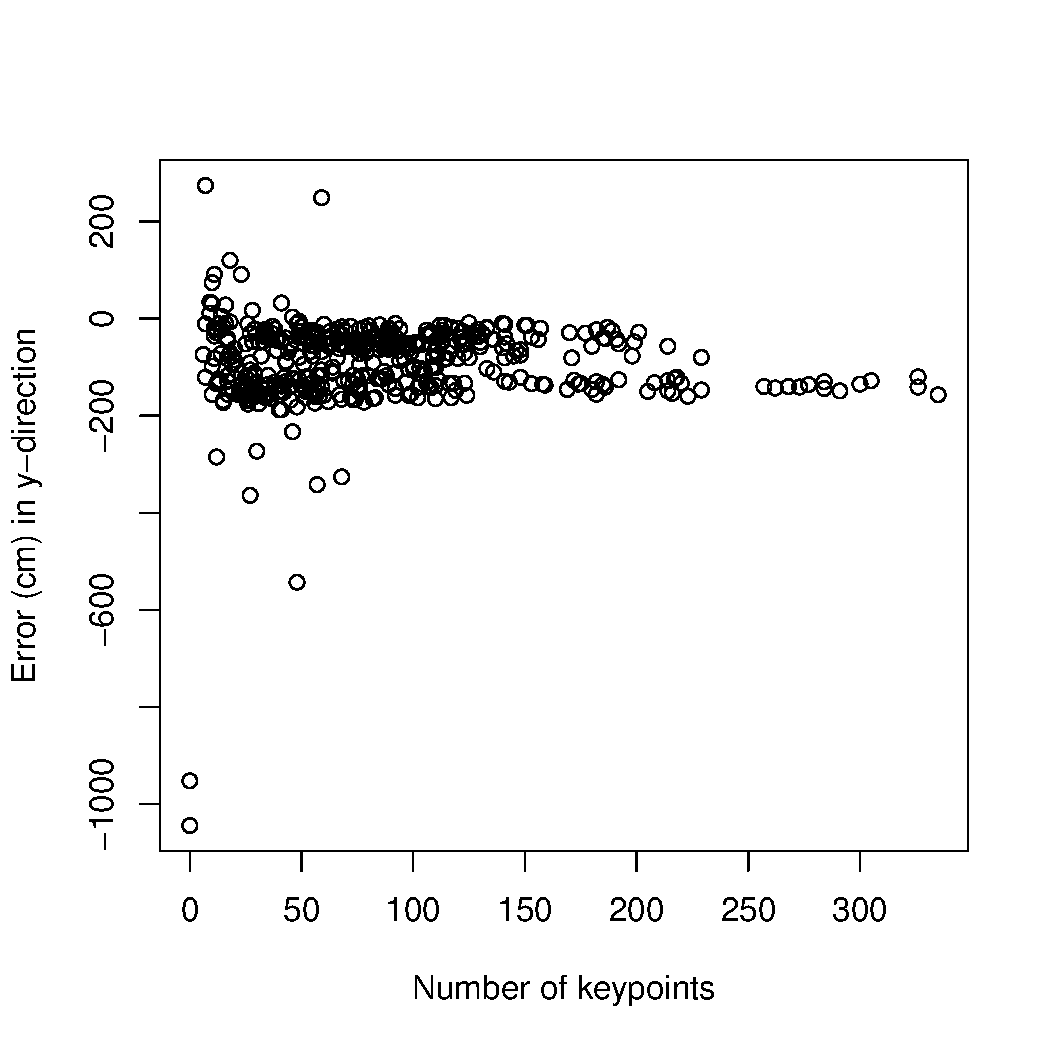
\includegraphics[width=1\textwidth]{keypoints_error_y}
%   % \captionof{figure}{$POS_y$}
%  \label{fig:cosinesd}
%  \end{subfigure}
%  \caption{Measurement error in $x$-direction (\emph{Left}) and
%    $y$-direction (\emph{Right}) as a function of the number of
%    keypoints found by \textsc{Sift}.}
%\label{fig:cosine}
%\end{figure}
%
%\unsure{uiui, should edit the labels of the y axis and uses crosses in
%both cases}

%

\section{Map evaluation}
\label{sec:mapeval}

\subsection{Evaluation Scheme}
\label{sec:evaluationscheme}

The performance of the developed method depends on the environment: a
texture-rich environment without repeating patterns will be better
suited than a texture-poor environment. Ideally, one would like to
know if the algorithm will work in a given environment. Therefore, we
propose an evaluation scheme that can compare different environments
and areas within an environment. This scheme assigns a global fitness
value to a ``map''---expressed as dataset $\mathcal{D}$ consisting of
$N$ texton histograms $h_i$ and corresponding $x,y$-coordinates
$\text{pos}_i = (x_i, y_i)$. The fitness value is proportional to the
accuracy that can be expected when using this dataset as training set
for the developed localization algorithm. The scheme allows for
inspecting the dataset and detecting regions within the map that are
responsible for the overall fitness value.
%The
%evaluation of a map is difficult, since the obtained histograms during
%a real flight depend on many factors: motion blur, distance to the map
%and rotations proportional to the map.

The idea behind the global loss function $L$ is that histograms $h_i$
and $h_j$ in closeby areas should be similar and the similarity should
decrease with increasing distance of the corresponding
$x,y$-coordinates $\text{pos}_i$ and $\text{pos}_j$. Therefore, the
approach is based on the difference between \emph{actual} and
\emph{ideal} texton histogram similarities in a dataset. The ideal
texton similarity distribution is modeled as a two-dimensional
Gaussian distribution around each $x,y$-position in the dataset
(Figure~\ref{fig:local_loss}). Using this idea, a histogram is
compared to all others by comparing expected similarities to actual
similarities. This results in a loss value per sample of the
dataset. Applying the algorithm to each sample in the dataset yields
the global loss of a dataset. A visualization of the global loss is
illustrated in Figure~\ref{fig:globalloss}.

\begin{figure}[h!]
\begin{center}
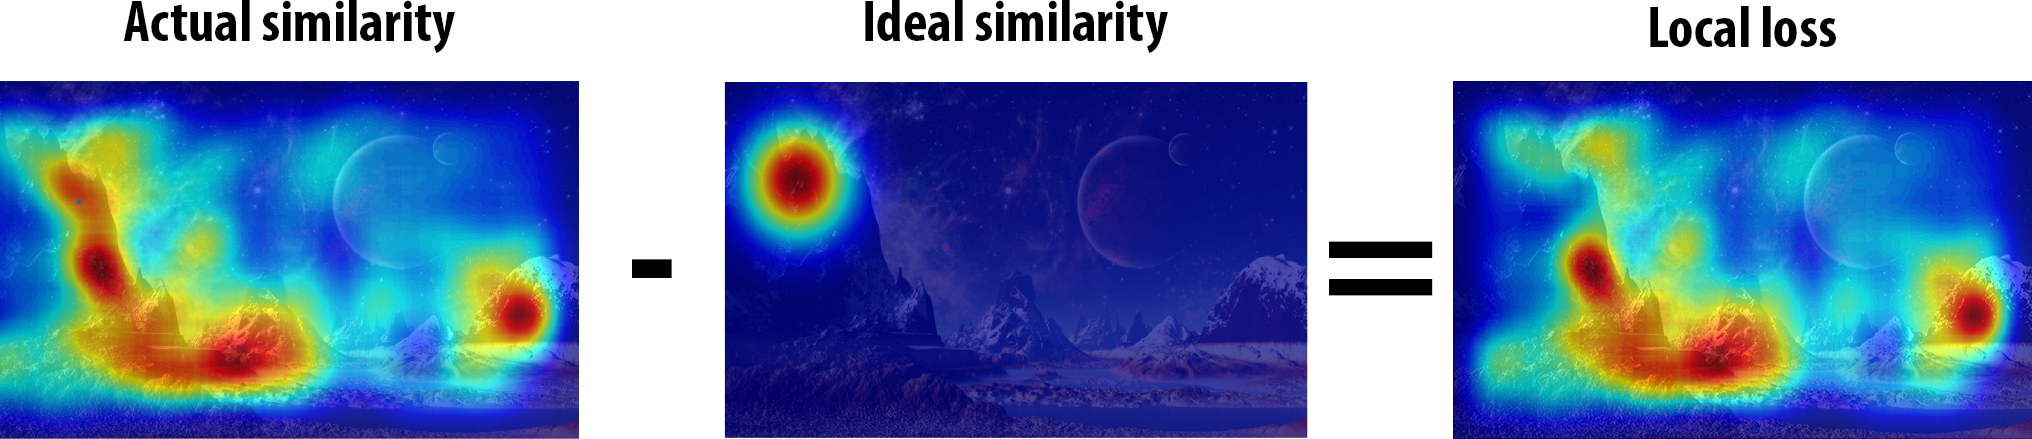
\includegraphics[width=1\columnwidth]{local_loss}
\caption{{\label{fig:local_loss}\emph{Left:} Actual similarity between
    histogram $h_i$ ($\text{pos}_i$: white cross) and all other
    histograms; the heatmap shows low similarity in blue and high
    similarity in red.  For the visualization, the actual similarities
    were smoothed with a Gaussian filter. \emph{Middle:} Ideal
    histogram similarity distribution for the given position
    $\text{pos}_i$. Histograms $h_j$ taken at closeby positions should
    have a high similarity to $h_i$. The farther away the position
    $\text{pos}_j$, the lower the similarity between $h_i$ and $h_j$
    should be. \emph{Right:} The difference between the actual and the
    ideal similarity shows regions that do not follow the ideal
    similarity distribution for histogram $h_i$ (high loss: red; low
    loss: blue)}}
\end{center}
\end{figure}

The method uses the cosine similarity ($CS$) to compare histograms:
\begin{align*}
CS(h_i, h_j) = \frac{h_i^Th_j}{||h_i||\,||h_j||}
\end{align*}
The cosine similarity has the convenient property that its values are
bounded between $-1$ and $1$. In the present case, since the elements
of the histograms are non-negative, it is even bounded between $0$ and
$1$. Let the function $f$ describe the non-normalized one-dimensional
Gaussian probability density function:
\begin{align*}
  f(x; \mu, \sigma) = e^{- \frac{(x - \mu)^2}{2 \sigma ^ 2}}  
\end{align*}
Since we assume that the ideal similarity in $x$-position is
independent of the $y$-position, the ideal two-dimensional similarity
function $d_e(\text{pos}_i, \text{pos}_j; \Sigma)$ can be modeled as
the product of the respective one-dimensional function~$f$:
\begin{align*}
d_e(\text{pos}_i, \text{pos}_j; \Sigma) = f(x_i; x_j, \sigma_x) \cdot f(y_i;
y_j, \sigma_y)
\end{align*}
This function is also bounded between $0$ and $1$, which makes the
functions $d_e$ and $CS$---ideal similarity and actual
similarity---easily comparable. In summary, we propose the following
global loss function ($L$) for evaluating a given dataset
($\mathcal{D}$):
\begin{align*}
  L(\mathcal{D}) &= \frac{1}{N^2}\sum_{i = 1}^{N} \sum_{j = 1}^{N}
                   CS(h_i, h_j) - f(x_i; x_j, \sigma_x) \cdot f(y_i; y_j, \sigma_y)                  
\end{align*}
The simple difference---in contrast to least absolute deviations or
least square errors---ensures that similarities that are \emph{less}
similar than the ideal similarity \emph{reduce} the loss. Therefore, a
high variation in texture is always seen as ``positive''. The
variances $\sigma_x$ and $\sigma_y$ specify the dimension of the
region, where similar histograms are desired. The lower their value,
the more focused the ideal similarity will be, requiring a high
texture variety for getting a low loss value. A high value might
overestimate the suitability of a dataset. While the approach is
relatively robust to the choice of the parameter values, we still need
to find a heuristic for suitable values.
\begin{figure}[h]
  \centering
  \includegraphics[width=\textwidth]{global_loss-crop}
  \caption{The figure shows the loss of a map: the regions that did
    not follow the ideal similarity pattern are displayed in red. For
    the visualization, the loss values per sample in the dataset were
    smoothed with a Gaussian filter. This assigns a loss value to each
    $x,y$-position of the map. The synthetic data generation tool was
    used for generating the underlying dataset
    (Section~\ref{sec:syntheticdatageneration}). }
  \label{fig:globalloss}
\end{figure}

%\unsure{TODO: look what a cap with max(dist, 0) would do; look also
%  into it, if we need an absolute value function; maybe the minus is
%  already better than a cap}


\subsection{Synthetic Data Generation}
\label{sec:syntheticdatageneration}

To compare environments before actually flying in them, a software
tool was developed that creates synthetic images to simulate those
taken during an actual flight.
%In the scope of this thesis, an application to simulate different
%camera positions during flight was created.
The tool generates the patches based on perspective transformations of
an image. Examples of generated images are displayed in
Figure~\ref{fig:montage}.

\begin{figure}[h]
\begin{center}
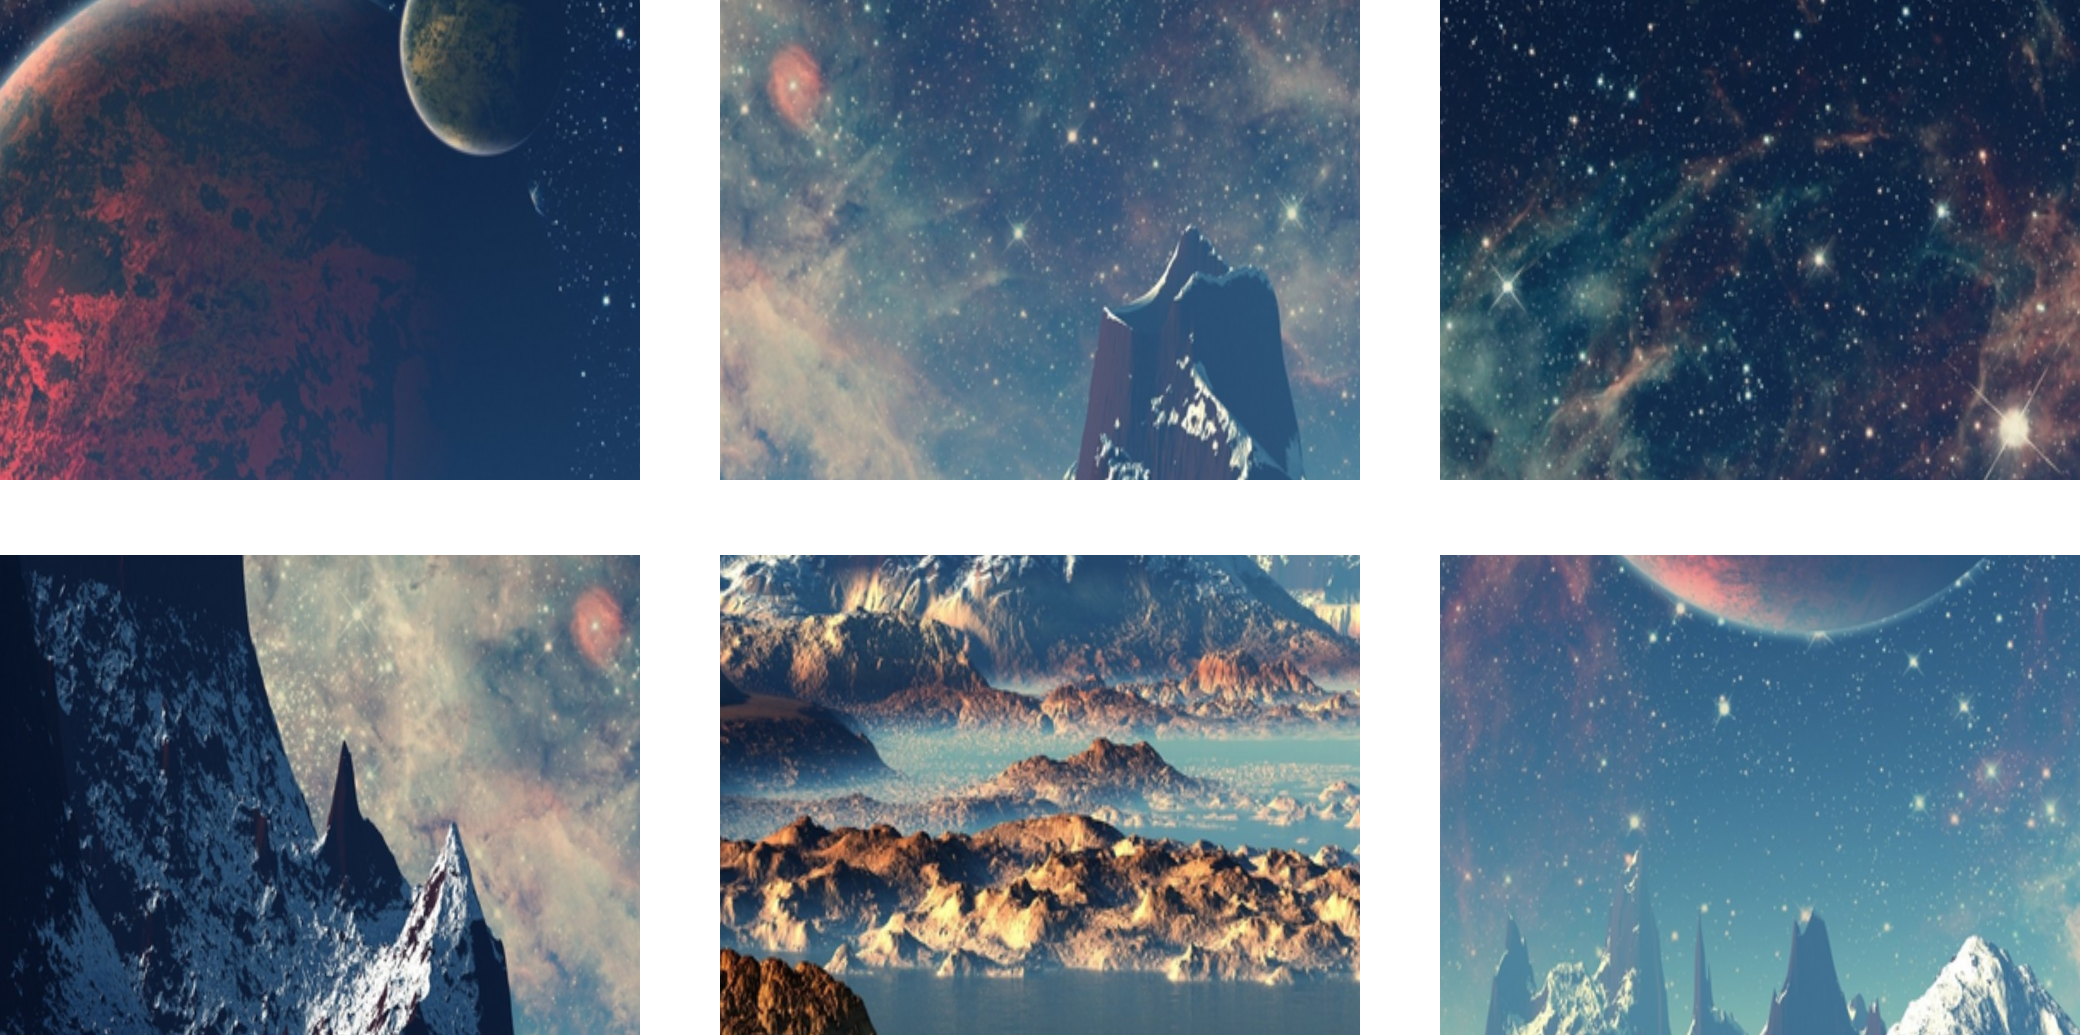
\includegraphics[width=0.7\columnwidth]{samples}
\caption{{\label{fig:montage} 
Six image patches generated by means of the synthetic data generation tool.%
}}
\end{center}
\end{figure}

The application allows for comparing and predicting the performance of
different ``maps'' as specified by an image. The software is written
in C++ and OpenCV~3.0.0. 
The algorithm simulates a simple camera model that moves above the
image (Figure~\ref{fig:cammodel}).
It generates a specified amount of image
patches using random values---sampled from uniform and normal
probability distributions---for various parameters:
\begin{itemize}
\item rotational angles: roll $\alpha$, pitch $\beta$, yaw
  $\gamma$
\item translational shifts: d$x$, d$y$, d$z$
\item brightness: addition of constant value $b$ to all pixels
\item contrast: multiplication of pixel values with constant value $c$
\item blur: application of a box filter with kernel size
  $kw \times kh$
\end{itemize}

By finding a homography $M$---a perspective transformation specified
by rotational and translational parameters---one can obtain image
patches and consequently texton histograms to create a training
dataset. The tool labels the generated patches with the corresponding
simulated $x,y$-position of the camera model, which represents the
position of the UAV.

\begin{figure}[h]
\begin{center}
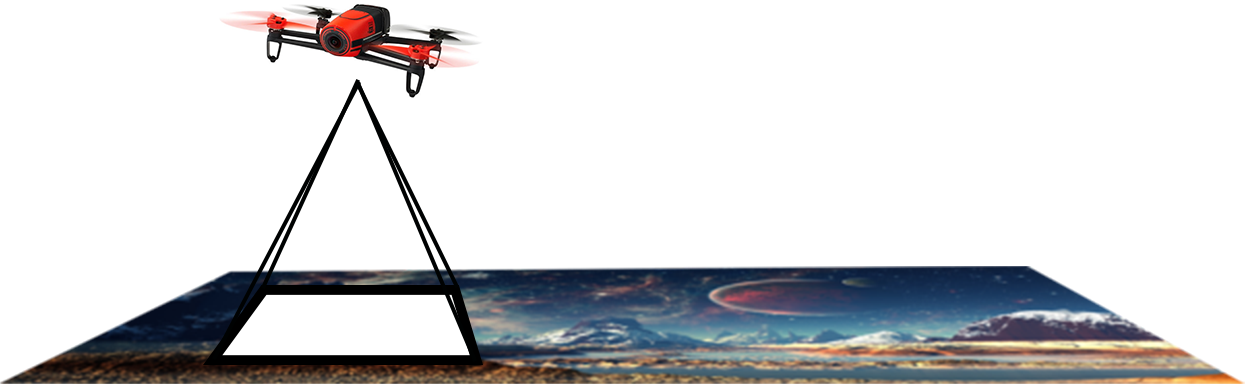
\includegraphics[width=0.672\columnwidth]{camera_model}
\caption{{\label{fig:cammodel} Illustration of the camera model for
    the synthetic flight. The developed tool extracts image patches
    from an given image to simulate those taken with the bottom camera
    of the MAV during an actual flight.}}
\end{center}
\end{figure}
The steps for specifying the homography are outlined in the
following. The implementation is partly based on work by
\citeauthor{jepson}~\cite{jepson}. \citeauthor{hartley2003multiple}~\cite{hartley2003multiple}
describe multiple view geometry and image transformations in computer
vision in detail.  To simulate camera movements in the 3D world, a 2D
to 3D projection of the image is performed first, using the matrix
$P_3$, with the width~$w$ and height~$h$ of the image:
\begin{align*}
  P_3 = \begin{bmatrix}
  1             & 0            & -\frac{w}{2}      \\
  0             & 1            & -\frac{h}{2}      \\
  0             & 0            & 0                 \\
  0             & 0            & 1                 \\
  \end{bmatrix}
\end{align*}
The result is a 3D space with the center of the image as point of
origin. The camera rotations are specified by the rotation matrix
$R = R_x \cdot R_y \cdot R_z$. By building rotation matrices $R_x$,
$R_y$, and $R_z$ around the axes $x$, $y$, and $z$, the rotations with
the corresponding angles $\alpha, \beta$, and $\gamma$ can be defined
separately:
\begin{align*}
R_x = 
  \begin{bmatrix}
  1             & 0            & 0             & 0 \\
  0             & \cos(\alpha) & -\sin(\alpha) & 0 \\
  0             & \sin(\alpha) & \cos(\alpha)  & 0 \\
  0             & 0            & 0             & 1 \\  
  \end{bmatrix}
\end{align*}
\begin{align*}
  R_y = 
  \begin{bmatrix}
    \cos(\beta) & 0            & -\sin(\beta)  & 0 \\
    0           & 1            & 0             & 0 \\
    \sin(\beta) & 0            & \cos(\beta)   & 0 \\
    0           & 0            & 0             & 1 \\
      \end{bmatrix}
\end{align*}
\begin{align*}
  R_z =
  \begin{bmatrix}
  \cos(\gamma)    & -\sin(\gamma)  & 0             & 0 \\
  \sin(\gamma)    & \cos(\gamma)   & 0             & 0 \\
  0             & 0            & 1             & 0 \\
  0             & 0            & 0             & 1 \\
      \end{bmatrix}
  \end{align*}

  The 3D translational matrix $T$ specifies the location of the camera
  in world coordinates:
\begin{align*}
  \tilde{T} = \begin{bmatrix}
    1 & 0 & 0 & \text{d}x        \\
    0 & 1 & 0 & \text{d}y        \\
    0 & 0 & 1 & \text{d}z        \\
    0 & 0 & 0 & 1        \\
  \end{bmatrix}
\end{align*}
Now, a rotation followed by translation can be specified by matrix
$H$:
\begin{align*}
  H = T \cdot R
\end{align*}
However, this matrix $H$ describes how the world is transformed
relative to the camera coordinates, while the position of the camera
is fixed. Instead, we would like to specify the camera movement
relative to a fixed world. To this end, the inverse of $H$ is needed:
\begin{align*}
  H' = (T \cdot R)^{-1} = R^{-1} \cdot T^{-1}
\end{align*}
The transposed rotation matrix is equal to its inverse: $R' =
R^{-1}$. The inverse of $T$ negates the translations:
\begin{align*}
  T^{-1} = \begin{bmatrix}
  1 & 0 & 0 & -\text{d}x        \\
  0 & 1 & 0 & -\text{d}y        \\
  0 & 0 & 1 & -\text{d}z        \\
  0 & 0 & 0 & 1        \\
  \end{bmatrix}
\end{align*}
To obtain a 2D image again, a projection from 3D space to 2D is
applied using the matrix $P_2$. The matrix needs the focal distance
$f$ (the distance between camera and image).
\begin{align*}
    P_2 = 
  \begin{bmatrix}
              f     & 0 & \frac{w}{2} & 0       \\
              0     & f & \frac{h}{2} & 0       \\
              0     & 0 & 1           & 0       \\
  \end{bmatrix}
\end{align*}
The ratio between d$z$ and $f$ specifies the size of the patch. The
final $3 \times 3$ perspective transformation matrix $M$ becomes:
\begin{align*}
M =  P_2 \cdot R^{-1} \cdot T^{-1} \cdot P_3
\end{align*}
The pixel values of the image patch at position $x, y$ are calculated
by applying the perspective transformation $M$ to the original image:
\begin{align*}
  \text{patch}(x,y) & = \text{original}(x', y') \\
                    & = \text{original}\left(\frac{M_{11}x + M_{12}y + M_{13}}{M_{31}x + M_{32}y +
  M_{33}}, \frac{M_{21}x + M_{22}y + M_{23}}{M_{31}x + M_{32}y +
  M_{33}}\right)
\end{align*}

For modifying brightness and contrast, each pixel value is transformed
with
\begin{align*}
\text{patch}(x,y) := c \cdot \text{patch}(x,y) + b  
\end{align*}
The blurring is performed by convolving the image patch with a box
filter:
\begin{align*}
  \frac{1}{kw \cdot kh} 
  \begin{bmatrix}
    1 & 1 & \ldots & 1\\
    1 & 1 & \ldots & 1\\
    \ldots & \ldots & \ldots & \ldots\\
    1 & 1 & \ldots & 1\\
  \end{bmatrix}
\end{align*}

The script provides a command line interface for selecting the
original image and the amount of desired image patches. It creates a
dataset of image patches and a comma-separated values (CSV) file that
specifies the sampled values from the random distributions per patch.

\chapter{Analysis}
\label{chap:analysis}
In this chapter, the setup of the experiments is presented and the
results are described. %We conducted both 
%We conducted several flight tests to
%demonstrate real-world applicability of our approach.
% We examine different parameter choices in Experiment~1 to 6 in
% on-ground experiments using recorded data. Afterward, the found
% parameters are used to show the validity during flight in
% Experiments~7 and 8.
The flight tests were carried out in an indoor flight arena of the
Delft University of Technology: the ``CyberZoo''
(Figure~\ref{fig:cyberzoo}).
%The arena has relatively constant
%lighting settings due to primarily artificial lighting.
To compare estimates from the developed framework to a ground truth,
we employed the motion tracking system OptiTrack~\cite{opti}. This
system uses an array of cameras and reflective markers attached to the
body of the MAV. This way, OptiTrack can track MAVs at a high
frequency within an error of few millimeters. We used it as MAV
guidance system for autonomous flight, yielding accurate and stable
control.

We begin with a comparison of settings for the developed framework to
show the trade-off between run-time and accuracy and demonstrate the
scalability of the approach.


\begin{figure}[t]
  \centering
 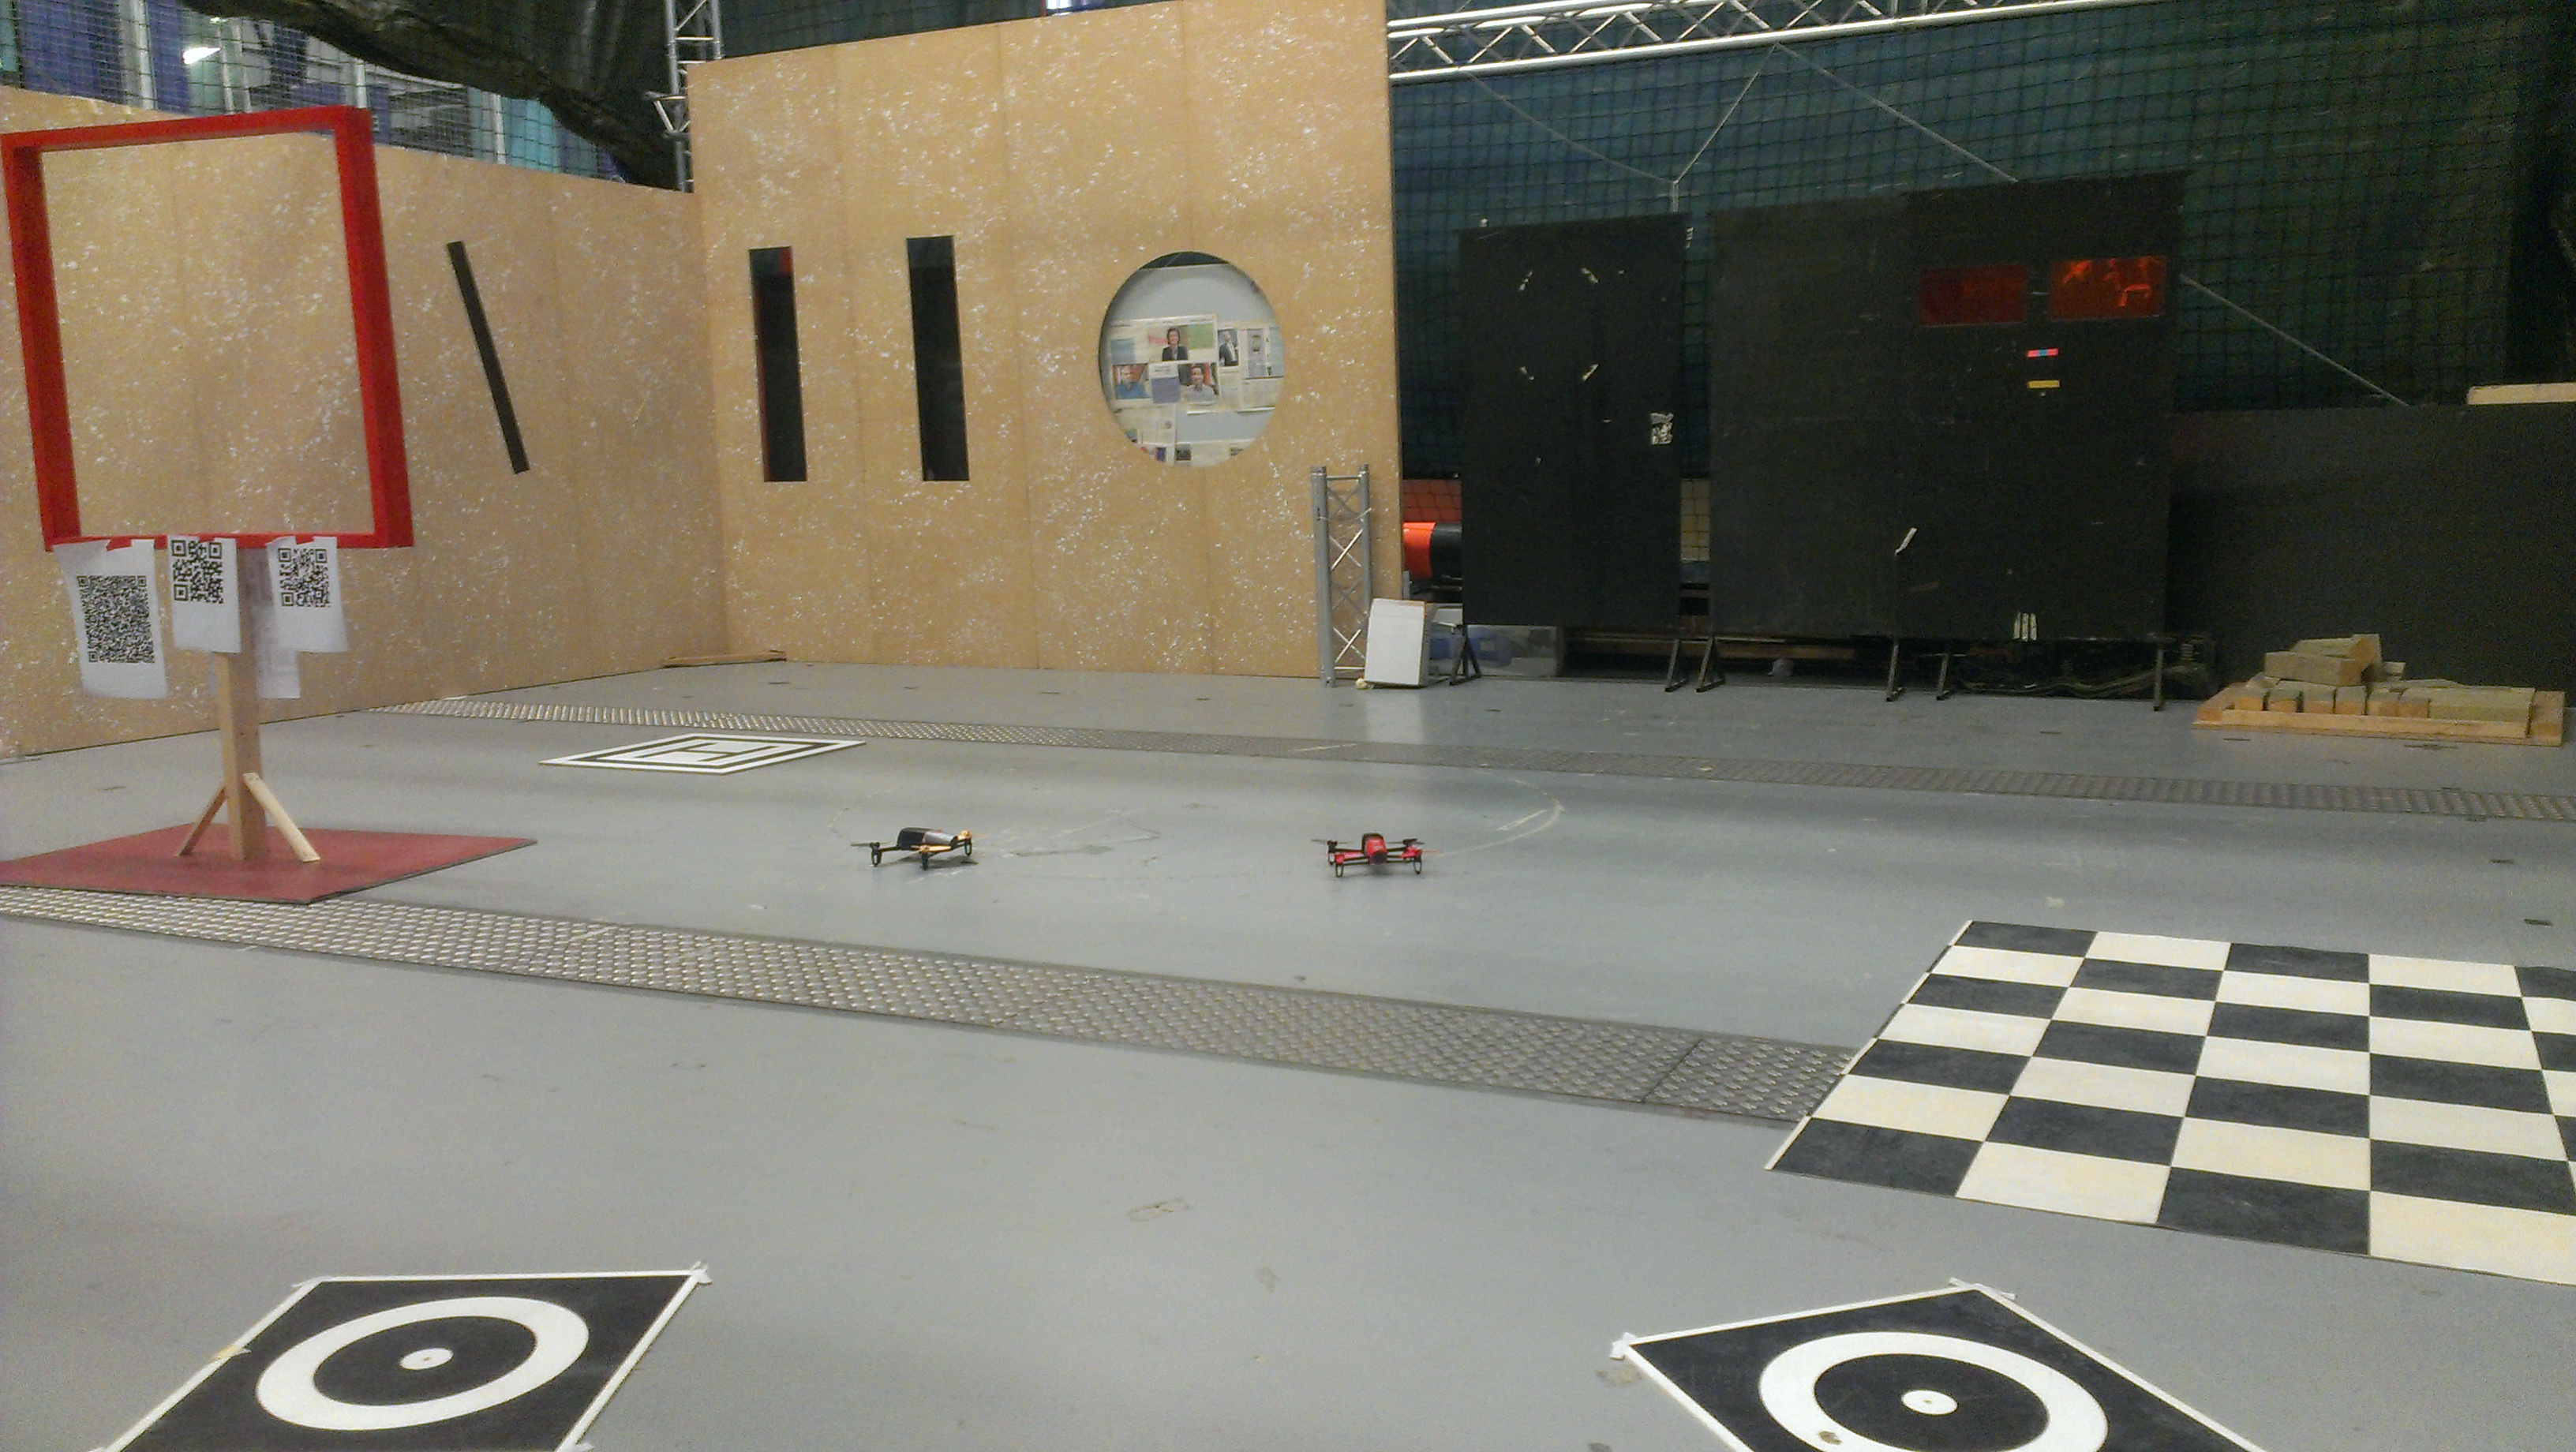
\includegraphics[width=0.8\textwidth]{cyberzoo} 
  \caption{The indoor flight arena at the Delft University of Technology
  }
    \label{fig:cyberzoo}
\end{figure}


%since the proposed algorithm is intended for known
%environments, this is always possible.

\section{Determining the Number of Image Patches}
\label{sec:numtextons}

The computational complexity of the developed framework can be
modified by changing the number of extracted image samples in the
\emph{random sampling} step of the texton histograms creation. Due to
the random sampling of the extracted image patches, the histograms
differ.

Comparing the cosine similarity between the histograms has the
advantage that the number of samples can be estimates independently of
the specific use case.


The goal is to use as few samples as possible, while still obtaining
an adequate localization accuracy.

To determine a suitable number of extracted samples, we compared the
influence of random sampling via the cosine similarity between
histograms in a dataset consisting of $N = 2\,000$ images. The
independent variable is the number of extracted patches $M$ per image.
We used the cosine similarity to obtain similarity values between $0$
and $1$. The similarity was measured at 10, 50, 100, 200, 400, and
1\,000 extracted image patches.

Figure~\ref{fig:cosine} displays the results: the cosine similarity of
histograms as a function of the number of samples and the
corresponding standard deviations.

\unsure{add standard deviation}
\unsure{add accuracy and not only similarity}

\begin{figure}[h!]
\begin{center}
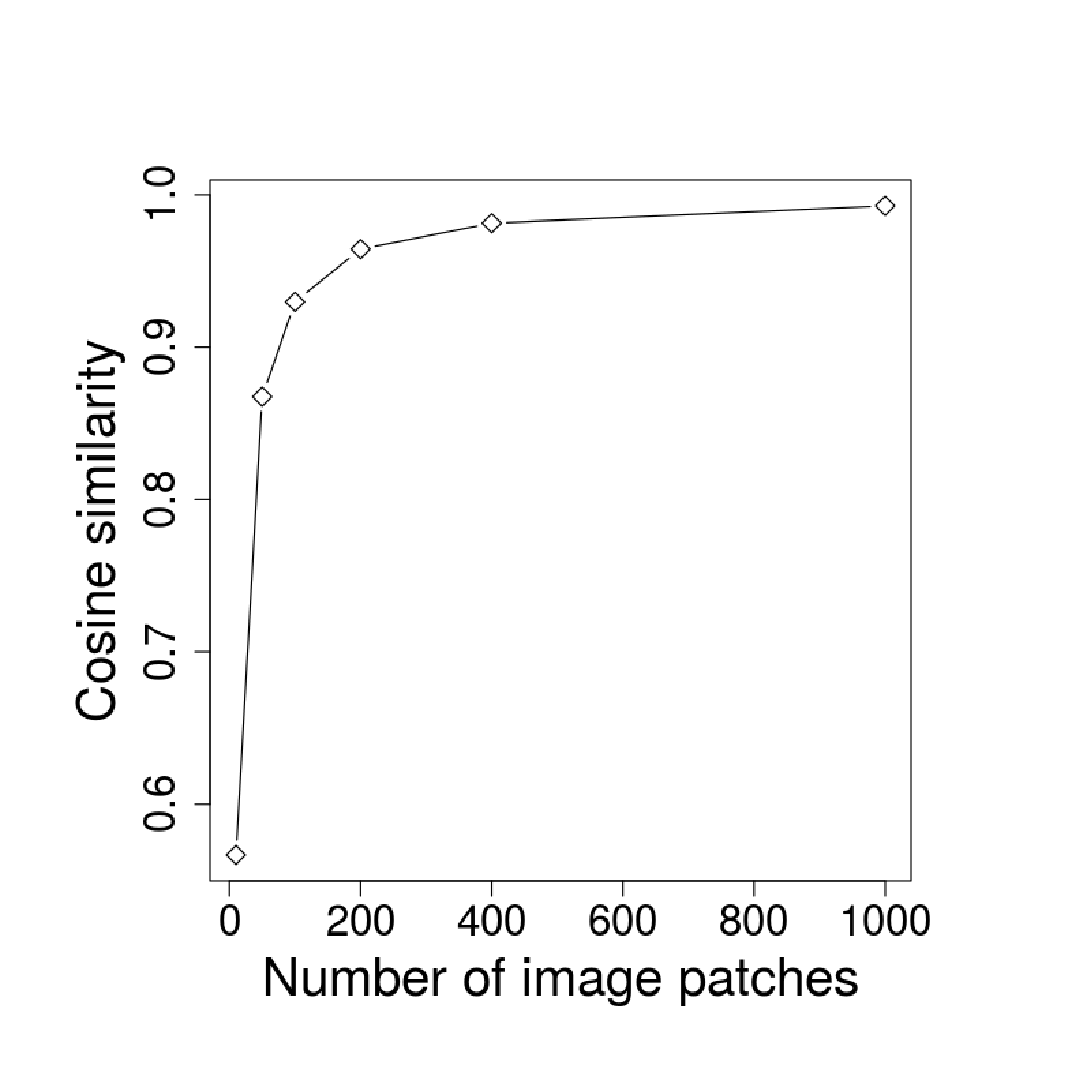
\includegraphics[width=0.5\columnwidth]{samples_vs_similarity}
\caption{{\label{fig:cosine} Cosine similarity of histograms as a
    function of the number of extracted samples \emph{Right}: Standard deviation
    of cosine similarity in relation to the number of samples. The
    squares indicate the positions at which the dependency was
    evaluated.%%
  }}
\end{center}
\end{figure}


\section{Determining $k$ in the $k$-NN algorithm}
\label{sec:detk}

In a standard setting, the training error $\epsilon_t$ of a
$k$=1-nearest neighbor algorithm is $\epsilon_t = 0$ because the
nearest neighbor of the sample will be the sample itself, given that
each feature vector is unique. However, in the presented framework,
the random sampling in the histogram extraction step leads to varying
histograms.


\section{Measurement model for the Particle Filter}
\label{sec:measurementmodel}

As described in Section~\ref{sec:filtering}, we determined the values
$\Sigma^{[j]}$ for the Gaussian mixture measurement model by
calculating the variance-covariance matrix for the difference between
the ground truth $T$ and the predictions $P_j$ of the $k$-NN
algorithm. Figure~\ref{fig:measurementmodel} shows the differences
between these values.

\begin{figure}[h!]
\begin{center}
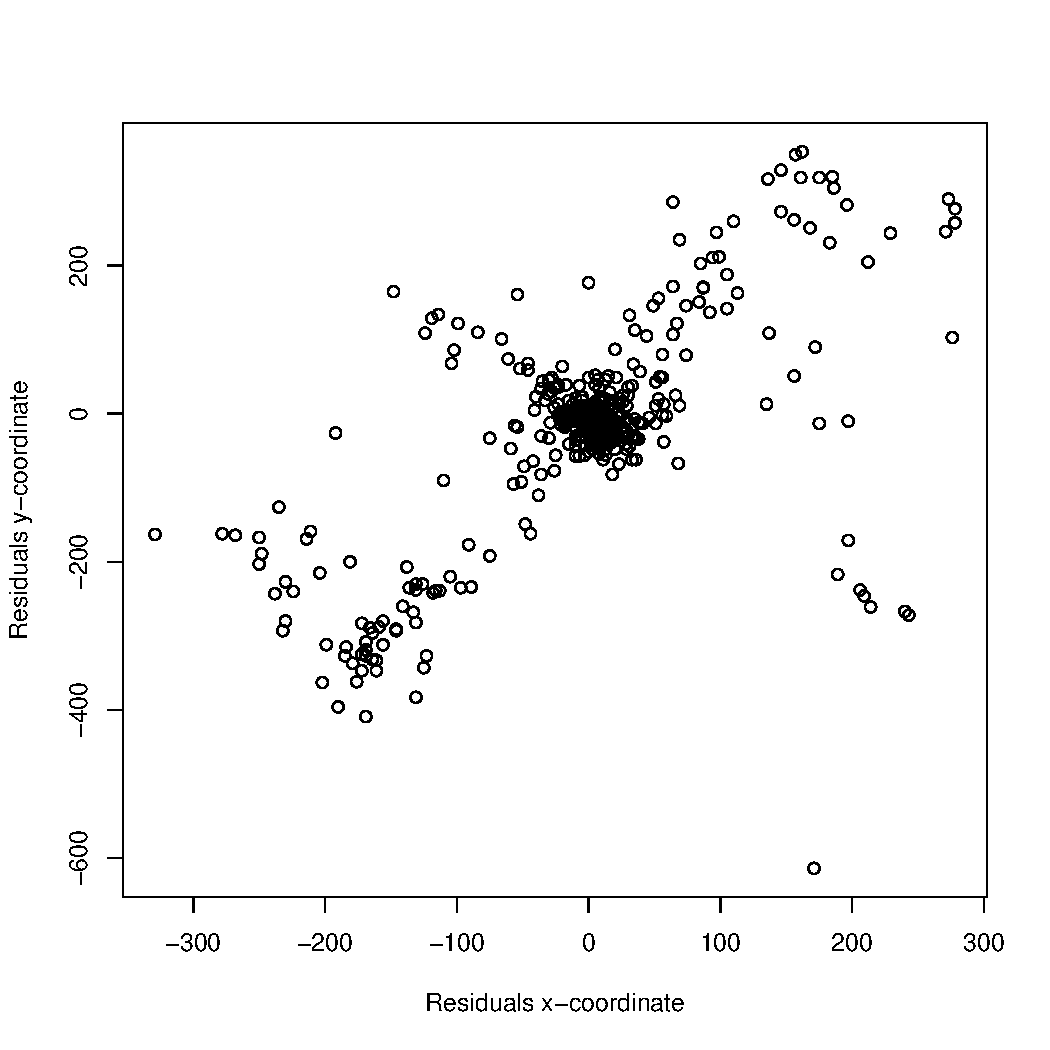
\includegraphics[width=0.7\columnwidth]{measurement_model}
\caption{{\label{fig:measurementmodel}Dependence between error in $x$-direction
    (\emph{Left}) and $y$-direction (\emph{Left}).%
  }}
\end{center}
\end{figure}

\section{Correlation between Histogram Distance and Measurement Error}

As described in Section~\ref{sec:filtering}, we planned to include to
distance to the neighbors in the $k$-NN algorithm as confidence value
for the predictions. Figure~\ref{fig:cor_sim_confi} shows the
correlation between histogram distance and measurement error.

\begin{figure}
  \centering
  \begin{subfigure}[b]{0.5\textwidth}
  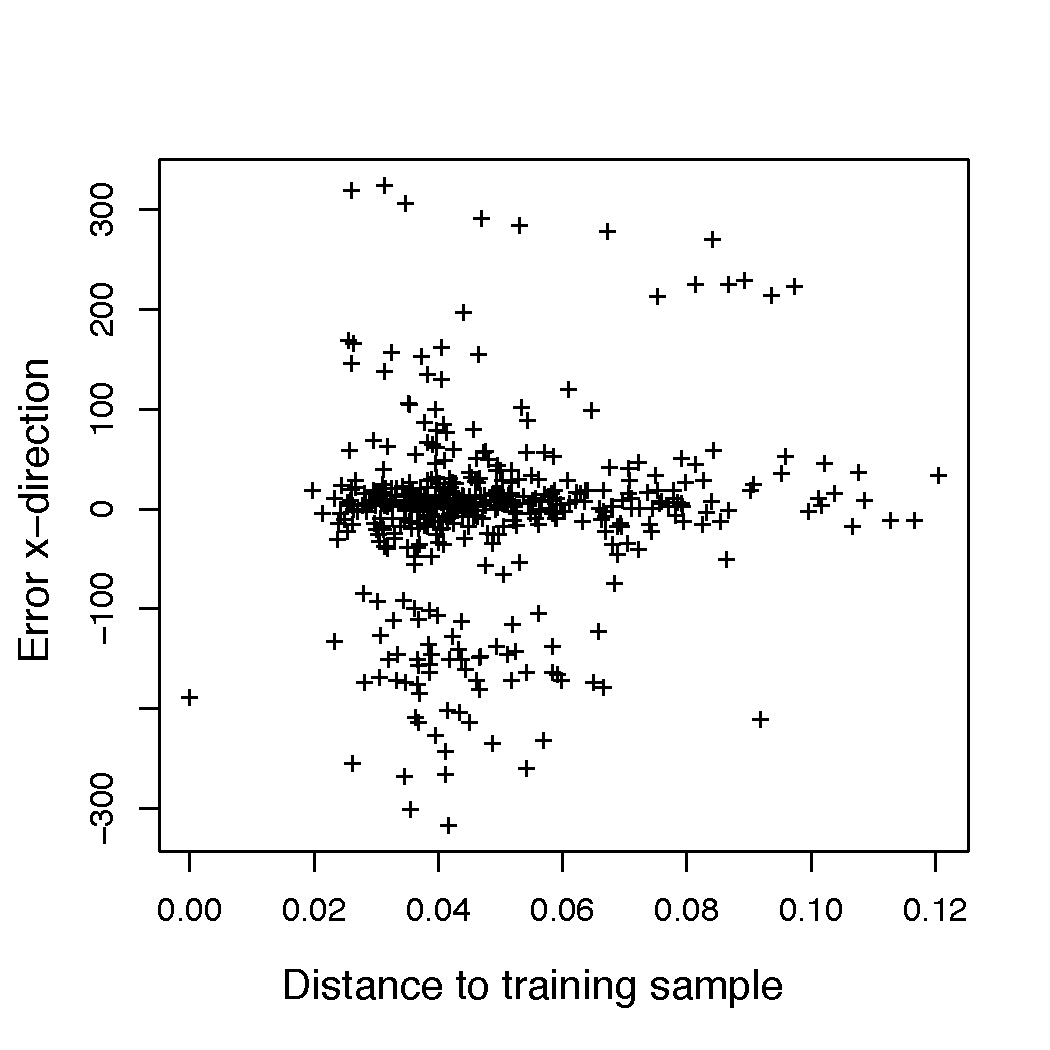
\includegraphics[width=1\textwidth]{dependency_dist_error_x}
    %\captionof{figure}{$POS_x$}
  \label{fig:cosinesim}
  \end{subfigure}%
~
  \begin{subfigure}[b]{0.5\textwidth}
  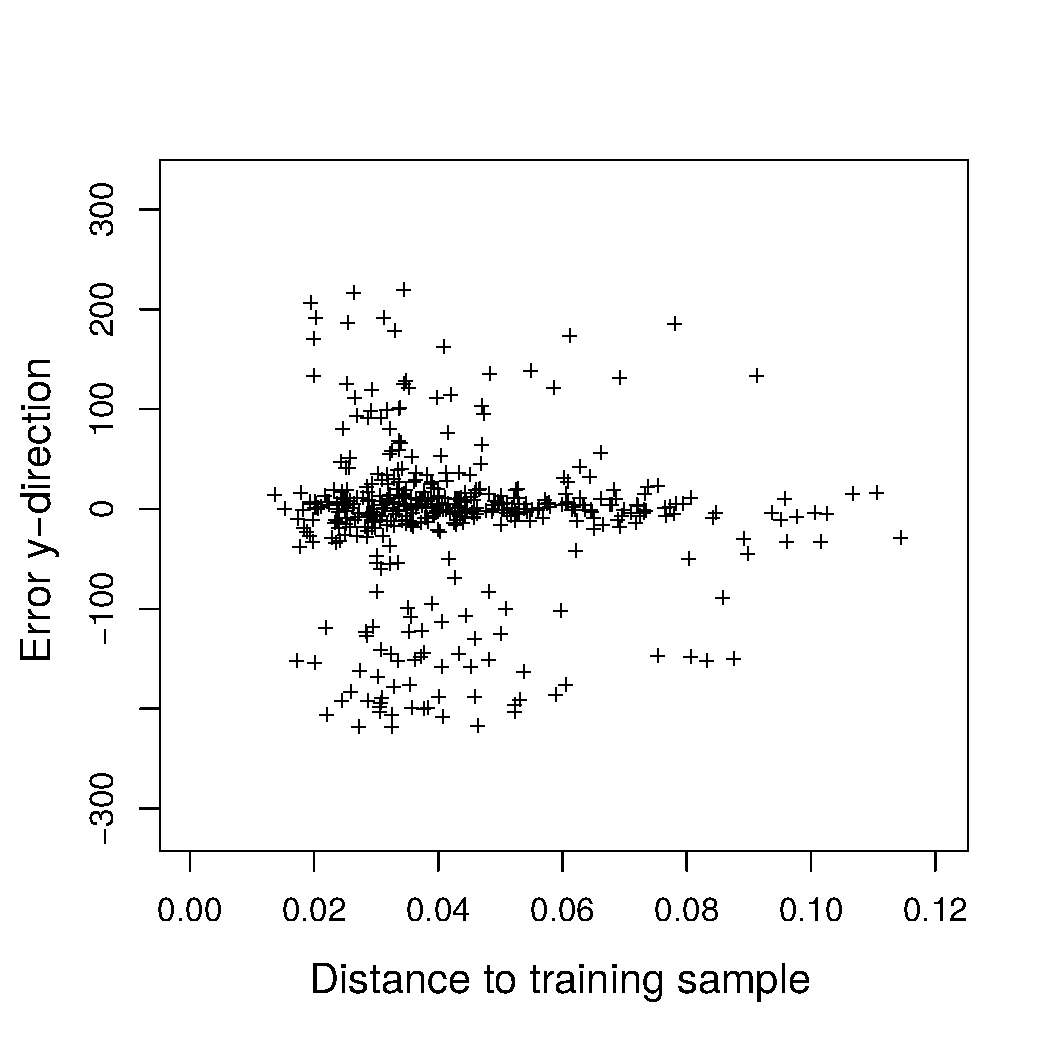
\includegraphics[width=1\textwidth]{dependency_dist_error_y}
   % \captionof{figure}{$POS_y$}
  \label{fig:cosinesd}
  \end{subfigure}
  \caption{Measurement error in $x$-direction (\emph{Left}) and
    $y$-direction (\emph{Right}) as a function of the distance to the
    closest training sample.}
\label{fig:cor_sim_confi}
\end{figure}

\section{Correlation between number of keypoints and Quality of the
  Homography}

Figure~\ref{fig:cosine} shows the correlation between number of
keypoints and the quality of the homography.

\begin{figure}
  \label{fig:cor_keypoints}
  \centering
  \begin{subfigure}[b]{0.5\textwidth}
  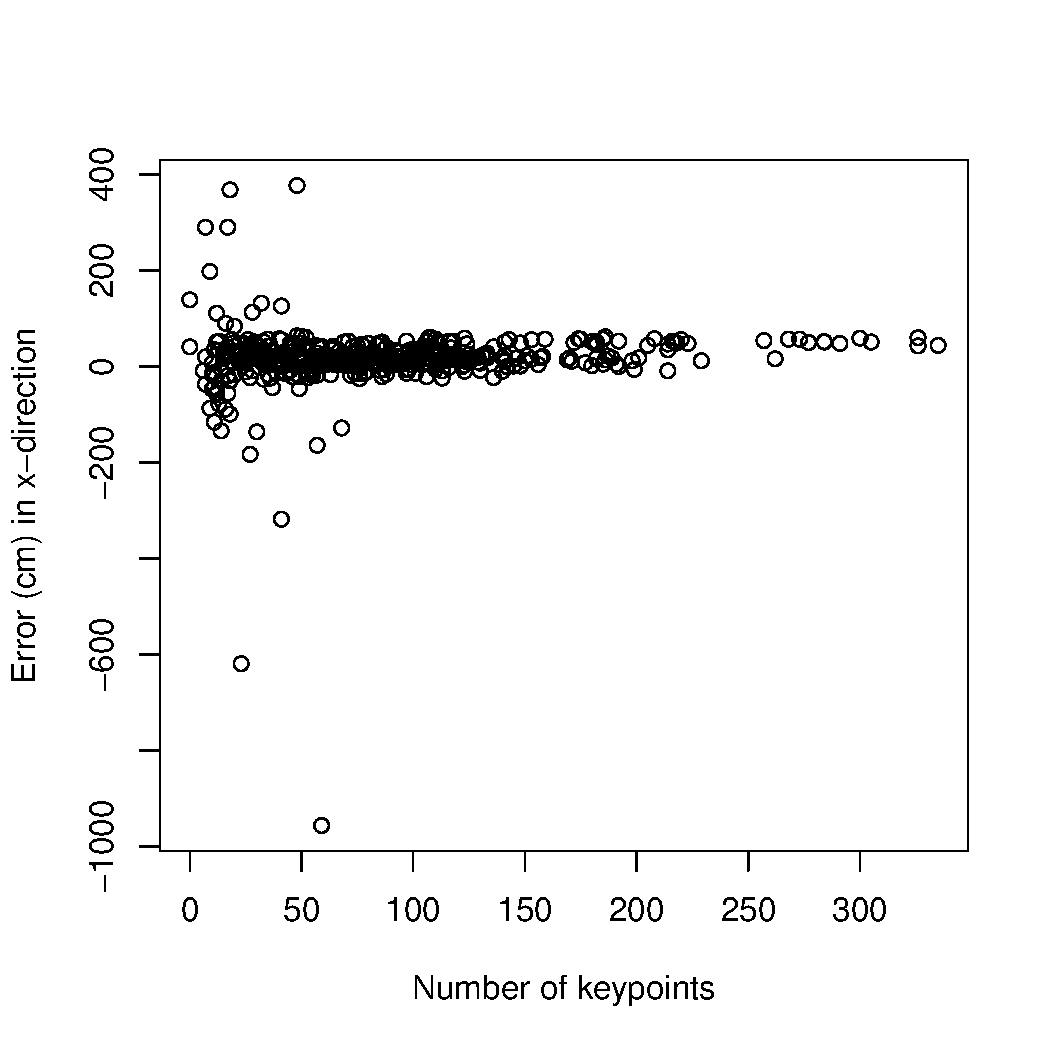
\includegraphics[width=1\textwidth]{keypoints_error_x1}
    %\captionof{figure}{$POS_x$}
  \label{fig:cosinesim}
  \end{subfigure}%
~
  \begin{subfigure}[b]{0.5\textwidth}
  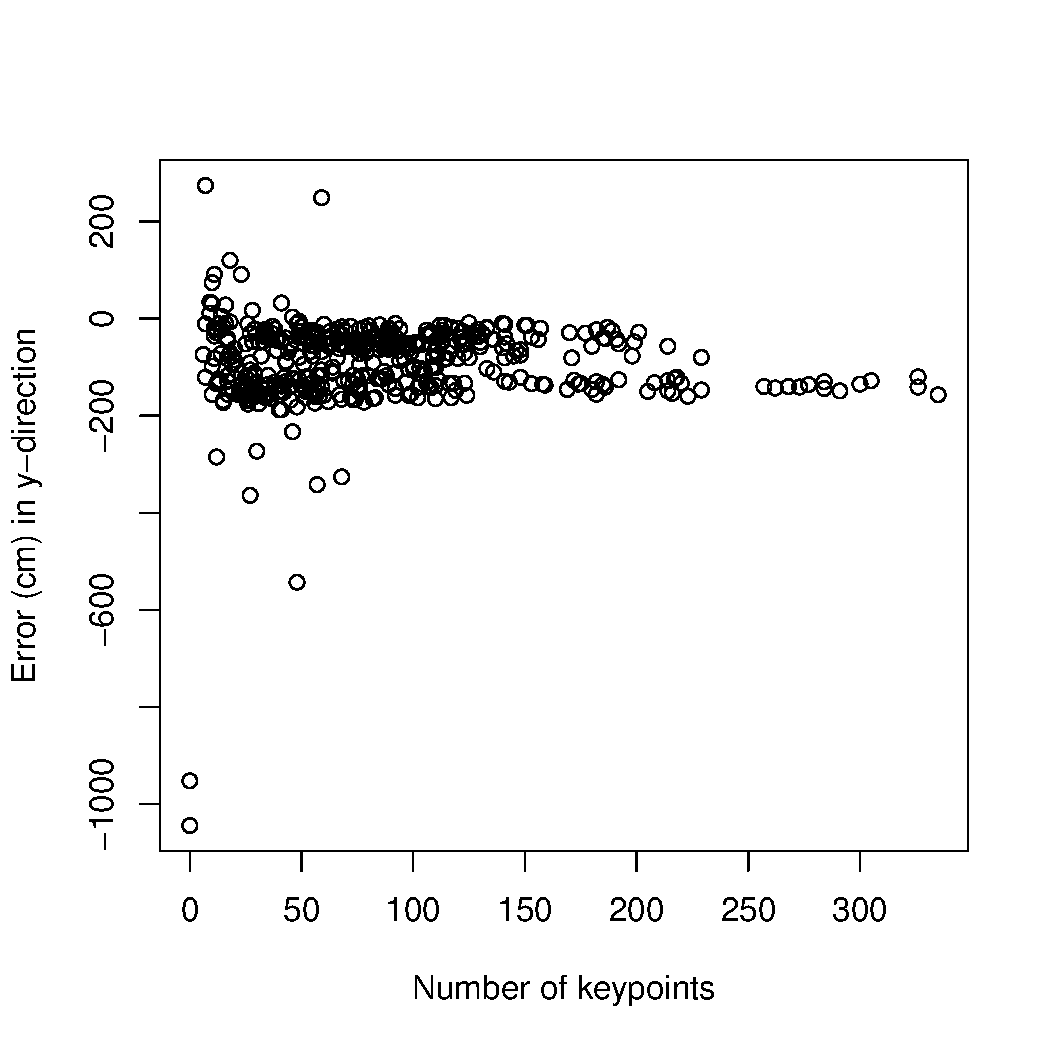
\includegraphics[width=1\textwidth]{keypoints_error_y}
   % \captionof{figure}{$POS_y$}
  \label{fig:cosinesd}
  \end{subfigure}
  \caption{Measurement error in $x$-direction (\emph{Left}) and
    $y$-direction (\emph{Right}) as a function of the number of
    keypoints found by \textsc{Sift}.}
\label{fig:cosine}
\end{figure}

\section{Continuous Coordinate Estimation}

\subsection{Baseline: Compare SIFT and OptiTrack}
\label{sec:siftvsoptitrack}

To find a baseline for our approach, we use the homography-based
approach to estimate $x,y$-coordinates. The required hyperspatial
image (Figure~\ref{fig:mapexp}) of the environment was stitched
together using 500 images and the software Microsoft ICE.

\begin{figure}[h!]
\begin{center}
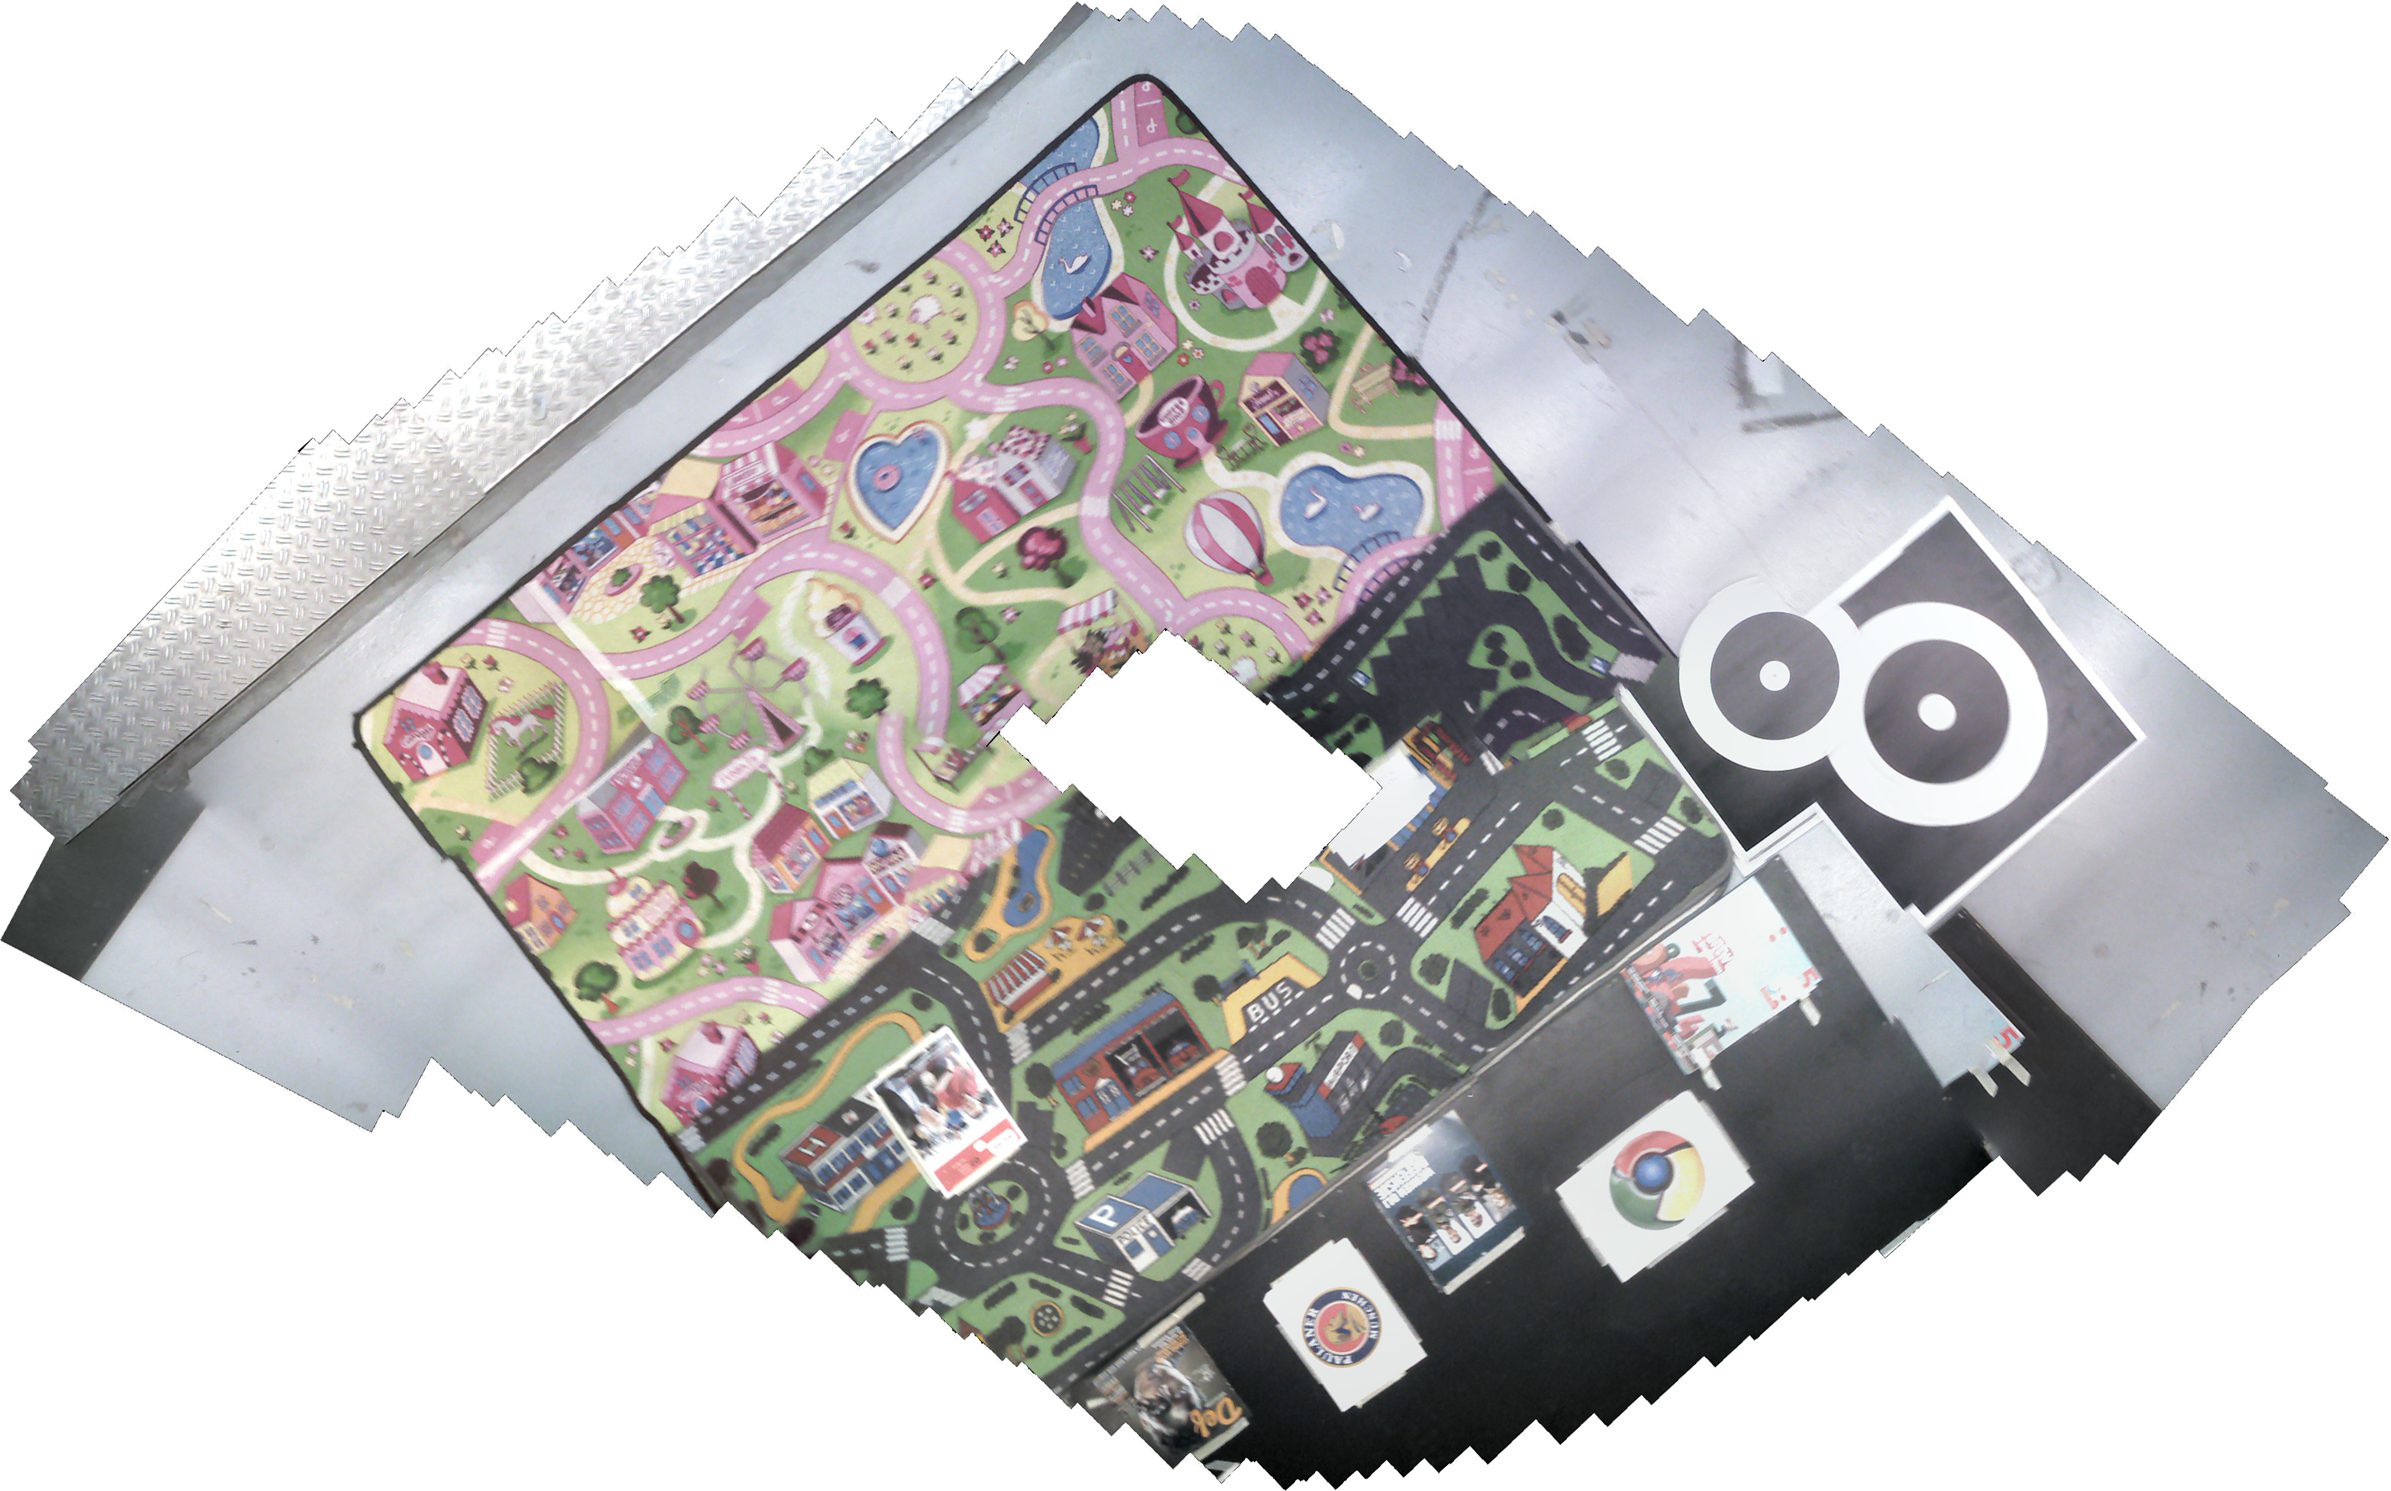
\includegraphics[width=0.7\columnwidth]{map_rotated}
\caption{{\label{fig:mapexp} The created map that was stitched
    together using 445 images. A non-mapped area in the middle of the
    map can be seen, which is a result of the set flight path. An
    image distortion can be seen at the right-hand side, where the
    landing spot sign appears twice, while in reality, only one circle
    was visible.%
  }}
\end{center}
\end{figure}

The results can be found in Figure~\ref{fig:siftestimates} and Table~\ref{tab:homoerror}.

\begin{figure}[h!]
\begin{center}
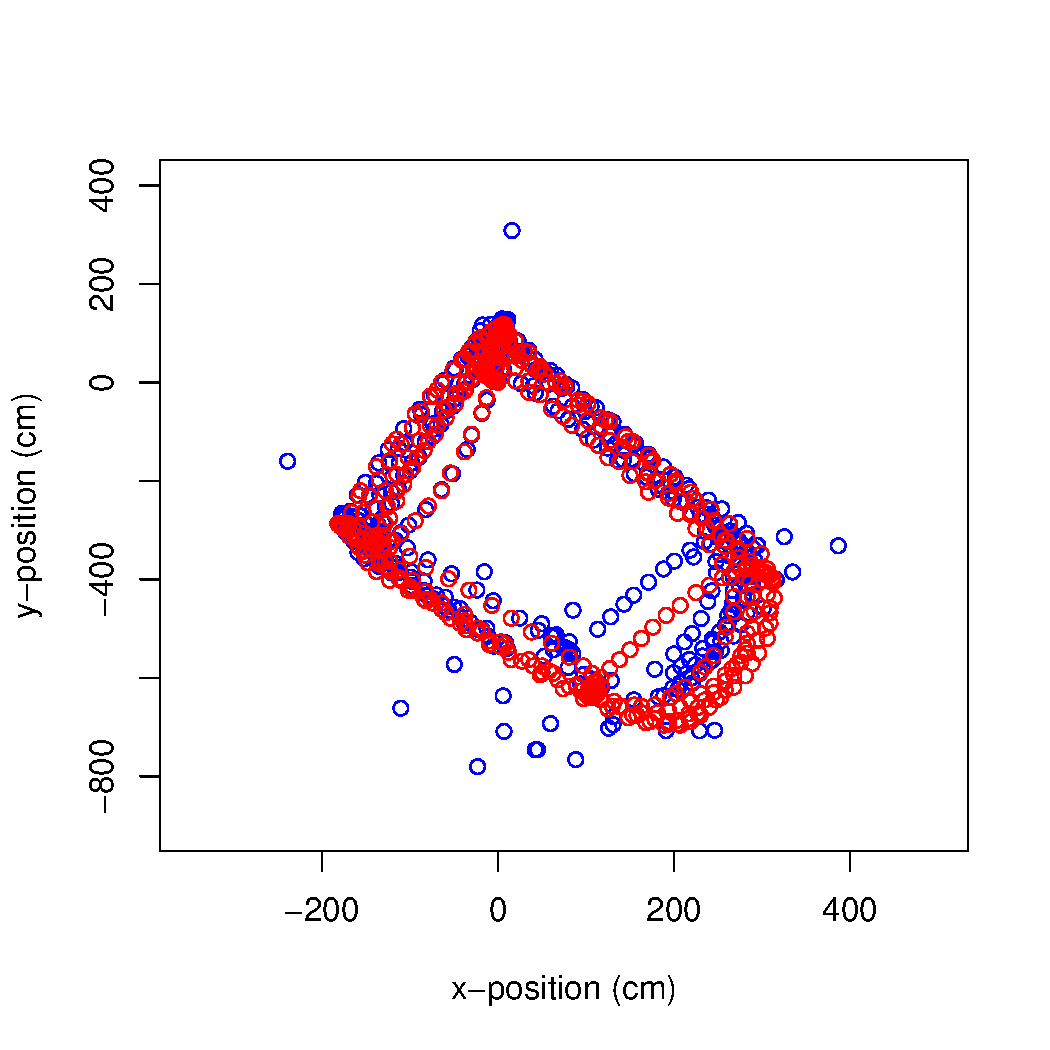
\includegraphics[width=0.7\columnwidth]{SIFT_vs_OptiTrack}
\caption{{\label{fig:siftestimates} The estimates of the homography
    method compared to the ground truth of the motion tracking system.
    TODO: Legend%
  }}
\end{center}
\end{figure}


\begin{table}[H]
  \centering
  \begin{tabular}{lrrr}
    \toprule
    & x-position & y-position\\
    \midrule
    Error in $cm$ & 31 & 75\\
    STD in $cm$ & 73 & 369\\
    \bottomrule
  \end{tabular}
  \caption[Error statistics homography method.]{Error statistics for the homography method.}
  \label{tab:homoerror}
\end{table}


\subsection{Training Set based on Motion Tracking System}
\label{sec:experiment-real}

In this experiment, a fixed flight plan was set in the ground control
station. Stabilization and guidance were performed using the motion
tracking system OptiTrack. The position estimates were calculated on
board of the MAV using the texton-based approach with the particle
filter. The Euclidean distances between the estimates of the motion
tracking system and the texton-based approach were measured in
$x$-direction, $y$-direction and combined as two-dimensional
deviation.

The training dataset was composed of 500 texton histograms with
corresponding $x,y$-coordinates that were obtained from the motion
tracking system. The images were recorded at an height of
approximately one meter in a time span of one hour before the
experiment.

\begin{table}[H]
  \centering
  \begin{tabular}{lrrr}
    \toprule
    & x-position & y-position\\
    \midrule
    Error in $cm$ & 46 & 54\\
    STD in $cm$ & 56 & 71\\
    \bottomrule
  \end{tabular}
  \caption[Estimates of the texton-based approach]{Estimates of the texton-based approach}
  \label{tab:route}
\end{table}

\subsection{Training Set based on Homography-finding Method}
\label{sec:traininghomo}

In this experiment, the training dataset was created using the
homography-finding method. Apart from that, the settings are the same
as in Experiment~\ref{sec:experiment-real}.

The estimates of the homography-based approach compared to the motion
tracking system OptiTrack can be found in Figure~\ref{fig:flightpath}. 

\section{Experiment -- Triggered Landing}
\label{sec:triggered}

For the triggered experiment, the MAV was instructed to fly along a
set of random flight paths, which covered the $5 \times 5$ meters
area; during the navigation, the MAV was programmed to land as soon as
its position estimates were in a ``landing zone'': a $x,y$-position
with a specified radius $r$. A safety criterion based on the variance
of particles was introduced, such that the landing is only performed
if the criterion holds. The criterion parameter was set to 60\,cm in
both $x-$ and $y$-direction.

For the texton framework, the same training set as in
Experiment~\ref{sec:experiment-real} was used. The $x,y$-coordinates
of circle was specified in the flight plan; the radius was set to $r =
60\,cm$. We performed six triggered landings; after each landing, the
$x-y$-center of the zone was randomly set another position in the map.


%The experiment was conducted on an approximately $5m \times 5m$ map
%and the ground truth was based on the position data from the motion
%tracking system.

%Table~\ref{tab:targetlanding} shows the results of the triggered
% landings.

Four out of six landings were correctly performed in the landing
area. The mean distance of the two outliers was 16\,cm measured as
distance to the circumference of the landing area.
%\begin{table}[H]
%  \centering
%  \begin{tabular}{lrrr}
%    \toprule
%    & x-position & y-position\\
%    \midrule
%    Error in $cm$ & TODO & TODO\\
%    STD in $cm$ & TODO & TODO\\
%    \bottomrule
%  \end{tabular}
%  \caption[Triggered landings]{Results of the triggered landings}
%  \label{tab:targetlanding}%
%
%\end{table}

\section{Experiment -- Determining the Frequency}

The frequency of the proposed algorithm is determined by varying the
following parameters:
\begin{itemize}
\item number of samples in the texton-based approach
%\item number of textons
\item number of particles of the particle filter.
\item number of histograms in the training set
\end{itemize}

While there are further tune-able parameters, they did not have a
large influence on the run-time and were, therefore, not analyzed in
detail.
%Their contribution to the run-time can be neglected.

\begin{figure}[h]
  \centering
  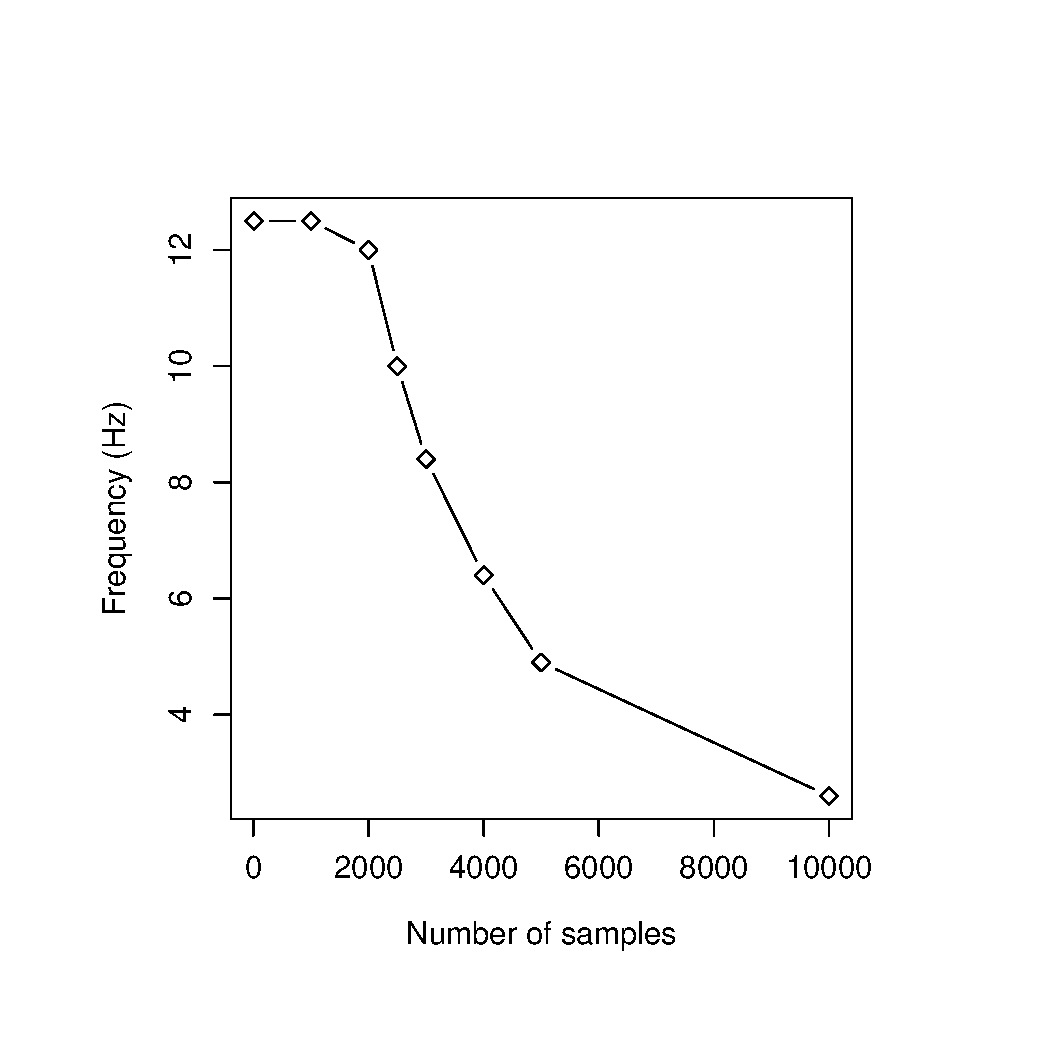
\includegraphics[width=0.7\textwidth]{samples_vs_freq}
  \caption{Frequency of the main loop as a function of the number of extracted samples.}
  \label{fig:freqsam}
\end{figure}

\begin{figure}[h]
  \centering
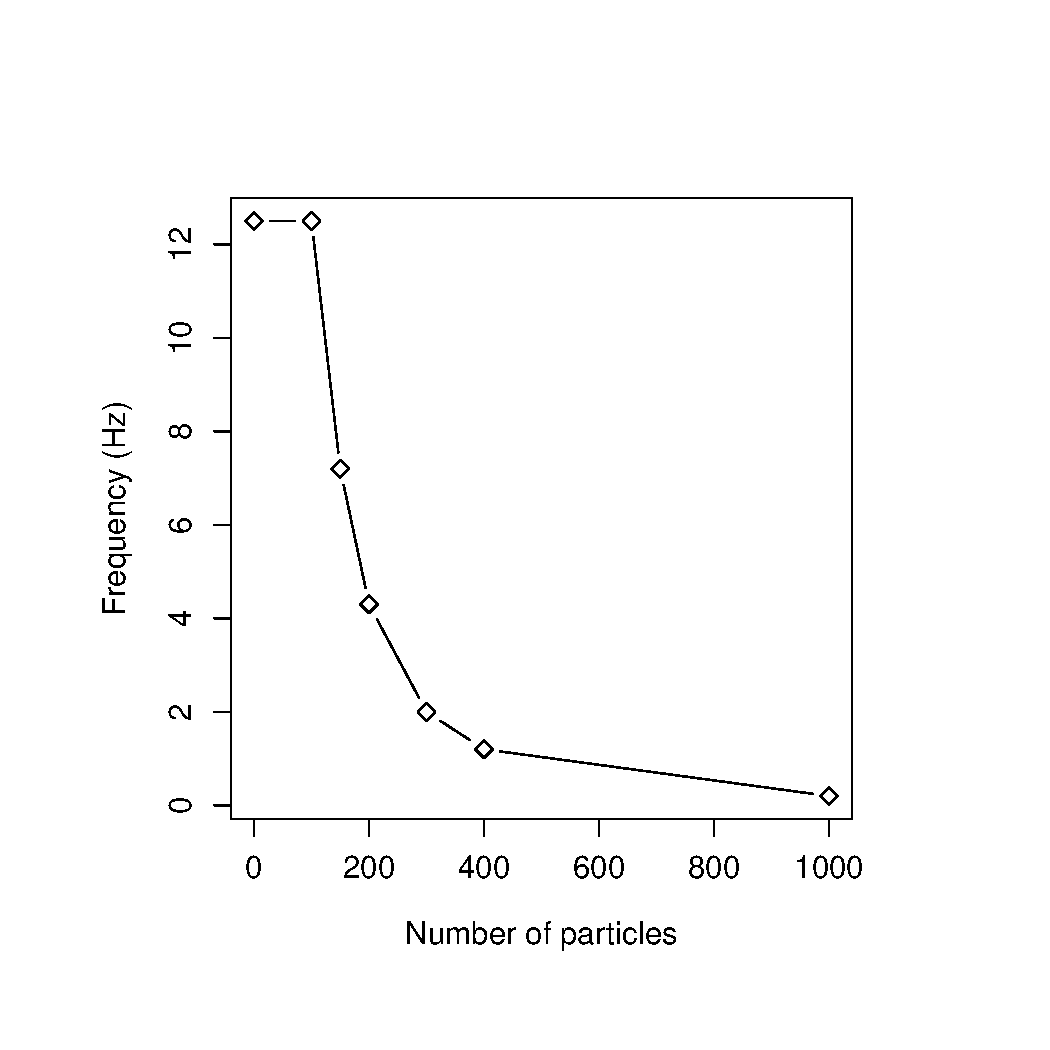
\includegraphics[width=0.7\textwidth]{particles_vs_freq}
  \caption{Frequency of the main loop as a function of the number of
    particles in the particle filter.}
  \label{fig:freqpart}
\end{figure}

\begin{figure}[h]
  \centering
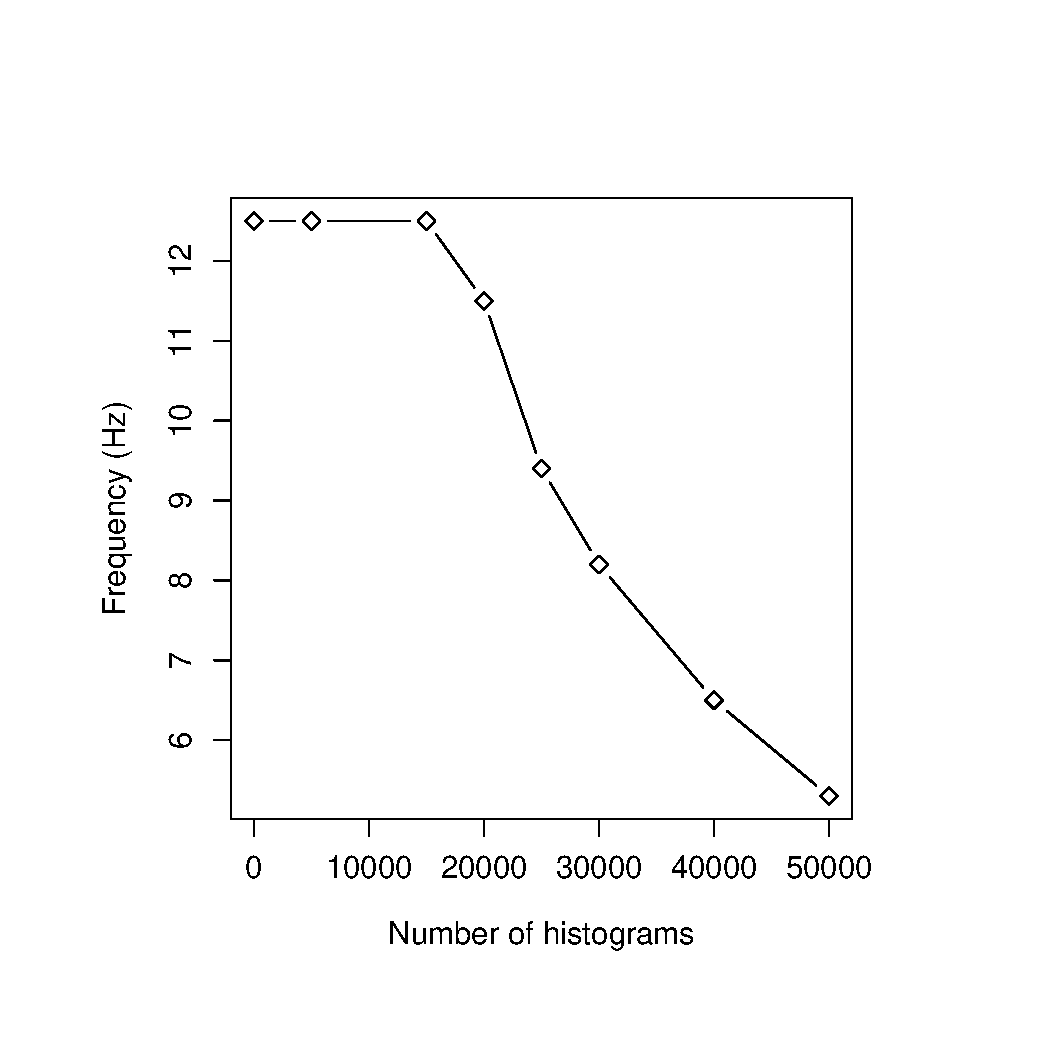
\includegraphics[width=0.7\textwidth]{histograms_vs_freq}
  \caption{Frequency of the main loop as a function of the number of
    histograms in the training set.}
  \label{fig:freqpart}
\end{figure}


\section{Experiment -- Comparing different possible maps}

For the map comparison, 46 possible maps have been collected using the
search term `wallpaper' in Google's image search. This search term was
used, since it is (i) a general term, without any specific image
categories, (ii) wallpapers are likely to have a high resolution, and
(iii) wallpapers are often visually pleasant. Only images with a
minimum resolution of $1\,920 \times 1\,080$ pixels were
chosen. Images with a higher resolution were converted to
$1\,920 \times 1\,080$ pixels. For each image, we generated $1\,000$
random image patches using the synthetic data generation tool
described in Section~\ref{sec:syntheticdatageneration}, followed by
the histogram extraction. This yielded a labeled dataset of histograms
and corresponding positions. For each map, we determined the expected
overall loss based on the method described in
Section~\ref{sec:syntheticdatageneration}. The compared maps were then
sorted according to their estimated loss.

%Three of the compared maps---the
%best performing, the one with median performance, and the worst
%performing---were printed on A0 paper to test the performance in the
%real world.


In Table~\ref{tab:mapeval}, the results of the map evaluation
procedure for the $N = 46$ maps are shown.

\begin{table}[h]
  \centering
  \begin{tabular}{lr}
    \toprule
    Statistic & Value\\
    \midrule
    mean & 0.57\\
    median & 0.55\\
    standard deviation & 0.14\\
    max & 0.99\\
    min & 0.24\\    
    \bottomrule
  \end{tabular}
  \caption[Map evaluation procedure on synthetic data]{Results of the map evaluation procedure on synthetic data}
  \label{tab:mapeval}

\end{table}

Figure~\ref{fig:minmaximg} shows the map with the highest global loss
value and the map with the lowest global loss value.

\begin{figure}[h!]
\begin{center}
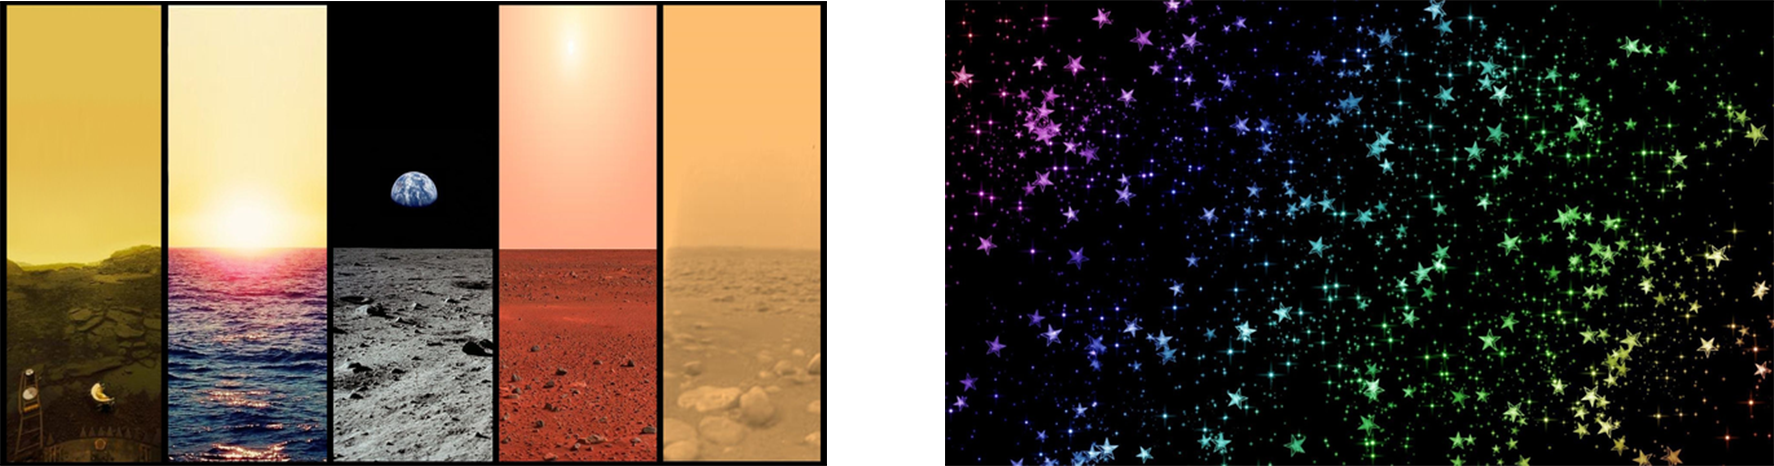
\includegraphics[width=0.7\columnwidth]{lowest_highest}
\caption{{\label{fig:minmaximg}
Image with the lowest loss value; \emph{Right}:
    Image with the highest loss value%
}}
\end{center}
\end{figure}

\chapter{Discussion}
\label{chap:discussion}

In this chapter, the results of the experiments are discussed with
regards to accuracy, frequency, and future improvements. Afterward, in
the General Discussion, the research questions are addressed and
discussed.

The comparison between sub-sampling and full sampling
(Experiment~\ref{sec:numtextons}) has shown that only a small part of
the maximum amount of samples is necessary. In fact,
$\frac{400}{640 \times 480} = 0.13\,\%$ of the maximum amount of
samples suffices to achieve cosine similarities between the texton
histograms larger than $99\,\%$. This set the stage for large
speed-ups during live operation. Additionally, the technique allows
for further speed-ups depending on the processing power of the
platform at hand.

In the real-time position estimation experiment
(Experiment~\ref{sec:experiment-real}), the initial mean error
was rather large: 130\,cm in $x$-direction and 90\,cm in
$y$-direction. A more in-depth analysis revealed that the estimates of
the particle filter were lacking behind the position estimates of the
motion tracking system. This was due to the simple motion model of the
particle filter that was based on Gaussian noise only. By shifting the
estimates of the particle filter by six frames, that is approx. 0.46
seconds at a frequency of 13\,Hz, the error could be reduced to 46\,cm
in $x$-direction and 54\,cm in $y$-direction. This lag can be
addressed by to strategies: (i) slower speed during flight, (ii) a
better or more flexible motion model.

The triggered landing (Experiment~\ref{sec:triggered}) showed a high
accuracy. While most landings were triggered inside the landing zone,
two out of the six landings were outliers. However, their distance to
the landing area were rather small, with an average distance of
16\,cm. A comparison without the safety criterion, showed, that the
criterion can have advantages.

The evaluation of different maps using the synthetic data showed high
differences between the evaluated images. The range of losses from
0.24 to 0.99 underlines the varying suitability of different maps for
the proposed algorithm.
% To visually evaluate the map evaluation technique, a simple map was
% constructed with two repeating tiles.
The
image with the minimum and the one with the maximum loss value based
on their color histogram are shown in Figure~\ref{fig:minmaximg}. The
different patterns of the images are clearly visible: while the image
with the minimum value fulfills the desired properties---closeby areas
have similar color values, distant areas are dissimilar, the image
with the maximum loss is mainly black resulting in similar histograms
all over the place and leading to high loss values. This initial
evidence can be taken to test the predictive power of the evaluation
algorithm for texton histograms.

There are no generally optimal parameters for the presented framework:
Setting the number of textons, the number of images patches, or the
number of neighbors is dependent on the environment and the size of
the training dataset. The parameters have to be adapted to the
particular environment.

\section{General Discussion}
\label{sec:generaldiscussion}

In this thesis, we addressed the problem of estimating
$x,y$-coordinates in real-time and on-board of an MAV. We identified a
computer vision-based approach the be most suitable due to the limited
payload capacity of MAVs. We recapitulate the research questions
(RQs):

\begin{itemize}
\item \textbf{RQ\,1:} ``\emph{Can 2D positions be estimated in real-time using a
    machine learning approach on a limited processor in a modifiable
    indoor environment?}''
\item \textbf{RQ\,2:} \emph{``How can we predict and evaluate the suitability of a
    given map for the developed localization approach?''} 
\end{itemize}

Regarding RQ\,1, the conducted experiments provide supportive evidence
that a texton-based machine learning approach is able to accomplish
real-time indoor localization. The proposed algorithm runs with a
frequency of 15\,Hz on a single board computer with limited
CPU. Shifting processing power to an offline training step by creating
a training set and relying on random sampling are the cornerstones of
the developed algorithm.


%Despite the small ratio between extracted
%image patches ($s$) and the maximum amount of different image matches
%($s*$), the accuracy is hardly affected, and only slightly improves
%when incorporating more textons.

We still need to find evidence that the proposed map evaluation
generalizes to the real-world. In contrast to R\,1, the generalization
from the synthetic data to real-world data is of a different nature in
this case. The requirement here is that maps that follow the ideal
similarity distribution in the synthetically generated images also
follow this distribution after being recorded with a camera. Or stated
differently, for maps with a low loss value, distant image positions
should not have similar histograms using the synthetic images nor the
real-world images. Which is an easier problem.

Despite the overall promising results, we noticed drawbacks of the
developed approach during the flight tests and identified several
directions for future research that are described in what follows. The
developed method sets the stage for numerous future research
directions and improvements.

The accuracy---that is the difference between the estimates of the
motion tracking system and the texton-based approach--- could be
further improved by incorporating more features, for example histogram
of oriented gradients.
%Additional improvements could be obtained by
%investigating further regression techniques, like Gaussian processes
%or Bayesian networks that can inherently handle space and time.

% Write about general rotations
The current implementation assumes rather constant height up to few
centimeters and no rotations of the MAV. While a quadroter can move in
every direction without performing yaw movements, other MAVs or the
use of the front camera for obstacle avoidance could require yaw
movements. The inclusions of images into the dataset of arbitrary yaw
movements would possibly inflate the size of the dataset to a too
great extent. This could lead to a deterioration of the accuracy and
highly increase the time-complexity of the $k$-NN algorithm. Instead,
a ``derotation'' of the camera image could be performed to align it
with the underlying images of the dataset. We developed a prototype
for procedure (Figure~\ref{fig:rotation}). The rotation is done on the
basis of data from the inertial measurement unit (IMU), which is a
sensor that measures the angular displacement of the MAV. An initial
version of such a system can be found in out GitHub
repository\footnote{\url{https://github.com/Pold87/derotator}}.

\begin{figure}[h]
  \centering
  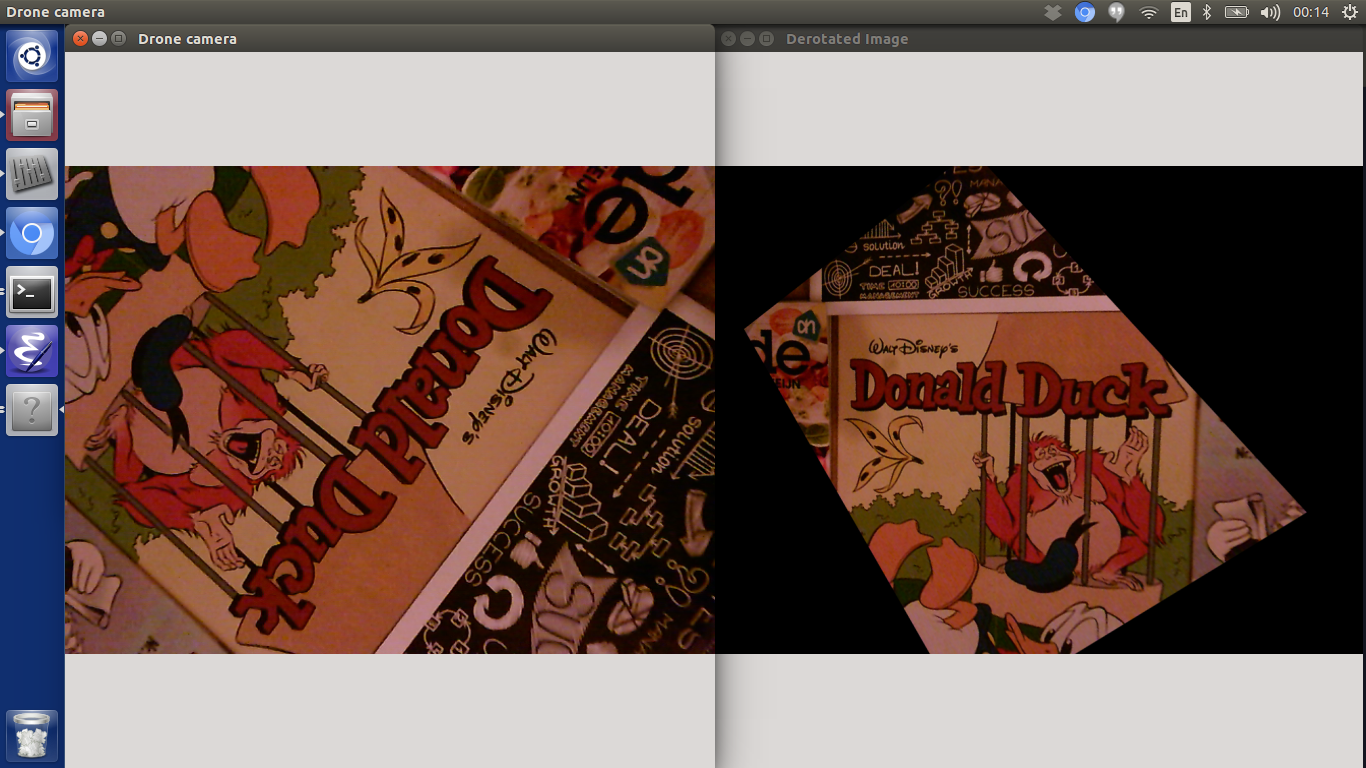
\includegraphics[width=0.8\textwidth]{derotator}
  \caption{The perspective transformation which is due to the rotated
    camera has been removed by applying a reverse transformation.}
  \label{fig:rotation}
\end{figure}

While the current map evaluation approach used existing fixed images,
it could also serve as a fitness function for an optimization
approach---for example, an evolutionary algorithm---which modifies a
given image. This could find a near optimal solution for a given
regression technique and give insightful view in the underlying
structure of certain regression techniques. While the solution to a
loss value of zero or near zero might be unique and independent of the
original image, a higher loss value might change the initial image
only to a certain extent, yielding an ``improved version of the
image'', which is better suited for the proposed algorithm and still
visually pleasant.


Our initial idea to use the synthetic images
(Section~\ref{sec:syntheticdatageneration}) directly as training
data was not successful and not further followed up.
%This might be
%also the reason that only few projects have used synthetic images for
%real-world phenomena.
The reality gap between the synthetic data and real-world data was too
large: Figure~\ref{fig:realitygap} shows an example of two image
patches, one synthetically generated, one taken with the camera of the
MAV. While the patches can be easily identified as similar for human
eyes, the texton maps, where different colors represent different
textons, are dissimilar. Blur, lighting settings, and camera
intrinsics modify low-level features of the image to a strong extent.
The texton images in the figure show that corresponding regions get
classified into different textons, resulting in different
histograms. This makes the transfer from the synthetic data to the
real world difficult.
A possible improvement might be to find a mapping from histograms of
synthetic images to histograms of real images, by mapping ``synthetic
textons'' to ``real-world textons.''

The presented synthetic data generation software generates image
patches based on drawing samples from parametric distributions
only. This was motivated by the fact that an ideal map should be
independent of previous estimates and based on single images
only---ideally requiring no filtering to address the kidnapped robot
problem. In the future, the synthetic flights could be performed by
simulating a continuous route above the image. This would allow to
test the ability of the particle filter on synthetic flights.

\begin{figure}[h!]
\begin{center}
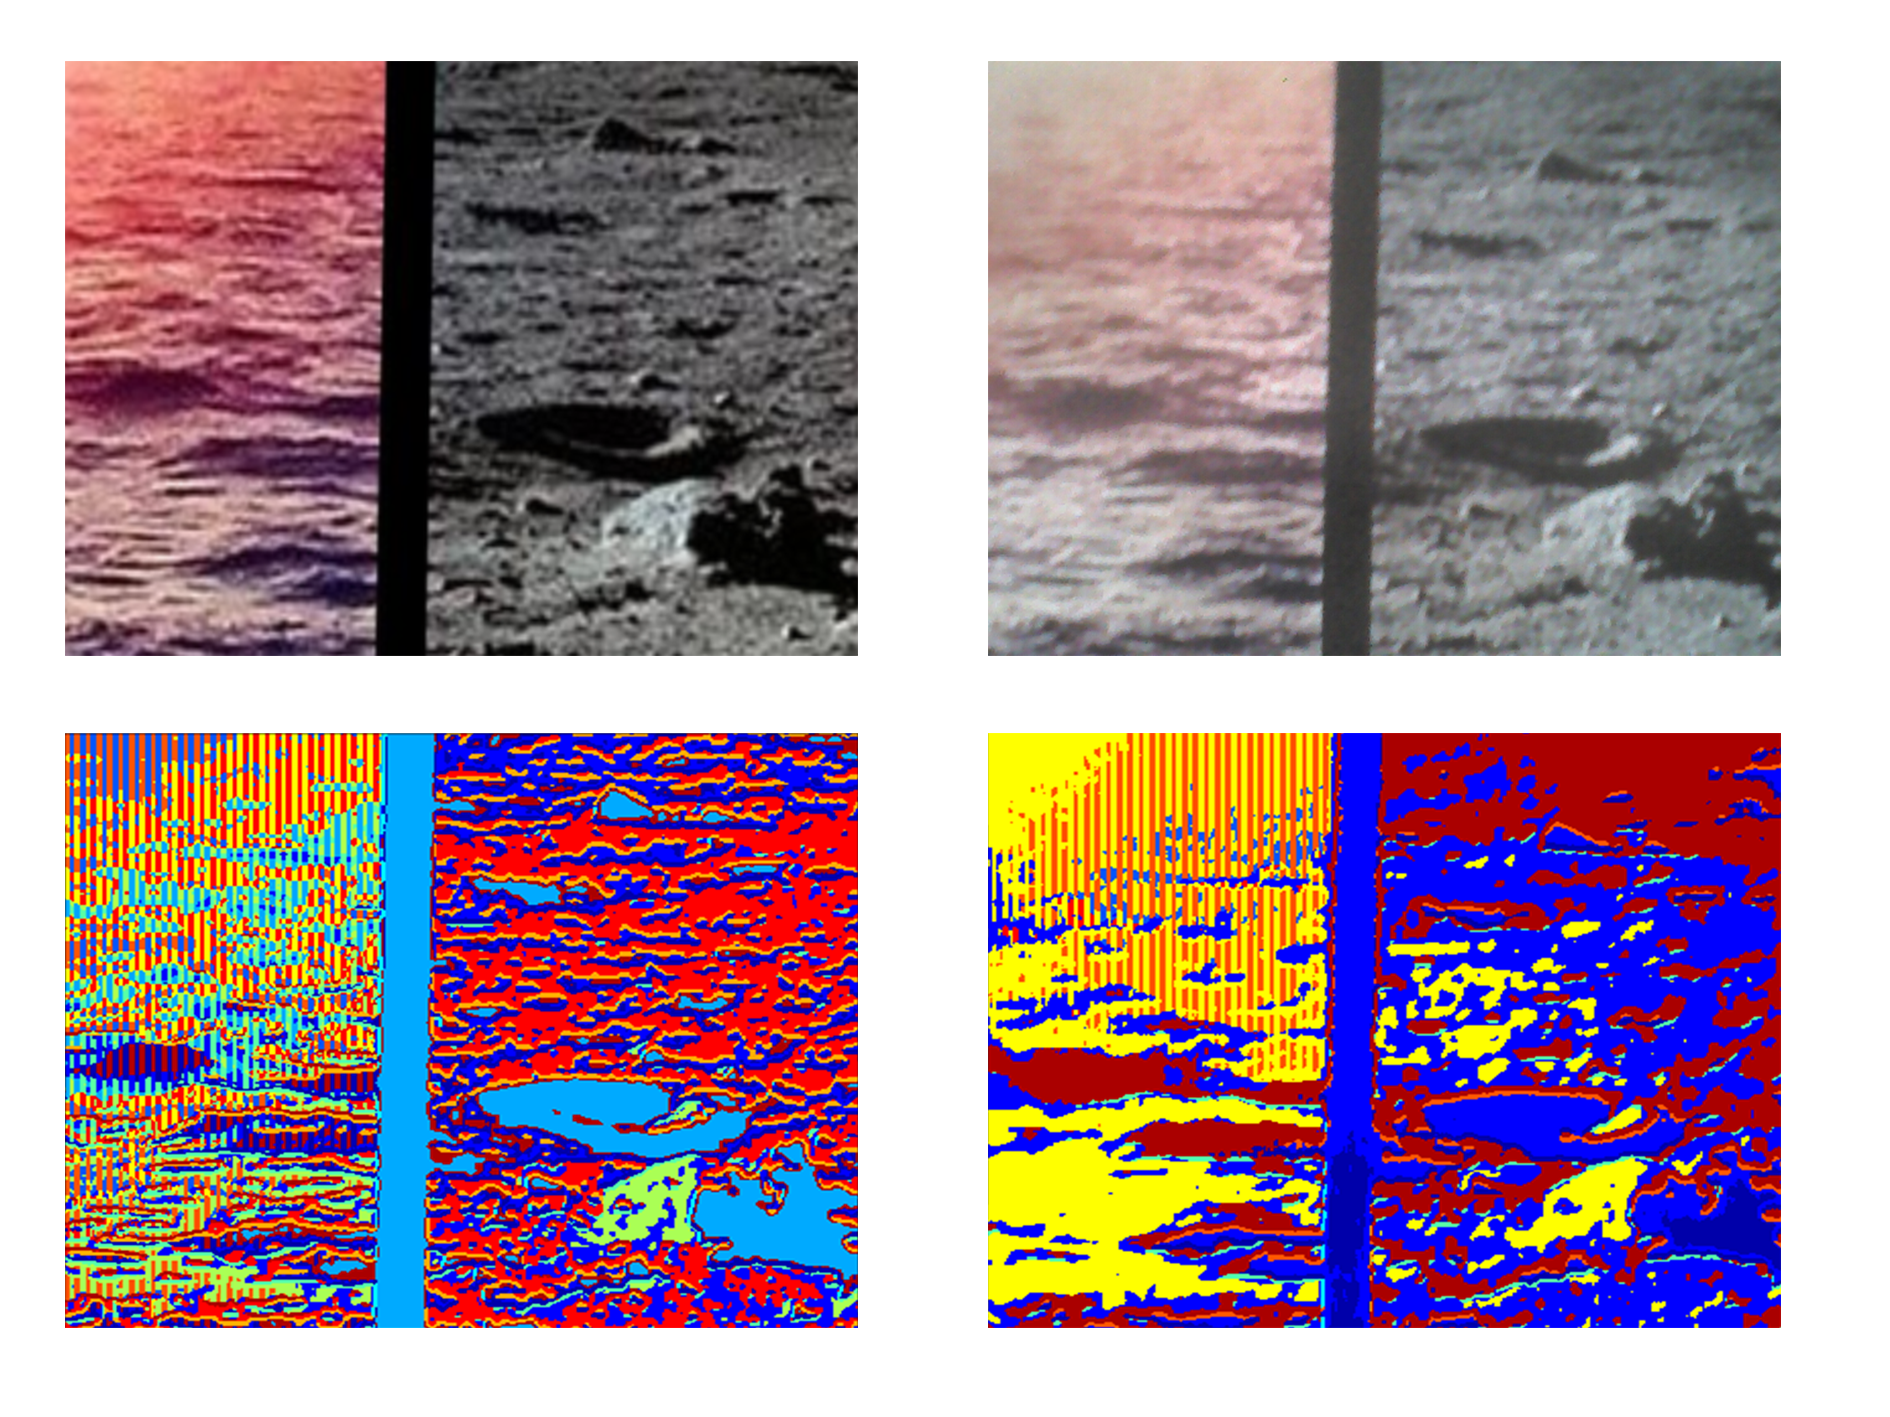
\includegraphics[width=0.65\columnwidth]{realitygap}
\caption{{\label{fig:realitygap} Exemplifying the reality
    gap. \emph{Top left}: image patch generated using the synthetic
    data generation tool. \emph{Top right}: image patch taken with the
    MAV's camera after printing the patch. \emph{Below left}: Texton
    image of the synthetic image. In the image, the colors indicate
    the closest texton (dictionary size: 20 textons) at the respective
    position. \emph{Below right}: Texton image of the real image.  }}
\end{center}
\end{figure}

The shift of the processing power could be further amplified by using
a different regression technique. In the current implementation using
$k$-NN regression, larger training data sets are penalized due to a
greater prediction time. The $k$-NN algorithm should be best
performance in our test. However, the choice of a different regression
technique is not as straightforward as it might seem. The technique
should be able to output multiple predictions, since certain map
regions might be ambiguous.

The presented approach is a vision-only approach. This makes it robust
to external disruptions such as magnetic fields and reduces the amount
of points of failure. Additionally, the approach can be used on
different devices, such as handheld cameras. Still, future
developments could incorporate data from the inertial measurement unit
(IMU) in the particle filter's motion model.

%Additionally, the time complexity of the algorithm can be further
%reduced. Depending on the target platform, parallelization or
%threading could be used on multi-core systems to simultaneously
%compute texton histograms, make predictions and run the particle
%filter.

% Currently, the computationally most complex part is the XXX.

\chapter{Conclusion}
\label{chap:conclusion}

This thesis presented a novel approach for lightweight indoor
localization of MAVs. We pursued an on-board design to foster
real-world use. The conducted experiments underline the applicability
of the system. Promising results were obtained for real-time position
estimates and accurate landing in the indoor environment.

The approach is based on three pillars that we identified for indoor
localization for MAVs. The first pillar shifts computational effort
from the flight phase to a preprocessing step. This provides the
advantages of sophisticated algorithms, without affecting performance
during flight. The second pillar states that on-board algorithms should
be able to trade off speed with accuracy. This allows their use on a
wide range of models. Examples of these adaptable algorithms are the
texton-based approach and the particle filter. The third pillar is a
known---and possibly---modifiable environment. This knowledge and
flexibility allows for predicting and improving the quality of the
approach.
%In contrast to \textsc{slam} frameworks, in
%which the task is to simultaneous mapping and localization, the
%presented approach is intended for various repetitive indoor
%activities.

The developed algorithms set the stage for global localization in
various GPS-denied environments, such as homes, offices, or factory
buildings. While the used platform for this project was the Parrot
Bebop Drone, the characteristics of the proposed system generalize to
smaller MAVs in a flexible and innovative way. We hope that our indoor
localization approach will pave the way for various applications,
including delivery, search and rescue, or surveillance to support
human operators in everyday life.

\printbibliography

\end{document}

